\documentclass{UMDP_article}

\title{The Parametrization of Boundary Layer Processes}
\paperno{024}
\umversion{13.8}
\owner{Adrian Lock}
\author{A.~Lock, J.~Edwards and I.~Boutle}

\usepackage{amsmath,amssymb}
\usepackage{algorithmic}
\usepackage{natbib}
\usepackage{indentfirst}

\newcommand{\citeumdp}[1]{:umdp:`#1`}

\input{newcommand}
\def\gtapp{\raisebox{-.4ex}{$\ \stackrel{>}{{\scriptstyle \sim}} \ $}}  
 
%\def\captionarb#1{\caption{#1}}
\def\captionarb#1{
   \protect\footnotesize
   \caption{\protect\footnotesize#1}
   \protect\normalsize\protect\vspace{0.7cm}}
\def\comment#1{({\em #1})}
%\def\comment#1{} % suppress comments
\def\nocomment#1{}

\begin{document} 
\maketitle

\tableofcontents

\newpage

\section{Introduction and code versions}

This is the documentation for the ``boundary layer'' parametrization
of vertical turbulent transports of heat, moisture and horizontal
momentum.  It includes surface exchange but \emph{not} the
parametrization of the surface itself.  This is covered within the
surface (JULES) documentation.  Although commonly referred to as the
``boundary layer'' parametrization, it includes a free-tropospheric
component.  Turbulent fluxes are calculated up to ``BL\_LEVELS'' which
is currently set so that the entire troposphere is included.

Generally speaking, only version 9C of the boundary layer
parametrization will be documented here as it is now the only
supported version. However, the documentation still makes occasional
references to previous versions of the scheme (8A, 9B) as it is useful
to retain the history of how we have got to where we are. Version 9
interfaces to the JULES surface code, which is now the only supported
surface code within the UM.

Several options for higher order closures are available in the 1A
version of the UM boundary layer scheme and these are documented
separately in \citeumdp{025}.

\section{Model variables and turbulence closure}
\label{sec:closure}

Given source terms, ${\cal S}$ say, from processes other than boundary
layer turbulence, Reynolds' averaging gives the following equation for
conserved scalar variables, $\chi$, and the two horizontal components
of momentum, ${\bf u}$ on a sphere gives:
\begin{eqnarray}
  \frac{\partial \chi}{\partial t}
  &=& - \frac{1}{r^2 \rho} \, \frac{\partial }{\partial z} \left( r^2 \rho \overline{w'\chi'} \right) 
  + {\cal S}
  \label{cons_eqn_scal} \\
  \frac{\partial {\bf u}}{\partial t}
  &=& \frac{1}{r^2 \rho} \, \frac{\partial }{\partial z} \left( r^2 {\bf \tau} \right) 
  + {\cal S}
  \label{cons_eqn_uv}
\end{eqnarray}
where $\overline{w'\chi'}$ and ${\bf \tau}$ are the vertical turbulent
fluxes to be parametrized, $r$ is the height from the centre of the
planet and $\rho$ is density.  The scalar variables treated by
(\ref{cons_eqn_scal}), which are approximately conserved under moist
adiabatic ascent, are:
\begin{eqnarray}
  \thetal &=& T_L + \frac{g}{c_p} z = T - \frac{L}{c_p} \ql 
                  - \frac{L_s}{c_p} q_f + \frac{g}{c_p} z   \label{thetal} \\
  q_t &=& q_v + \ql + q_f \label{qt}
\end{eqnarray}
where $T$ is temperature, $q_v$ is specific humidity, $\ql$ and $q_f$
the specific liquid and frozen water contents respectively, and
$L_s=L+L_f$ is the latent heat of sublimation.  Note that $\thetal$ is
based on `liquid/frozen water static energy' ($= c_p T + g z - L \ql -
L_s q_f$) rather than potential temperature, $\theta$.  Note also that
the option to use mixing ratios in the boundary layer code instead of
specific quantities is also available and the details of the necessary
changes are documented in appendix~\ref{app:mixratio}.  Ultimately
turbulent motions are dissipated as heat and so the source term ${\cal
  S}$ in (\ref{cons_eqn_scal}) can include an approximation for that
frictional heating, as described in appendix~\ref{app:fricheat}.
Finally, the ice cloud contributions in (\ref{thetal}) and (\ref{qt}) can 
optionally be ignored (l\_noice\_in\_turb), which will be more appropriate if 
the time scales for ice melting or sublimation are longer than those of the 
turbulence (and so may be more appropriate if the ice itself is not being 
mixed by parametrized turbulence).  In this instance the saturation humidity 
will be calculated with respect to liquid water at all temperatures and, for 
consistency, only liquid cloud fractions with be considered.

An additional variable used for diagnostic purposes is 
\begin{equation}
  \thetavl = \thetal (1 + c_v q_t)
  \label{thetavl}
\end{equation}
where $c_v=(1/\epsilon) -1$ and $\epsilon$ is the ratio of the
molecular weights of water vapour and dry air (\mbox{i.e.}, $\epsilon
= M_v/M_a \approx 0.62198$).  Thus $\thetavl$ is a conserved variable
that is equal to virtual potential temperature ($\theta_v$) in
cloud-free air and so is used as a simplified measure of buoyancy.
 
A `first-order' closure is used to parametrize the turbulent fluxes,
although non-local terms are also included.  Under the 9C scheme, an
alternative methodology is optionally available, see section
\ref{sec:rev_flux_grad}.  The standard closures are:
\begin{eqnarray}
  \overline{w'\chi'} &=& - K_h \frac{\partial \chi}{\partial z} + \khsurf \gamma_{\chi} 
  \label{scal_closure} \\
  {\bf \tau} &=& K_m \frac{\partial {\bf u}}{\partial z} + {\bf \tau}^{nl}
  \label{uv_closure}
\end{eqnarray}

Separate eddy-diffusivities are calculated for momentum, $K_m$, and
for scalar variables, $K_h$.  The second term on the right hand side
represents a non-local flux in unstable boundary layers. Currently it
is only applied for transport arising from surface-driven turbulence
($\khsurf$) and is non-zero only for $\chi=\thetal$, as described in
section~\ref{sec:gradadj}.

Thus, the parametrization reduces to determining $K_h$, $K_m$ and
$\gamma_{\chi}$ and ${\bf \tau}^{nl}$.  Two methods are used to
determine $K_h$ and $K_m$ and how they are combined for
(\ref{scal_closure}) and (\ref{uv_closure}) is described in
section~\ref{sec:shear}.  The first method is a local Richardson
number ($Ri$) based scheme.  It is calculated for all regimes (but
will be responsible for all mixing in stable conditions), over all
levels up to the specified BL\_LEVELS and is described in
section~\ref{sec:local}.  The second method is a non-locally specified
profile scheme.  This is exclusively for unstable boundary layers, is
calculated up to level NL\_BL\_LEVELS (typically around 6km AMSL) and
is described in more detail in section~\ref{sec:nonlocal}.  In this
regime, mixing is assumed to occur in (or lead rapidly to the
formation of) well-mixed layers (in which conserved variables are
approximately uniform with height) that are capped by an inversion.
Mixing is assumed to be driven either from the surface in a `surface
mixed layer' (SML, by a positive surface buoyancy flux and by surface
stresses) or by cloud-top buoyancy sources (radiative and evaporative
cooling, see appendix~\ref{app:vscales}).  As described in section
\ref{sec:nonlocal}, separate $K$-profiles are used for these two
turbulence sources.  If the cloud-top sources generate mixing
throughout the SML the layer is said to be `coupled' but if the
$K$-profile representing surface-driven mixing does not extend up to
cloud-top, the layer is referred to as being `decoupled'.  As
decoupled layers are restricted to being buoyancy driven and typically
below 6km, they are referred to as decoupled stratocumulus (DSC)
layers.  The calculation of $\gamma_{\chi}$ is described in
section~\ref{sec:gradadj} and, finally, fluxes across the top of both
SML and DSC layers (the entrainment fluxes) are specified explicitly
through a separate entrainment parametrization, as described in
section \ref{sec:entr}.

The strategy used to determine precisely where and when the resulting
eddy-diffusivities should be applied is described in
section~\ref{sec:types}.  The buoyancy parameters, finite difference
and other notation used here are defined in appendices~\ref{app:buoyp}
and \ref{app:not}.  Further papers describing this scheme and its
performance are \cite{lock00} (noting the corrigendum in
\cite{locketal01_corr}), \cite{martin00:_new_bound_layer_mixin_schem},
\cite{lock01}, \cite{bushetal1999} and
\cite{brown08:_upgrad_bound_layer_schem_met}.

%------------------------------------------------------------------------
% DIAGNOSIS OF TYPE AND DEPTHS
%------------------------------------------------------------------------
\section{Diagnosis of boundary layer depth and type}
\label{sec:types}

The non-locally specified $K$-profiles require the height of the base
and top of the layer to be diagnosed (see section~\ref{sec:nonlocal}).
Furthermore, as stated in section~\ref{sec:closure}, the mixing
generated by the non-local $K$ profiles is assumed to occur in (or
lead rapidly to the formation of) well-mixed layers capped by an
inversion.  Thus, the accurate diagnosis of their vertical extent is
crucial.  How to make this diagnosis is dependent on the boundary
layer mixing regime which has been categorised into 7 distinct
`boundary layer types':
\begin{itemize}
\item{\bf Type I}: Stable boundary layer (with or without cloud) ---
  turbulent diffusivities are calculated by the `local' scheme
  (section~\ref{sec:local})
\item{\bf Type II}: Boundary layer with stratocumulus over a stable
  near-surface layer --- as Type I but with a turbulently mixed cloud
  layer driven from its top (a DSC layer, diagnosis described in
  section \ref{sec:decouple})
\item{\bf Type III}: Well mixed boundary layer --- the classic single
  mixed layer which may be cloud-topped or clear but is predominantly
  buoyancy-driven (\mbox{c.f.} a possible type VII below) ---
  diagnosis described in section~\ref{sec:adiapar})
\item{\bf Type IV}: Unstable boundary layer with a DSC layer not over
  cumulus (see section~\ref{sec:decouple}) --- the surface-based and
  cloud-top-driven non-local $K$ profiles may or may not overlap and
  cloud-top entrainment can still include the surface forcing (see
  section~\ref{sec:entr})
\item{\bf Type V}: Boundary layer with a DSC layer over cumulus ---
  the cumulus (treated by the model's mass-flux convection scheme)
  provides coupling with the SML (cumulus diagnosis described in
  section \ref{sec:adiapar})
\item{\bf Type VI}: Cumulus-capped boundary layer --- no turbulent
  diffusivities are allowed\footnote{unless the option to mix across
    the LCL is selected, see section~\ref{sec:lclmixing}} at or above
  the LCL as the mass-flux convection scheme operates here (cumulus
  diagnosis described in section~\ref{sec:adiapar})
\item{\bf Type VII}: Shear-dominated unstable layer --- potentially
  wind-shear might allow deeper turbulent mixing in unstable boundary
  layers than is apparent purely from the thermodynamic profiles
  (sufficient even to inhibit the formation of cumulus); the
  possibilities are discussed in section~\ref{sec:shear}.
\end{itemize}
Types I to VI are shown schematically in Fig.~\ref{fig:bltypes}.

\begin{figure}[tbh]
  \centering 
  \scalebox{0.46}{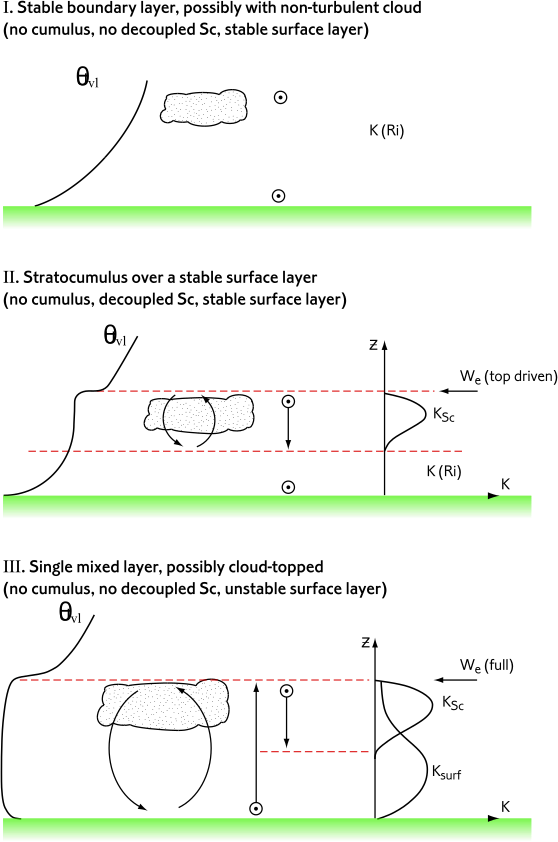
\includegraphics{wcrp_bltypes1}}
  \scalebox{0.46}{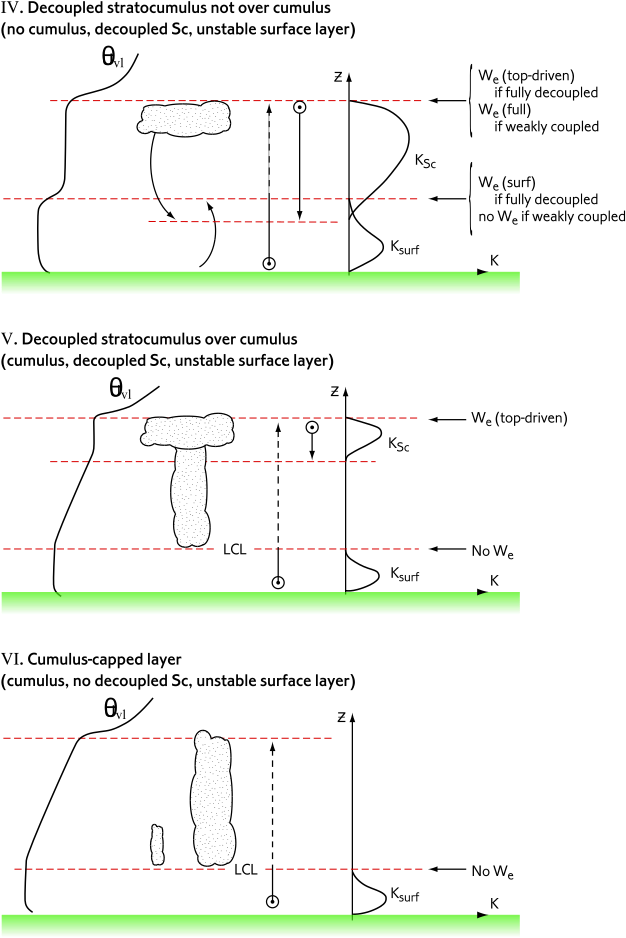
\includegraphics{wcrp_bltypes2}}
  \captionarb{Schematic representation of boundary layer types I to
    VI.  The top of the upward arrows indicate the height \zhpar while
    the top of their solid line portions indicate \zh.}
  \label{fig:bltypes}
\end{figure}

\subsection{The diagnostic parcel ascent and cumulus diagnosis}
\label{sec:adiapar}

{\bf Summary}: the depth of the non-local $K$-profiles for
surface-driven turbulence (with NTML grid-levels in the mixed layer
and top at height \zh, as required for (\ref{kmsurf})) is determined
from:
\begin{enumerate}
\item a diagnostic moist parcel ascent; top at grid-level NTPAR,
  height \zhpar$=z_{\ntpar+\frac{1}{2}}$.  Typically this is an
  adiabatic parcel but entraining options are available.
\item a diagnosis of cumulus-capped layers (if cumulus-capped then
  NTML and \zh are set to the LCL\footnote{unless the option to mix
    across the LCL is selected, see section~\ref{sec:lclmixing}}, if
  not then to the parcel top)
\end{enumerate}
Note that this process is only performed for unstable boundary layers
(defined by a positive surface buoyancy flux, \mbox{i.e.}, $\wbs>0$).

{\bf Step 1:} the method assumes that the height to which turbulent
mixing driven by surface processes can extend in unstable boundary
layers (and therefore the vertical extent of the $K$ profile for
surface-driven turbulence) can be determined solely from the
properties of the thermodynamic profiles.  In more detail, the first
step in calculating \zh is to lift a parcel, with properties from the
first grid-level ($k=k_s$) above the top of the surface layer, upwards
allowing for latent heat release.  The top of the surface layer is
taken to be at the lower of $z=0.1$\zh (this is then consistent with
the $K$-profiles, see section~\ref{sec:nlsurf}; \zh is taken from the
previous timestep) and the grid-level above which $\thetavl$ starts to
increase with height.  The ascent is stopped at the grid-level NTPAR
(height \zhpar$=z_{\ntpar+\frac{1}{2}}$) above which the parcel
becomes more negatively buoyant than a given threshold, $\theta_v'$.
Note that the parcel properties themselves are not perturbed in order
to preserve the height of the mixed-layer's lifting condensation level
(LCL).  The calculation of the parcel's buoyancy excess is described
in section~\ref{sec:parxs}.  Currently,
\begin{equation}
  \theta_v' = \mbox{max} \left[A_{plume}, 
           \, \mbox{min} \left[ B_{plume} \sigma_{Tv1}, 
           \, G_{max}\zhe \right] \right]
  \label{parcel_pert}
\end{equation}
where $A_{plume}=0.2$, $B_{plume}=3.26$, $G_{max}=10^{-3}$Km$^{-1}$,
$\sigma_{Tv1} = 1.93\, \wthvs/w_m$ and $w_m^3=u_*^3+0.25\,\zhe \wbs$.
Following \cite{holtslag93:_local_versus_nonloc_bound_layer},
$\theta_v'$ is related to the magnitude of the gradient adjustment,
$\gamma_{\thetal}$ (see section \ref{sec:gradadj}).  Thus,
$B_{plume}=A_{ga}$, although somewhat arbitrary limits have been
placed on the magnitude of $\theta_v'$ for numerical security (the
upper limit being consistent with that applied to $\gamma_{\thetal}$
in (\ref{gradadj}) ).  Within limits, then, $\theta_v'$ represents a
typical buoyancy excess of boundary layer plumes.

The pressure at the LCL, $P_{LCL}=P_{k_s}
(T_{LCL}/T_{k_s})^{(1/\kappa)}$, where $\kappa=R/c_p$.  The
temperature at the LCL, $T_{LCL}$, is calculated using approximations
in \cite{Bolton1980} as
\begin{equation*}
  T_{LCL} = 55 + \frac{2840}{3.5 \log(T_{k_s}) - log(e_{k_s}) - 4.805}
\end{equation*}
where the vapour pressure of air in grid-level $k_s$, $e_{k_s} =
q_{k_s} P_{k_s}/(100 \, \epsilon)$.  The full-level below that
containing the LCL is labelled NLCL and \zlcl$=z_{\nlcl+\frac{1}{2}}$.
If the parcel rises above the top of the LCL transition zone (defined
as 1.1\zlcl, its ascent can also be stopped at the grid-level at which
it has maximum buoyancy excess over the environment.  This is
identified as the grid-level above which
\begin{equation*}
  \frac{d\theta_v}{dz}|_{\rm env} > 
  \Gamma_{\rm inv}\, \frac{d\theta_v}{dz}|_{\rm par} 
\end{equation*}
where currently the tolerance for identifying inversions by this
method, $\Gamma_{\rm inv}=1.1$.  This use of the height of maximum
excess (if lower than that given by the straight buoyancy threshold,
$\theta_v'$) is typically of little consequence in stratocumulus
regions (which tend to be well-mixed beneath large inversions), but
can be necessary in order to identify the capping inversion in cumulus
cases (e.g.~in the trade wind regions).

{\bf Step 2:} having established \zhpar, a crucial additional test is
to determine whether this layer is well-mixed (\mbox{i.e.},
stratocumulus-capped) or cumulus-capped.  The parcel ascent can rise
to cloud-top in both cases but cumulus cloud layers are observed not
to be as well-mixed as stratocumulus layers.  Recall that application
of the $K$ profiles is expected to form or maintain well-mixed layers
and so their current formulation is inappropriate for cumulus cloud
layers.  Specifically, a logical flag (CUMULUS) is set to true if
\begin{equation*}
         \left| \frac{ \Delta_{\rm cld} q_t}{\Delta_{\rm cld} z} \right| > 
  C_t \, \left| \frac{ \Delta_{\rm sub} q_t}{\Delta_{\rm sub} z} \right|
\end{equation*}
where the cloud-layer gradient, $ \Delta_{\rm cld} $, is taken between
both NTPAR and NTPAR-1 (to allow for the possibility that a Sc layer
has just deepened by a grid-level) and NLCL and the sub-cloud layer
gradient, $\Delta_{\rm sub}$, between grid-levels NLCL and $k_s$.
Currently the threshold factor, $C_t = 1.1$.  If cumulus is diagnosed,
the top of the surface-based mixed layer (\zh) is set to \zlcl (rather
than to \zhpar, as illustrated in Fig.~\ref{fig:bltypes} for types V
and VI).  There is then an option to diagnose the thickness of the LCL
transition zone, see section~\ref{sec:lclmixing}.  Otherwise, the
boundary layer surface-driven mixing is capped at \zlcl so that mixing
into the cumulus cloud layer is only carried out by the model's
mass-flux convection scheme and not by the eddy viscosity based
boundary layer scheme.  Note that basing the CUMULUS diagnosis on
cloud and sub-cloud layer gradients limits the model only to being
able to resolve cumulus with cloud and sub-cloud layers at least 2
grid-levels (and optionally 400m) thick.  Otherwise the layer is
considered well-mixed to \zhpar with an option to include a
representation of fluxes into the capping inversion (see
section~\ref{sec:dzi}).

If the parcel ascent fails to find an inversion below 3km (or
BL\_LEVELS) but the LCL is below BL\_LEVELS, then the layer is assumed
to be cumulus-capped.  If the LCL is above BL\_LEVELS, then again
cumulus is diagnosed with NTML$=\mbox{min}[$NLCL, BL\_LEVELS$-1]$, in
the hope that the mass-flux convection scheme (in its moist or dry
mode) will transport the surface fluxes higher! Clearly this
restriction on the boundary layer scheme is not desirable and so a
value of BL\_LEVELS above the tropopause is recommended.

Note that if cumulus is not diagnosed then a further, subgrid
estimation of the height of the capping inversion is attempted for \zh
(as described in section~\ref{sec:sginv}).

\subsubsection{Calculation of parcel buoyancy excess}
\label{sec:parxs}

As described in appendix~\ref{app:buoyp}, virtual temperature, $T_v =
T(1 + c_v q_v - \ql - q_f)$, is used as the measure of buoyancy.  The
condensed water in the parcel at a grid-level $k$ ($\qlf^p$, the
superscript $^p$ indicating parcel properties) is estimated using a
Taylor expansion of $q_s$ about the environment at that grid-level
($q_s^p \approx {q_s}_k + \alpha_L (T^p-T_k) $).  Assuming that
$\qlf^p=q_t^p - q_s^p$ gives
\begin{equation}
  \qlf^p = \mbox{max}\left[ 0.0, \, a_L \left( q_t^p - {q_s}_k 
         - \alpha_L (\thetal^p - (g z_k/c_p)-T_k)\right) 
  \right]
  \label{qlpar}
\end{equation}
where the buoyancy parameters $a_L$ and $\alpha_L$ are defined in
appendix \ref{app:buoyp}.  Recall that the parcel has $q_t$ and
$\thetal$ taken from grid-level $k_s$ which are conserved during its
ascent.  Note that (\ref{qlpar}) will not give condensation until the
parcel becomes saturated.  In the environment the cloud scheme will
allow some condensation (and therefore warming and stabilisation of
the environment profile) to take place before the grid-level becomes
saturated in the mean.  To allow for this in the parcel (without
applying the cloud scheme), (\ref{qlpar}) is also calculated at each
grid-level but using the environment grid-box mean $q_t$ and $\thetal$
to give $\qlf^e$.  The difference in the environment's condensed water
as determined by the UM cloud scheme (\mbox{i.e.}, $\ql+q_f$) and by
(\ref{qlpar}) (\mbox{i.e.}, $\qlf^e$) is then added to $q^p_{lf}$.

Given $\qlf^p$, (\ref{thetal}) implies $T^p = \thetal^p - (g z_k/c_p)
+ (L \qlf^p/c_p)$ (using $L_s$ if $T_k$ is below the melting point)
and (\ref{qt}) implies $q_v^p = q_t^p - \qlf^p $ and thus $T_v^p$ can
be calculated.  Recall that the diagnosis of the parcel's maximum
buoyancy excess over the environment (described in
section~\ref{sec:adiapar}) required $\theta_v$.  This is approximated
as $\theta_v = T_v + (g z_k/c_p)$.

\subsection{Diagnosis of the vertical extent of the K-profiles}
\label{sec:decouple}

The diagnosis of mixed layers with turbulence driven from cloud-top
has been separated in to three stages.  These are:
\begin{enumerate}
\item diagnose the existence of a decoupled stratocumulus (DSC) layer
  with approximately uniform $\thetavl$ (label the top grid-level in
  the mixed-layer NTDSC and diagnose the subgrid height of its capping
  inversion, \zhsc, see section~\ref{sec:sginv})
\item diagnose an approximate depth of the DSC layer, $\zml$, in order
  to be able to calculate the representative turbulent velocity scales
  (see appendix \ref{app:vscales}).
\item calculate the depth of the $K$ profiles (see
  section~\ref{sec:nonlocal}) in both SML and DSC layers using
  constraints on the TKE budget of the layer.  This includes the
  diagnosis of recoupling of DSC layers and decoupling of SMLs
\end{enumerate}

{\bf Step 1}: the diagnosis of DSC layers depends on whether cumulus
convection has been diagnosed.  If a cumulus-capped layer under an
inversion within BL\_LEVELS has been diagnosed, grid-levels NTPAR and
NTPAR+1 are tested to see if they contain significant layer cloud
($C_F>$ SC\_CFTOL).  This threshold for identifying potentially
turbulently-mixed cloud layers is currently SC\_CFTOL$=0.1$.  If there
is significant cloud, NTDSC is set to NTPAR.

Alternatively, if a well-mixed surface-driven boundary layer was
diagnosed, then from grid-level NTML$+2$ upwards, a cloud-top
grid-level ($k_{ct}$) is sought such that ${C_F}_{k_{ct}}>$ SC\_CFTOL
and ${C_F}_{k_{ct}+1}<$ SC\_CFTOL.  If $\Delta_{k_{ct}} \thetavl /
\Delta_{k_{ct}} z < 10^{-3}$Km$^{-1}$ (\mbox{i.e.}, $\thetavl$ is
approximately well-mixed over at least two grid-levels), then NTDSC is
set to $k_{ct}$.  If grid-levels $k_{ct}$ and $k_{ct}-1$ are not
well-mixed, grid-levels $k_{ct}-1$ and $k_{ct}-2$ are tested using the
same criterion.  If they are not well-mixed either, the cloud-layer is
ignored for the purposes of turbulent mixing.  If grid-levels
$k_{ct}-1$ and $k_{ct}-2$ are identified as well-mixed a further test
is applied to determine whether the $\theta_v$ (rather than
$\thetavl$) gradient across grid-levels $k_{ct}$ and $k_{ct}-1$ is
greater than adiabatic (\mbox{i.e.}, whether grid-levels $k_{ct}$ and
$k_{ct}-1$ actually form part of an inversion --- note that by
ignoring the $\ql$ contribution to buoyancy, $\thetavl$ is not a good
variable to use to measure the strength of cloud-capping inversions).
To do this, the $\theta_v$ gradient between grid-levels $k_{ct}$ and
$k_{ct}-1$ is compared with that for a parcel lifted adiabatically
from grid-level $k_{ct}-1$, in exactly the same way as for the SML
parcel ascent (see section \ref{sec:parxs}).  If $d\theta_v/dz|_{\rm
  env} > \Gamma_{\rm inv} d\theta_v/dz|_{\rm par} $ between
grid-levels $k_{ct}$ and $k_{ct}-1$ then NTDSC is set to $k_{ct}-1$;
if not then NTDSC is set to $k_{ct}$ (recall that grid-levels
$k_{ct}-1$ and $k_{ct}-2$ have already been identified as well-mixed).

{\bf Step 2} is to diagnose an approximate depth of the DSC layer,
$\zml$.  The bottom grid-level of the mixed-layer (NBDSC) is diagnosed
as the lowest grid-level, descending from NTDSC, where
${\thetavl}_{\ntdsc} + \thetavl'$ is less than $\thetavl$ of the
environment.  The parcel perturbation is given by
\begin{equation}
  \thetavl' = - \, \frac{ \tau_{rc} \Delta_\radf }{z_{rc}}
  \label{dscd_pert}
\end{equation}
where $\Delta_\radf$ (Kms$^{-1}$) is the magnitude of the cloud-top
radiative divergence (see appendix~\ref{app:vscales}), $\tau_{rc}$ is
a timescale for the exposure of boundary layer eddies to the cloud-top
radiative cooling (taken to be 200s) and $z_{rc}$ is a depth-scale for
the radiatively cooled layer (taken to be 50m).  These values of
$\tau_{rc}$ and $z_{rc}$ are only estimates (and will in reality vary
from one cloud to another) but they are consistent with, for example,
the observations of \cite{nicholls1986}.  If the parcel failed to fall
(\mbox{i.e.}, NBDSC equals NTDSC) in a DSC layer {\em not} overlying
cumulus, then the layer is assumed not to be well-mixed.  At the top
of a cumulus layer, the DSC layer is given a minimum depth of
$\Delta_{\ntdsc+\frac{1}{2}} z$.  Otherwise, the layer depth, $\zml$,
is measured from the top of layer NTDSC to the base of layer NBDSC.

{\bf Step 3}: the step 2 calculation of $\zml$ is used to calculate
the representative velocity scales for the DSC layer but its
calculation is only crude.  Here, the vertical extent of the
$K$-profiles is determined more accurately by ensuring that the
magnitude of the integrated buoyancy consumption of TKE within the
mixed layer is less than or equal to a fraction, $D_t$, of the
buoyancy production, following \cite{turton1987}.

Following appendix~\ref{app:buoyp} the grid-box mean buoyancy flux can
be written as:
\begin{equation}
  \wb = g \left[ (1-C_F) \left(\beta_T \overline{w'\thetal'} + \beta_q \wqt \right) +
    C_F \left( \tilde{\beta_T} \overline{w'\thetal'} + \tilde{\beta_q} \wqt \right) 
  \right]
  \label{eq:wb_cont}
\end{equation}

As standard, the fluxes in (\ref{eq:wb_cont}) are then expanded using
the first-order closure in (\ref{scal_closure}) as:
\begin{eqnarray}
  \wthl_k &=&  -\khsurf \,\frac{\widetilde{\Delta_k \thetal}}{\Delta_k z}
               -\khtop \,\frac{\Delta_k \thetal}{\Delta_k z} \nonumber \\
  \wqt_k  &=&  -\left(\khsurf + \khtop \right) \,
               \,\frac{\Delta_k q_t}{\Delta_k z} 
  \label{eq:wx_std}
\end{eqnarray}
where $\widetilde{\Delta_k \thetal} = \Delta_k \thetal -
\gamma_{\thetal} \Delta_k z$ in order to include the non-local (or
gradient adjustment) term.  If the alternative flux-gradient option is
used, see section \ref{sec:rev_flux_grad}, then additional terms are
needed.

Large-eddy simulations have demonstrated that the crucial region in
determining when decoupling of stratocumulus will occur (\mbox{i.e.},
when the $K$ profiles no longer span the entire layer from cloud-top
to the surface) is in a thin layer of unsaturated air just below
cloud-base, where $\wb$ first becomes negative.  Thus, in the above
calculation, it is crucial both to have an accurate measure of
cloud-base height (which will have to be subgrid) and to include
successfully this thin unsaturated layer in the buoyancy consumption
integral.  Thus, the $\wb$ integration is performed over the cloud and
sub-cloud layers separately and the cloud-fraction is taken to be
uniform within the cloud layer (and zero below cloud-base).  The
height of cloud-base is given by (\ref{zc_calc}).

An iterative method is then used to find the vertical extent of mixing
(within certain bounds, as described below) such that the magnitude of
buoyancy consumption of TKE within the mixed layer equals a fraction,
$D_t$, of the buoyancy production, \mbox{i.e.},
\begin{equation}
  \sum_{z_{k-\frac{1}{2}} > z_i-\zml}^{z_{k-\frac{1}{2}} < z_i}
  \left|\left[ \wb|_{z_{k-\frac{1}{2}}}<0 \right]\right| \, \Delta_k z \, 
  \leq \, D_t \, 
  \sum_{z_{k-\frac{1}{2}} > z_i-\zml}^{z_{k-\frac{1}{2}} < z_i}
  \left[ \wb|_{z_{k-\frac{1}{2}}}>0 \right] \, \Delta_k z
  \label{deccrit}
\end{equation} 
Note that, for simplicity, the ${\cal E}_h$ factors are not included
in $\khsurf$ or $\khtop$ when calculating (\ref{eq:wx_std}) under the
assumption that they will be small.  This process is applied to all
unstable mixed layers.  For stratocumulus layers, observations and LES
suggest a value of $D_t=0.1$.  A separate value of $D_t$ can be used for 
the sub-cloud layer in cumulus capped boundary layers if this method is 
used to determine the LCL transition zone thickness, see 
section \ref{sec:lclmixing}.  For cloud-free mixed layers, $D_t=1$ is
used, purely to keep negative buoyancy fluxes down to a reasonably
realistic level (for example, if the parcel top diagnostic returned
too high a boundary layer depth).  

The first step is to test for whether a well-mixed layer is possible
(either decoupling what has so far been diagnosed as a well-mixed
layer or, if one exists, recoupling a decoupled stratocumulus layer),
\mbox{i.e.}, to test whether (\ref{deccrit}) is satisfied with both
$\khsurf$ and $\khtop$ extending from the surface to the cloud-top.
If recoupling is possible then the various flags identifying the DSC
layer are reset ({\em this includes setting the cumulus diagnosis to
  false}), any surface-driven entrainment originally applied at \zh is
added to the entrainment at \zhsc (after rescaling for the inversion
strength at \zhsc) and \zbase is set to 0.1\zh (for the reason
discussed above).  If decoupling is diagnosed, \zhsc is set to the
original \zh (inversion height), although the entrainment across this
inversion is not recalculated (and so keeps any surface-driven
component --- the COUPLED flag is therefore set to true, see
section~\ref{sec:entr}).

If a decoupled layer is diagnosed, then an iteration is performed to
find the highest \zh (so top of the $\khsurf$ profile) that still
satisfies (\ref{deccrit}), but with $\khtop=0$ in (\ref{eq:wx_std}).
The iteration proceeds with \zh stepping from its lowest permissible
height to its highest (currently 3 steps are used).  If at any stage
(\ref{deccrit}) is violated, then the step below (therefore containing
the height that would give equality in (\ref{deccrit})) is divided by
4 and 3 of those steps are taken downwards.  If (\ref{deccrit}) is met
the step above is again reduced by a factor of 4 and 3 steps taken
upwards.  A total of 3 sweeps are possible, each with a smaller step
so that \zh approaches the height that gives equality in
(\ref{deccrit}).  The accuracy with which this is achieved will be the
difference in the maximum and minimum permissible heights of \zh
divided by $2\times4\times4 = 32$, which will typically be less than
30m.  The top grid-level of the SML, NTML, is defined as the highest
grid-level such that $\khtop$ is non-zero at the half-level above.

The above process is then repeated to find the appropriate \zbase for
$\khtop$, \mbox{i.e.}, for the base of top-driven mixing.  Some
constraints are placed on \zbase, namely that it should never go below
$0.1$\zh (to avoid affecting the continuity of the $K$ profiles at the
top of the surface layer, see (\ref{ws_defn})). If cumulus convection
has been diagnosed then \zbase is not allowed to go below
$z_{\ntml+\frac{1}{2}}$ (unless the layer is diagnosed to recouple
completely).  Finally, \zbase must always be at or below
$z_{\ntdsc-1}$, so that mixing in decoupled layers is always resolved,
and at least $\Delta z_{rad}$ (the cloud-top radiative cooling depth
defined in section \ref{sec:wbint_inv}) below the t inversion.  The
base grid-level of the DSC layer, NBDSC, is defined (analogously to
NTDSC) as the lowest grid-level such that $\khtop$ is non-zero at the
half-level below.

A possible extension to this diagnosis would be to include the shear
contribution to the TKE budget in (\ref{deccrit}) and so allow
shear-driven mixing to help maintain well-mixed layers.

\subsubsection{Surface layer $\wb$ integration}

In the surface layer, below $z_i/10$, the $K$ profiles have a
different functional form from the rest of the mixed layer.  Rather
than include this additional complexity in the $\wb$ integration, the
surface layer is treated separately.  In place of the
finite-difference form of $\wb$, see (\ref{eq:wb_cont}) and
(\ref{eq:wx_std}) above, $\wb$ is assumed to be linear between $\wbs$
at the surface and zero at a level which must be estimated.  The
surface layer integration is then from the surface up to $z_{{\rm
    K_{SURF}}}$, where $\theta$-level K\_SURF is the first above
$z_i/10$.  The level where $\wb$ is zero is found by linear
interpolation across the grid-levels where the diagnosed cloud-free
buoyancy flux would become negative.  This is where $\beta_T
\widetilde{\Delta_k \thetal} + \beta_q \Delta_k q_t$ becomes positive
and so where the cloud-free part of $\wb$ (\mbox{i.e.}, that part
below cloud-base which is important for decoupling) becomes negative.


\subsubsection{Integration of $\wb$ close to the inversion}
\label{sec:wbint_inv}

Because of the large gradients often seen in fluxes close to the
inversion (in particular, in the LW radiative flux), simple finite
difference flux calculations, (\ref{eq:wx_std}), can be significantly
inaccurate in this region.  An example is shown in
Fig.~\ref{fig:inv_integ}.  Calculating $\wthl_{\ntml+\frac{1}{2}}$
from (\ref{eq:wx_std}) gives a negative value, largely because
$\Delta_{\ntml+1} \thetal$ is positive and so the local flux is large
and negative.  In reality, $\wthl$ becomes positive only a short
distance below cloud-top such that the integral here will tend also to
be positive.

The solution adopted is to integrate $\wb$ analytically across the
region just below the inversion, labelled $\Delta z_{rad}$ in
Fig,~\ref{fig:inv_integ}.  Since $\Delta_{\ntml} \thetal$ can also be
significantly positive (when the grid-level inversion is rising or
falling, for example), the base of this region is taken to be the
lower of the first $\theta$-level below $z_h-100$ m (a physically
reasonable depth over which cloud-top radiative cooling might be
expected to occur) and $z_{\ntml-1}$.
\begin{figure}[tb]
  \begin{center}
    \scalebox{1}{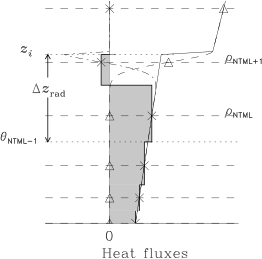
\includegraphics{ideal_invinteg}}
    \caption{Subgrid (lines) and model (symbols) fluxes of $\thetal$:
      turbulent flux (dash-dotted, crosses), radiative flux (dashed,
      triangles) and total flux (solid).  The shaded area illustrates
      the integrated turbulent flux that would be obtained were
      (\protect\mbox{\protect\ref{eq:wx_std}}) used.}
    \label{fig:inv_integ}
  \end{center}
\end{figure}
Then,
\begin{eqnarray}
  \int_{z_h-\Delta z_{rad}}^{z_h} \, \wthl \, dz  & = & 
  \int_{z_h-\Delta z_{rad}}^{z_h} \, F_{\thetal}^{Tot} -
  F_{\thetal}^{NT}\, dz
  \nonumber \\
  & = &  I^{Tot} - I^{rad} - I^{ppn}
  \label{wthl_int}
\end{eqnarray}
For the radiative flux, it could be assumed that the subgrid flux
distribution is exponentially dependent on the grid-level LWP, for
example.  This would give:
\begin{equation}
  I^{rad} = \frac{\Delta z_{rad}}
  {\ln(F^{rad}|_{z_h}/F^{rad}|_{z_h-\Delta  z_{rad}} ) }
   \lb F^{rad}|_{z_h}-F^{rad}|_{z_h-\Delta  z_{rad}} \rb
  \label{irad}
\end{equation}
However, off-line tests indicated this could give a strong and
spurious sensitivity to $F^{rad}|_{z_h-\Delta z_{rad}}$.  Furthermore,
for most realistic scenarios, the logarithmic factor in (\ref{irad})
tends to be close to 3.  Consequently, we approximate $I^{rad} =
\Delta z_{rad} ( F^{rad}|_{z_h}-F^{rad}|_{z_h-\Delta z_{rad}} ) /3 $.
In addition, $F^{rad}|_{z_h}-F^{rad}|_{z_h-\Delta z_{rad}} $ is
approximated as $\Delta \radf$, the radiative flux change across
cloud-top used in the calculation of $\vtopo$ (\ref{ctraddiv}).  The
precipitation flux is assumed to vary linearly across this region, as
does the total flux, and so its contribution to $I^{Tot}$ cancels with
$I^{ppn}$ in (\ref{wthl_int}).  Finally, for simplicity, the total
flux is taken to be constant and equal to the inversion value, such
that $I^{Tot} = \Delta z_{rad} F^{Tot}|_{z_h}$.  With these
approximations, (\ref{wthl_int}) becomes
\begin{eqnarray*}
  \int_{z_h-\Delta z_{rad}}^{z_h} \, \wthl \, dz  & = & 
  \Delta  z_{rad} \lb -w_e \Delta \thetal + \Delta \radf \rb 
  - \Delta z_{rad} \Delta \radf / 3 \\
  & = & \Delta  z_{rad} \lb -w_e \Delta \thetal + \frac{2}{3} \Delta \radf \rb 
\end{eqnarray*}
For the integral of $\wqt$ across this cloud-top region, $\wqt$ is
also taken to be constant so that:
\begin{equation}
  \int_{z_h-\Delta z_{rad}}^{z_h} \, \wqt \, dz = 
  - \Delta  z_{rad} w_e \Delta q_t
\end{equation}
The integrated buoyancy flux is then found from (\ref{eq:wb_cont})
using the mixed layer cloud fraction and buoyancy coefficients
evaluated at the grid-level above $ z_h -\Delta z_{rad} $.

\subsection{Diagnosis of inversion thickness}
\label{sec:dzi}

Terminating the diagnostic parcel ascent at its level of neutral
buoyancy ignores any overshooting through the parcel's own inertia as
it enters the inversion region.  This overshooting region effectively
defines the depth of the inversion over which the negative entrainment
heat fluxes are seen.  Typically this will be small relative to the
model vertical grid but at higher vertical resolution or when a
strongly surface-heated boundary layer is capped by weak stability
inversions could be resolved.  Following \cite{beare2008}, a simple
energetic argument gives a realistic prediction of the top of the
inversion, $z_{top}$, in LES from
\begin{equation}
  6.3 \, w_m^2  =  \int_{z_{nb}}^{z_{top}} \, b \, dz
  \label{dz_param}
\end{equation}
where $z_{nb}$ is the level of neutral buoyancy (found by linear
interpolation between grid-levels), $w_m$ is the boundary layer
velocity scale defined in section \ref{sec:nlsurf} and $b$ is the
parcel buoyancy.  Note that the constant in (\ref{dz_param}) is the
same as in \cite{beare2008} because $6.3 = 2.5 * 4^{2/3}$ and $w_m^3$
differs by a factor of 4.  The buoyancy integration in
(\ref{dz_param}), that is itself dependent on $z_{top}$, is performed
working upwards from \zhpar assuming piece-wise linear variation of
$b$ between grid-levels.  Note that the standard definition of the
boundary layer top in the UM is the height of the first flux level
below the level of neutral buoyancy, so
\zhpar$=z_{\ntpar+\frac{1}{2}}$.  The inversion thickness is then
defined as
\begin{equation}
  \Delta z_i  =  z_{top} -\zhpare
  \label{dz_definition}
\end{equation}

\subsection{Diagnosis of the LCL transition zone thickness}
\label{sec:lclmixing}

As described in section~\ref{sec:adiapar}, when cumulus convection has
been diagnosed surface-driven mixing was originally capped at \zlcl so
that mixing into the cumulus cloud layer was only carried out by the
model's mass-flux convection scheme.  This was seen to lead to errors
in the mean profiles across the LCL, with superadiabats being the most
extreme manifestation.  Using the boundary layer parametrization to
couple cloud and sub-cloud layers would have the numerical advantage
of being implicit.  There is also observational and LES evidence that
appropriately-scaled buoyancy fluxes up to the LCL are
indistinguishable from those in cloud-free convective boundary layers
and so the non-local surface-driven mixed layer K-profiles remain
accurate up to this level.  To diagnose the depth to which these
profiles should penetrate above the LCL, the algorithm given in
section~\ref{sec:decouple} to diagnose the extent of the K-profiles in
decoupled boundary layers can be used (using the switch kprof\_cu).
This ensures that the magnitude of the integrated buoyancy consumption
of TKE within the mixed layer is less than or equal to a fraction, $D_t$,
of the buoyancy production.  In cumulus layers, cloudy thermals will
generate positive buoyancy fluxes (and are handled by the convection
scheme) but it is assumed that there will also be cloud-free thermals
within the grid box that may penetrate above the grid-box mean LCL
(but are too dry to reach their own LCL).  Thus their buoyancy flux is
given by (\ref{eq:wb_cont}) with $C_F=0$.  Restricting the negative
integral of this buoyancy flux then gives a new definition for \zh
that is then used in the calculation of the surface-driven K-profiles
in section~\ref{sec:nlsurf} --- the larger the value of $D_t$, the 
higher \zh will be.  Typically $D_t=0.1$ for decoupled stratocumulus 
layers while idealised clear-sky convective boundary layers (where 
the magnitude of the entrainment buoyancy flux is a fraction, $A_1$, 
of the surface flux) would have $D_t = A_1^2 \sim 0.05$.  For GA7 $D_t$ 
has been set to 0.05 for this cumulus transition zone calculation.  
Because the Gregory-Rowntree convection scheme triggers from the LCL, that 
is used as a minimum constraint on the boundary layer mixing depth (so that 
the massflux and turbulence schemes remain coupled).  With other convection
schemes this may not be appropriate and so this minimum constraint can be 
relaxed, which is achieved by setting it to half the height of the LCL (the 
factor of a half is arbitrary, with no sensitivity to this choice given that 
the diagnosis parcel reached the LCL, but ensures the iteration starts well 
below the LCL).

%------------------------------------------------------------------------
% LOCAL SCHEME
%------------------------------------------------------------------------
\section{The local scheme}
\label{sec:local}

A first order `mixing length' closure is used:
\begin{eqnarray}
  K_m &=& {\cal L}_m^2 \, (S+S_d) \, f_m(Ri) \label{kmlocal}\\
  K_h &=& {\cal L}_h \, {\cal L}_m \, 
          (S+S_d) \, f_h(Ri) \label{khlocal}
\end{eqnarray}
where ${\cal L}_m$ and ${\cal L}_h$ are the neutral mixing lengths and
$S$ is the resolved vertical shear of the horizontal wind components,
$S = \left| \partial {\bf u}/\partial z \right|$.  A representation of
the wind shear, $S_d$, generated by drainage flows in complex terrain
can also be included, as described below.  Near the surface simple
finite difference calculations for the vertical gradients can become
inaccurate because of the quasi-logarithmic profiles of variables
\cite[]{Ayra1991}.  Currently this is ignored above grid-level 2 and
the neutral mixing lengths are given by
\begin{eqnarray*}
  {\cal L}_m &=& \frac{k(z+z_{0m})}{1+k(z+z_{0m})/\lambda_m} \\
  {\cal L}_h &=& \frac{k(z+z_{0m})}{1+k(z+z_{0m})/\lambda_h} 
\end{eqnarray*}
where $z_{0m}$ includes the orographic component.  For the lowest
interior grid-level ($k=1$) they are calculated, incorporating this
log profile correction, as
\begin{equation*}
  \tilde{{\cal L}}_{X,k-1/2} = \frac{k \Delta_{k-1/2} z}{ 
    ln\left( \frac{z_k + z_{0m}}{z_{k-1} + z_{0m}} \right) 
    + \frac{k \Delta_{k-1/2} z}{\lambda_X} }
\end{equation*}
If near-surface resolution is increased this logarithmic correction
should be considered over more levels.

The asymptotic mixing lengths are given by 
\begin{eqnarray}
  \lambda_m &=&\mbox{max}\left[\lambda_0,\, 0.15 \zloce, 2 h_B \right] \nonumber\\
  \lambda_h &=&\mbox{max}\left[\lambda_0,\, 0.15 \zloce \right]
  \label{asymp_ml}
\end{eqnarray}
where $\lambda_0$ is a minimum mixing length read in from the namelist 
and \zloc is defined below.  The orographic blending height, $h_B$ (only 
used within the boundary layer, as defined below), is given by
\begin{equation*}
  h_B = {\rm max}\left[z_1+(z_{0m})_{\mbox{veg}}, 2^{1/2} \sigma_h \right]
\end{equation*}
where $\sigma_h$ is the standard deviation of the height of the
subgrid orography and $(z_{0m})_{\mbox{veg}}$ is the vegetative part
of the roughness length.  The constants in (\ref{asymp_ml}) can be
considered `tuned' (see, in particular, the operational modifications
described in appendix~\ref{app:opmods}).

The Richardson number, $Ri$, that is used as a local measure of
stability is given by
\begin{equation}
  Ri = \frac{\Delta B / \Delta z}{(S+S_d)^2}
  \label{ridefn}
\end{equation}

The measure of buoyancy used in $Ri$ is 
\begin{equation}
  \Delta B = g\left(   \overline{\beta_T} \Delta \thetal
           + \overline{\beta_q} \Delta q_t    \right)
  \label{Bdefn}
\end{equation}
where $\overline{\beta_T}$ and $\overline{\beta_q}$ are the grid-box
mean (\mbox{i.e.}, cloud weighted) buoyancy coefficients, that can be 
defined in two different ways, see appendix~\ref{app:buoyp} and 
section~\ref{sec:fd_ri}.  Note that (\ref{Bdefn}) reduces
to a virtual temperature approximation of buoyancy in cloud-free air
and that neutral buoyancy (in cloudy as well as cloud-free air) is
implied by vertically uniform $\thetal$ and $q_t$.  This is then
entirely consistent with the assumption that $\thetal$ and $q_t$ are
conserved variables within the boundary layer scheme.

As described in \cite{lock2012}, the wind shear generated by drainage
flows in complex terrain is thought to lead to additional vertical
mixing.  This wind shear can be approximated as
\begin{equation*}
  S_d = \frac{\Delta B }{ \Delta z} \, \alpha_d \, t_d \, {\cal Z}_d
\end{equation*}
The representative slope of the local terrain, $\alpha_d$, is given by
\begin{equation*}
  \alpha_d^2 = \frac{1.0}{ 25.0 + (l_h/\sigma_h)^2}
\end{equation*}
with $l_h$ a specified horizontal scale for the terrain, currently
taken to be 1500 m (empirically derived for Scottish orography in the
UKV), and $\sigma_h$ the standard deviation of the full subgrid
orographic height.  $\sigma_h$ should also be taken as the average
over the surrounding area of each grid box (typically 6 to 8 grid
lengths), in order to be representative of the local area over which
such flows will be underresolved.  The above formula is used so that
$\alpha_d \sim \sigma_h/l_h $ for small $\sigma_h$ but only tends to
0.2 for large values.  To limit the vertical extent of $S_d$ to be
below approximately $z=\sigma_h$, a height-dependent factor is
included, ${\cal Z}_d = 0.5( 1 - {\rm tanh}\left[ 4 ((z/\sigma_h)-1)
\right])$.  The timescale, $t_d$, takes a fixed value of 30 minutes,
for simplicity.

Initially, the lowest half-level at which $Ri>Ri_{crit}$ is taken to
be a measure of the boundary layer top (\zloc) and the full-level
below is designated NTLOC.  In general $Ri_{crit}=1$ but a value of
0.25 is recommended for use with the 'SHARPEST' stability functions,
see below.  If the boundary layer was diagnosed as cumulus-capped by
the non-local scheme (see section~\ref{sec:types}) then \zloc is
lowered to \zlcl (and $K_h$ and $K_m$ are set to zero from the base of
grid-level NLCL upwards) so that transports into and within the
cumulus cloud layer can be performed solely by the mass-flux
convection scheme.  Depending on the switch local\_fa, above NTLOC 
turbulently-mixed layers (where $Ri<Ri_{crit}$) are identified 
and within each layer \zloc in (\ref{asymp_ml}) is set to the layer 
thickness.  Outside of these turbulent layers the mixing lengths 
are set to $\lambda_0$.

For $Ri < 0$, the standard UM stability functions are given by 
\begin{eqnarray}
  f_m & =& 1 - \frac{g_0 \,Ri}
          {1+D_m(\tilde{{\cal L}}_m/\tilde{{\cal L}}_h)|Ri|^{1/2} } \nonumber\\ 
  f_h & =& \frac{1}{Pr_N}\left(1 - \frac{g_0 \,Ri}
          {1+D_h(\tilde{{\cal L}}_m/\tilde{{\cal L}}_h)|Ri|^{1/2} }\right) 
\end{eqnarray}
\label{unstable_stab}
with $g_0=10$, $D_m=g_0/4$ and $D_h=g_0/25$. If the stability
dependent Prandtl number option is chosen (see below) the neutral
Prandtl number, $Pr_N$, is set to $0.7$; otherwise
$Pr_N=1$. Alternatives are those from the Met Office large-eddy model
(LEM), \cite{brown1999}:
\begin{eqnarray}
  f_m & =& (1 - c_{LEM} Ri)^{1/2} \nonumber\\
  f_h & =& \frac{1}{Pr_N}\left(1 - b_{LEM} Ri\right)^{1/2}
\end{eqnarray}
\label{unstable_stab_lem}
where $Pr_N = 0.7$, and the constants $b_{LEM}$ and $c_{LEM}$ can take
the values 40 and 16 respectively in the ``standard'' LEM model or
both be 1.43 in the ``conventional'' model.

For stable conditions ($Ri > 0$), several forms for the stability 
functions are available.  The `long-tailed' functions are
\begin{equation*}
  f_{\rm stable} = \frac{1}{1+g_0 Ri}
\end{equation*}
Alternative functions, which decrease as $1/Ri^2$ with increasing
stability are, from \cite{louis1979}:
\begin{equation*}
  f_{\rm stable} = \frac{1}{(1+ 5 Ri)^2}
\end{equation*}
and the family of ``sharp'' functions can be written in terms of a transitional 
Richardson number, $Ri_{t}$, as:
\begin{equation*}
  f_{\rm stable} = 
\begin{cases}
  (1 - 5Ri)^2 & {\rm for}\ 0<Ri<Ri_{t} \\
  (A_{Ri} + B_{Ri} Ri)^{-2} & {\rm for}\ Ri>Ri_{t}
\end{cases}
\end{equation*}
where 
\begin{eqnarray}
A_{Ri} & = & \left(1-g_0 Ri_{t}\right)/\left(1- g_0 Ri_{t}/2\right)^2  \nonumber\\
B_{Ri} & = & (g_0/2) /\left(1 - g_0 Ri_{t}/2\right)^2
\end{eqnarray}
For the `SHARPEST' function of \cite{derbyshire1997}, $Ri_{t}=0.1$, while 
larger values give even sharper reduction of turbulence with increasing $Ri$.
An additional option, used operationally in some configurations (originally 
in the Mesoscale Model, hence called 'MES tails'), is to blend linearly 
from Louis functions at the surface to SHARPEST by 200m.  

A stability dependent Prandtl number ($Pr=f_m/f_h$) is generally used 
following \cite{MailhotLock2004} with:
\begin{equation*}
  Pr=\min \left( Pr_{\rm max}, \, Pr_N(1+2Ri) \, \right).
\end{equation*}
The maximum permitted Prandtl number, $Pr_{\rm max}$, is currently set
to $5$ for model stability reasons. The stability functions for $Ri>0$ are 
then given by:
\begin{eqnarray*}
  f_m & =& \frac{Pr}{Pr_N} \, f_{\rm stable} \\
  f_h & =& \frac{1}{Pr_N}  \, f_{\rm stable} 
\end{eqnarray*}
Note that writing the functions in this way ensures that $f_m=1$ under 
neutral conditions and the effect of the variation in $Pr$ is for $f_m$ 
to decrease slower with increasing $Ri$ than $f_{\rm stable}$, which can 
be explained through increasing gravity-wave activity.

Finally, the LEM stable functions are also available which cut off all 
turbulence beyond a critical Richardson number, $Ri_c=0.25$:
\begin{eqnarray*}
  f_m & =& \left( 1 - \frac{Ri}{Ri_c} \right)^4 \\
  f_h & =& \frac{1}{Pr_N} \left( 1 - \frac{Ri}{Ri_c} \right)^4 (1 - g_{LEM} Ri)
\end{eqnarray*}
\label{stable_stab_lem}
with $g_{LEM}=1.2$.

\subsection{Finite difference calculations}
\label{sec:fd_ri}

The Charney-Phillips vertical grid staggering used in the UM stores
the horizontal wind components ($u$, $v$) on grid-levels,
$\rho$-levels, that are staggered relative to scalar variables (such
as $\thetal$ and $q_t$) and vertical velocity, $w$.  While much of the
boundary layer scheme is grid-independent, this has serious
implications for the calculation of $Ri$.  There are two obvious
possibilities, to calculate $Ri$ (and thence $K(Ri)$) on either
$\theta$-levels or $\rho$-levels and then interpolate either $K_h$ or
$K_m$ to be able to calculate the required fluxes.  To do the former
requires averaging the buoyancy gradient in the numerator (and is
referred to by \cite{cullen1994} as the `$\theta$-bar' method), the
latter the wind shear in the denominator (referred to as the
`$\rho$-bar' method).  Single-column model and other tests
demonstrated that the `$\rho$-bar' method could readily generate
instabilities just above the top of the boundary layer because
averaging the wind shear into this stable air tended to reduce $Ri$
and so promote mixing.  Fortunately, the `$\theta$-bar' method tended
to increase $Ri$ above inversions and so damp mixing.  Thus, $Ri$ is
calculated on $\theta$-levels as
\begin{equation*}
  Ri_k = \frac{DBDZ_k}
         {(\Delta_{k+\frac{1}{2}} {\bf u}/\Delta_{k+\frac{1}{2}} z)^2}
\end{equation*}
The buoyancy gradient on $\theta$-level $k$ can be calculated in two different ways, 
depending on the switch {\rm i\_interp\_local}.  The long-standing method is given by
\begin{equation*}
  DBDZ_k = g\left( \overline{\beta_T}_{k} (D\thetal DZ)_k
         + \overline{\beta_q}_{k} (Dq_t DZ)_k    \right)
\end{equation*}
where $\overline{\beta_T}$ and $\overline{\beta_q}$ are the grid-box
mean (\mbox{i.e.}, cloud-fraction weighted) buoyancy coefficients,
defined in appendix~\ref{app:buoyp}.  Note that because this is
defined on $\theta$-levels, no vertical interpolation of cloud
variables (fractional area and water contents), to which the buoyancy
coefficients are very sensitive, is required.  The volume-weighted
gradients of $\thetal$ and $q_t$ are calculated as
\begin{equation}
  (D\chi DZ)_k =\left( (z_{k}-z_{k-\frac{1}{2}}) \, \frac{\Delta_{k+1} \chi}{\Delta_{k+1} z} +
    (z_{k+\frac{1}{2}}-z_{k}) \, \frac{\Delta_{k} \chi}{\Delta_{k} z}
  \right) / \Delta_{k+\frac{1}{2}} z
\label{gradient_interp}
\end{equation}
as long as $\chi_{k-1}$ is defined on an atmospheric model level. To calculate 
$DBDZ_1$, between the surface and the lowest $\theta$-level, either the buoyancy gradient
from level 1 to 2 can be extrapolated, \mbox{i.e.},
\begin{equation*}
  (D\chi DZ)_1 = \frac{\Delta_{2} \chi}{\Delta_{2} z} 
\end{equation*}
or surface properties can be used.  Over sea, the sea-surface temperature 
and $q_{sat}$ can be used.  Over a heterogeneous (tiled) land surface the 
appropriate moisture variable varies between tiles.  For the orographic form drag 
(\ref{section_2}), an average $Ri_{SL}$ of the surface layer is calculated but, as 
discussed above, subsequent vertical averaging of $Ri$ would potentially be 
numerically unstable.  In principle, the tile-average of $(Dq_t DZ)_1$ could 
be calculated but for now, over land, the grid-box average surface temperature is 
used to calculate $(D\thetal DZ)_1$ and $(Dq_t DZ)_1$ is extrapolated from 
above (\mbox{i.e.}, $(Dq_t DZ)_1 = (Dq_t DZ)_2)$).

As noted above, a feature of the previous option is that applying the cloudy 
buoyancy coefficients at a cloud top level, $k$ say, to strong gradients 
interpolated between $k-1$ and $k+1$, can yield an unstable $DBDZ_k$ despite 
strong static stability, especially when the upper level is very dry.  This can be 
related to cloud-top entrainment instability but this process is intended to be 
represented within the non-local scheme.  Hence, the alternative method is to 
calculate the buoyancy gradient directly on $\rho$-levels and then interpolate this 
vertically to give $DBDZ_k$, using (\ref{gradient_interp}).  This then 
requires a cloud fraction on $\rho$-levels.  The difficulty comes where there is 
a change in cloud fraction between levels.  For this ``edge'' fraction, $f_{edge}$ 
(the fraction of the grid-box that is cloudy in one level but not in the other), the 
change in supersaturation ($ s = q_t-q_{sat}$) between 
levels is used to estimate the vertical fraction likely to contain cloud, $f_{lev}$.  
For example, where $C_F$ decreases with height, $f_{lev}={q_c}_{k-1}/(s_{k-1}-s_{k})$, 
where $q_c$ is the total condensate, and $f_{lev}$ also constrained to be less 
than unity.  The total cloud volume fraction 
is then given by $f_{tot} = {\rm min}[{C_F}_{k-1},{C_F}_k] + f_{edge}f_{lev}$ and this 
is used to weight the saturated contribution to the buoyancy parameters on 
$rho$-levels, \mbox{e.g.},
$\overline{\beta_T}_{k-1/2} = f_{tot} \tilde{\beta_T}_{k-1/2} + (1-f_{tot}){\beta_T}_{k-1/2})$,
where the saturated and unsaturated buoyancy parameters are also intepolated to 
$\rho$-levels using (\ref{gradient_interp}).

Having calculated $Ri$ on $\theta$-levels, ${K_m}_{k}$ and ${K_h}_{k}$
are calculated, still on $\theta$-levels, as in (\ref{kmlocal}) and
(\ref{khlocal}).  Finally, $K_h$ must be interpolated to
$\rho$-levels:
\begin{equation*} 
  {K_h}_{k+\frac{1}{2}} = \left(
    (z_{k+\frac{1}{2}}-z_{k}) {K_h}_{k+1} +
    (z_{k+1}-z_{k+\frac{1}{2}}) {K_h}_{k} \right) / \Delta_{k} z
\end{equation*}
Note that in the code the convention is for fluxes to be held on the
half-level below the variable itself.  Consequently, RHOKM(K), and
therefore RI(K), are held on the `half-level' below $\rho$-level K,
which is $\theta$-level K-1.

In addition to the above, the log profile correction applied to ${\cal
  L}_h$ (to give $\tilde{{\cal L}}_h$) must be applied {\em after}
interpolation of $K_h$ to level $k+\frac{1}{2}$ in order that the
correct cancellation with the finite difference scalar gradient in the
flux calculation can occur.  In the unstable stability functions
(\ref{unstable_stab}), however, $\tilde{{\cal L}}_h$ must be
calculated on $\theta$-levels (\mbox{i.e.}, the same as $\tilde{{\cal
    L}}_m$ and $Ri$) in order to maintain the same stability
dependence.

\subsection{Shear-driven mixing and interaction between the local and
  non-local schemes}
\label{sec:shear}
The general approach is to take $K_{\chi}$ in (\ref{scal_closure}) and
(\ref{uv_closure}) as
\begin{equation}
  K_{\chi} = \mbox{max} \left[ (K_{\chi}^{\rm surf}+K_{\chi}^{\rm Sc}), 
                              K_{\chi}(Ri) \right]
  \label{klnl}
\end{equation}
As noted in section~\ref{sec:closure}, this implies that mixing in
stable boundary layers is determined exclusively by the local scheme,
$K_{\chi}(Ri)$.  Continuing to calculate $K_{\chi}(Ri)$ in unstable
boundary layers and using (\ref{klnl}) is seen as the simplest way of
achieving a relatively smooth transition between stable and unstable
boundary layers.

At the top of unstable mixed layers, great care is taken to ensure the
parametrized entrainment mixing is implemented faithfully, see
section~\ref{sec:entr}).  Consequently, if a subgrid inversion has
been diagnosed capping a mixed layer (see section~\ref{sec:sginv}),
then $K_{\chi}(Ri)$ is set to zero at the interfaces either side of
the inversion grid-level.  There are also options (using the switch
Keep\_Ri\_FA) to set $K_{\chi}(Ri)$ to zero entirely above unstable
boundary layers or across the LCL in cumulus-capped layers.

However, the mixed-layer depths were only diagnosed from thermodynamic
constraints.  In near neutral boundary layers, shear generation of
turbulence might be expected to allow mixing to extend into regions of
weak static stability (and potentially to inhibit the formation of
cumulus).  Currently, therefore, if NTLOC$>$NTML+1 (in layers that are
not cumulus-capped) $K_{\chi}(Ri)$ is left unconstrained by the SML
part of the non-local scheme (and so not set to zero from the SML
inversion upwards) and similarly if NTLOC$>$NTDSC+1.  It is realised
that this does not cover the case of shear-driven mixing into cloud
layers that have been diagnosed as cumulus-capped (which would be
poorly represented by the current convection scheme).  Several methods
have been introduced that attempt to alleviate this problem, giving
rise to the diagnosis of a ``shear-dominated boundary layer'' type
(type VII), discussed in section~\ref{sec:types}.  The first (the
``shear-dominated boundary layer fix'') simply sets the CUMULUS flag
to false if NTLOC $>$ NTPAR.  This then ensures that the
locally-determined $K$ are not set to zero above the LCL.  Several
more rigorous options are available that incorporate a ``dynamic
criteria'' in the diagnosis of boundary layer type.  The first of
these prohibits the diagnosis of cumulus boundary layers when the bulk
measure of stability, $-z_i/L$, is small (currently less than 1.6).  
Here $z_i$ is taken as the top of the diagnosis parcel ascent (or at
most 3km) and $L$ is the surface Obukhov length.  This test also resets 
the depth of the surface-based mixed layer to level 1 since the top of 
the parcel ascent may not be suitable (having previously 
been diagnosed as cumulus cloud top).  The second method
effectively increases the importance of the Richardson number
diagnosis and has been developed from analysis of cold-air outbreaks
\cite[]{bodas-salcedo2012}.  Because of the strong surface buoyancy
generation of turbulence in these regimes, a calculation of $Ri$ is
made that allows for the gradient adjustment by the non-local scheme,
\mbox{i.e.}, using $\widetilde{\Delta_k \thetal}$ (see
(\ref{eq:wx_std})).  The height, \zloc, where $Ri>Ri_{crit}=0.25$ is
found.  It is then hypothesised that this level of turbulent
instability (that incorporates the effects of shear) only needs extend
some fractional distance into the cloud layer to disrupt the formation
of cumulus elements.  Thus, if $\zloce > \zlcle + f_{\rm sh}
\left(\zhpare-\zlcle\right) $, where $f_{\rm sh}$ is a tunable
parameter ($0<f_{\rm sh}<1$), then the convection scheme triggering is
suppressed (the CUMULUS flag is set to false) and the top of the
non-local surface-based mixing coefficient is reset to \zhpar (as it
would have been before convection was diagnosed from the parcel
ascent).

A diagnostic is calculated, ZHT $=\mbox{max}[\zhe, \zhsce, \zloce]$,
that gives a measure of the maximum height of turbulent mixing (STASH
3,304).  Recall, \zloc is the boundary layer depth diagnosed by $Ri >
Ri_{crit}$, \zhsc is the top of any stratocumulus layer and \zh is the
top of surface-based mixed layer, found by adiabatic parcel ascent but
reset to the LCL in cumulus capped layers.  Another diagnostic is
available, the ``boundary layer depth'' (STASH 25), that is set to
$=\mbox{max}[\zhe, \zloce]$ and so represents the depth of the stable
boundary layer or ``surface'' mixed layer.  Also available are three
diagnostics that represent the calculated value of each of the
individual terms in STASH 3,304: 3,356 is set to \zh; 3,357 is \zhsc
and 3,358 is \zloc.

%------------------------------------------------------------------------
% NON-LOCAL SCHEME
%------------------------------------------------------------------------
\section{The non-local scheme}
\label{sec:nonlocal}

This method of calculating $K$ values for unstable conditions is
non-local in the sense that, at a given height within the boundary
layer, $K$ is determined not by any local properties of the mean
profiles at that height but solely by the magnitude of the turbulence
forcing applied to the layer (as measured by the representative
velocity scales described in appendix~\ref{app:vscales}) and the
height within the layer.  The non-local scheme is therefore
particularly robust but care must be taken where the profiles are
applied.  The calculation of the vertical position and extent of the
$K$ profiles is described in section~\ref{sec:types}.

\subsection{Surface-driven turbulence}
\label{sec:nlsurf}

For turbulence sources at the surface (namely surface drag with
velocity scale $u_*$, and positive surface buoyancy fluxes with
velocity scale $w_*$) in a layer with top at $z=$\zh, base at $z=0$ we
set
\begin{equation}
  \kmsurf = k \ \zhe \ w_m \ \frac{z}{\zhe}
            \left( 1 - {\cal E}_m^{\rm surf} \frac{z}{\zhe} \right)^2
  \label{kmsurf}
\end{equation}
where $w_m^3 = u_*^3 + w_s^3$, $u_*$ is the friction velocity
(including the orographic roughness component) and $w_s$ is defined
below.  For the 9C version of the scheme, \zh is the
diagnosed subgrid inversion height (see section~\ref{sec:sginv}) for
both $\khsurf$ and $\kmsurf$.  In the 8A version, $\kmsurf$ uses
\zh$=z_{\ntml+\frac{1}{2}}$.  The factor ${\cal E}_m^{\rm surf}$ is
chosen so that $\kmsurf$ will tend to $ K_m|_{\ntml+\frac{1}{2}}$ as
$z$ tends to \zh, where $K_m|_{\ntml+\frac{1}{2}}$ is the entrainment
eddy-diffusivity (given by (\ref{khent}), although, in order to avoid
altering the shape function too much, ${\cal E}_m^{\rm surf}$ is not
allowed to fall below $0.7$).  A similar factor, ${\cal E}_h^{\rm
  surf}$, is used in the $\khsurf$ profile even though the entrainment
fluxes of the thermodynamic variables will usually be specified
explicitly rather than through an eddy-diffusivity (see
section~\ref{sec:entr}).

The form of $w_s$ differs between the surface layer ($ z < 0.1 $\zh)
and the rest of the mixed-layer:
\begin{equation}
  w_s^3 = 
  \begin{cases}
    2.5 \, \frac{z}{\zhe} w_*^3   & {\rm surface\ layer} \\
    0.25 \, w_*^3                 & {\rm mixed\ layer}   \\
  \end{cases}
  \label{ws_defn}
\end{equation}
and $w_*^3=\zhe \wbs$ using \zh from the current timestep (note that
the use of $w_*$ here will be inconsistent with the use of $\vheato$
in the entrainment parametrization in cloudy boundary layers).  Note
that $w_s$ is continuous across $0.1$\zh and constant with height in
the mixed layer.  This form for $w_s$ is motivated by a desire to
match the model's surface transfer formulation within the surface
layer (as described further in section~\ref{sec:hbcomp}) and to use a
cubic sum of velocity scales within the mixed layer (consistent with
dimensional analysis of the TKE equation, see
\cite{holtslag93:_local_versus_nonloc_bound_layer}).

The formula for $\khsurf$ is identical to (\ref{kmsurf}) but with
$w_m$ replaced by $w_h=w_m/Pr$, where the turbulent Prandtl number is
given by:
\begin{equation}
  Pr = 0.75 \frac{u_*^4 + (4/25)w_s^3 w_m}{u_*^4 + (8/25)w_s^3 w_m}
  \label{prandtl_nl}
\end{equation}
Thus $Pr$ varies from 0.75 in neutral conditions to 0.375 in
convective.  The origin of the functional form of (\ref{prandtl_nl})
is unknown.

\subsubsection[Comparison with Holtslag and Boville (1993)]{Comparison with 
  \cite{holtslag93:_local_versus_nonloc_bound_layer}}
\label{sec:hbcomp}
The surface-driven $K$ profiles are the same as those in
\cite{holtslag93:_local_versus_nonloc_bound_layer}, HB93, except for
(\ref{ws_defn}) and (\ref{prandtl_nl}) and the inclusion of the ${\cal
  E}_m^{\rm surf}$ terms.  For the latter, HB93 effectively set ${\cal
  E}_m^{\rm surf} =1$.  To generate entrainment, however, they simply
use $\kmsurf|_{\ntml+\frac{1}{2}}$, as evaluated from (\ref{kmsurf})
with a subgrid calculation of \zh$>z_{\ntml+\frac{1}{2}}$, rather than
using a separate entrainment parametrization.

The difference in (\ref{ws_defn}) arises from the surface layer, where
HB93 match $w_m$ to their surface exchange functions (\mbox{i.e.},
$w_m = u_* / \phi_m $) which results in proportionality constants of 6
and 0.6 for $w_s$ in the surface and mixed layers respectively.  This
matching is greatly simplified because their non-dimensional shear
$\phi_m = ( 1 + 15 k (z/z_i) w_*^3 / u_*^3 )^{-(1/3)}$.  To match
$w_m$, through (\ref{ws_defn}), to the UM function, $\phi_m = ( 1 + 16
k (z/z_i) w_*^3 / u_*^3 )^{-(1/4)}$, would require a complex function
of $u_*$ and $w_*$ in place of the constant and so this is not
attempted.

The formula for the Prandtl number used in the interior in HB93 is
also matched to that used in the surface exchange functions ($Pr_{\rm
  surf}$, say).  For the UM,
\begin{equation*}
  Pr_{\rm surf} = \frac{\Phi_h}{\Phi_m} 
             = \left( 1 + 16 \, k \frac{z}{\zhe} \, \frac{w_*^3}{u_*^3}
               \right)^{-1/4}
\end{equation*}
giving $Pr_{\rm surf} = 1$ in the neutral limit (compared to 0.75 from
(\ref{prandtl_nl})).  In the convective limit, $Pr_{\rm surf}|_{0.1\,
  \zhe} \rightarrow 0.9 (w_*/u_*)^{-3/4} = 0.9 \beta^{3/4} = 0.14 $
(compared to 0.375 from (\ref{prandtl_nl})).  Thus, the Prandtl
numbers do not match between the surface layer and interior
formulations in the UM.

The formulation in HB93 gives $Pr$ varying from 1 to 0.6 (for $-z/L$
varying from 0 to 10).  In convective conditions ($-z/L=10$), HB93
have $w_m = 0.85 w_*$ and $w_h=1.4 w_*$ while the UM has $w_m = 0.65
w_*$ and $w_h = 1.7 w_*$.  The implications of these differences from
HB93 are unknown.  The convective LES in \cite{lock99} suggest $ w_h
\approx w_*$; I don't know where the larger proportionality constants
come from.

Another difference between the UM and HB93 is that HB93 only apply
gradient adjustment above the surface layer (and this is allowed for
in their mixed layer definition of $Pr$).  Simulations in
\cite{brown1996}, however, suggest that this may lead to a cold bias
at the top of the surface layer.  It is attempted to alleviate this in
the UM by the application of gradient adjustment down to the surface
(although this will then lead to a dependence on the height of the
lowest grid-level).  The implications of this for matching the Prandtl
number between the surface and interior in the UM is not known.

\subsection{Cloud-top-driven turbulence}

For cloud-top-driven turbulence over a layer of depth $\zml$ (with top
at \zh or \zhsc and base at \zbase, determined as in
section~\ref{sec:decouple}),
\begin{equation}
  \kmtop = 0.63 \ k \ \zml \ \vtopo \left( \frac{z'}{\zml} \right)^2
           \left( 1 - {\cal E}_m^{\rm Sc} \frac{z'}{\zml} \right)^{0.8}
  \label{kmtop}
\end{equation}
where $\vtopc = \vrad+\vbr$ (see appendix~\ref{app:vscales}) and $z'$
is height above \zbase.  Then $K_h = K_m / \mbox{Pr}$, where
$\mbox{Pr}=0.75$.  The resulting $K_h$ profile was derived against
convective cloudy LES, as described in \cite{lock99_proceedings}.  The
appropriate Prandtl number (and therefore $\kmtop$) is unknown, 0.75
being chosen simply as a number in the middle of the range usually
quoted for turbulent mixing in general.  As with (\ref{kmsurf}), \zh
(or \zhsc) are given by the subgrid diagnosis (see section
\ref{sec:sginv}) except for $\kmtop$ in the 8A scheme which uses the
height of the half-level below ($z_{\ntml+\frac{1}{2}}$ or
$z_{\ntdsc+\frac{1}{2}}$).  Again following (\ref{kmsurf}), the
factors ${\cal E}_m^{\rm Sc}$ and ${\cal E}_h^{\rm Sc}$ are included
in (\ref{kmtop}) so that $\kmtop$ will tend to
$K_m|_{\ntml+\frac{1}{2}}$ (and $\khtop$ to
$K_h|_{\ntml+\frac{1}{2}}$), given by (\ref{khent}), as $z$ tends to
\zh (and here no restriction is made on the magnitude of either ${\cal
  E}_m^{\rm Sc}$ or ${\cal E}_h^{\rm Sc}$).

\subsection{Gradient adjustment}
\label{sec:gradadj}
Recall that for $\thetal$ only we use
\begin{equation}
  \wthl = - K_h \frac{\partial \thetal}{\partial z} + \khsurf \gamma_{\thetal} 
\label{wthl}
\end{equation}
where 
\begin{equation}
  \gamma_{\thetal} = 
  \mbox{min}\left[ A_{ga} \frac{\sigma_{T1}}{\zhe}, G_{max} \right]
  \label{gradadj}
\end{equation}
$A_{ga}=3.26$, $G_{max}=10^{-3}$Km$^{-1}$ and $\sigma_{T1} = 1.93 \,
\wthls/w_m$, where for this calculation of $w_m$ (given by
$w_m^3=u_*^3+0.25\,\zhe \wbs$) \zh is taken from the previous
timestep.  The form of (\ref{gradadj}) is similar to that used in HB93
and the magnitude of $\gamma_{\thetal}$ is the same as in HB93 in the
convective limit --- the difference in $A_{ga}$ exactly allows for the
different constants in (\ref{ws_defn}).

Consistent with the mixed layer assumptions underlying the non-local
scheme, the flux profile produced by the scheme is assumed to be
essentially determined by the specified surface and entrainment
values.  Thus, the effect of including this non-local term ($ \khsurf
\gamma_{\thetal} $) is to allow the model to maintain more well-mixed
$\thetal$ profiles (\mbox{i.e.}, with $\partial \thetal / \partial z$
less negative or even positive in a cloud-free surface-heated boundary
layer, for example), subject to an arbitrary upper limit included for
numerical safety.  Hence the term `gradient adjustment' rather than
non-local flux.  When estimating the buoyancy flux, then (as in
(\ref{eq:wx_std})), it is simplest to allow for the non-local term by
adjusting the $\thetal$ gradient.

The equivalent term for $q_t$ (\mbox{i.e.}, $\gamma_{q_t}$) is set to
zero in order to represent crudely the effects on the mixed-layer
$q_t$ profile of entrainment drying at the mixed-layer top which tend
to make $q_t$ profiles less well mixed than those of $\thetal$
\cite[]{mahrt1976}.  From UM version 5.5, there is the option to
implement the non-gradient stress parametrization of
\cite{brown97:_non}, as described in section~\ref{sec:ngstress}.

\subsection{Non-gradient stress parametrization}
\label{sec:ngstress}

There is an option that is operational in the UM to include an
additional non-gradient (or non-local) stress parametrization, ${\bf
  \tau}^{nl}$ in (\ref{uv_closure}), as proposed by
\cite{brown97:_non}.  They showed that with only a down-gradient
stress parametrization, a one-dimensional model produced wind profiles
in the convective boundary layer that were less well-mixed than
predicted by LES, and underestimated the near surface wind.
Furthermore, \cite{brownetal2006} showed that the operational
verification statistics indicate a slow bias in the 10~m wind over
land by day, especially in spring and summer.

The non-gradient stress parametrization in the UM is very similar to
that proposed by \cite{brown97:_non}, written
\begin{equation}
  (\tau_x^{nl},\tau_y^{nl})= \left[
    \frac{2.7w_*^3}{(u_*^3+0.6w_*^3)}\right] \left[ \left( \frac{z'}{\zhe'}
    \right) \left( 1- \frac{z'}{\zhe'} \right)^2 \right]
  (\tau_x^{s},\tau_y^{s})
  \label{tau_nl}
\end{equation}
Here $w_*$ is the convective velocity scale, $u_*$ is the friction
velocity, and $(\tau_x^{s},\tau_y^{s})$ are the surface stresses.  
Note that the surface stresses here have to be diagnosed explicitly 
(from time-level n fields) but experience has shown these can become 
unrealistically large when the near-surface wind is significantly out 
of balance with the surface characteristics.  As a safety measure, 
these surface stresses can be limited such that the implied stress 
gradient across the boundary layer is always less than a parameter, 
MAX\_STRESS\_GRAD, currently set to 0.05 ms$^{-2}$ (which, for example, 
gives a maximum $u_*$ of 7 ms$^{-1}$ in a boundary layer 1km deep). The 
term involving $u_*$ and $w_*$ is as proposed by \cite{brown97:_non}
(although note that their Table 3 contains a typo), and ensures that
the non-gradient stress is zero in neutral conditions but asymptotes
to a stability-independent fraction of surface stress in convective
conditions.  The primed variables in the shape function allow the 
non-local stress profile to either be applied across the whole boundary 
layer (using $z'=z$ and $\zhe'=\zhe$), as in \cite{brown97:_non},
or only above the surface layer (using $z'=z-0.1\zhe$, $\zhe'=\zhe-0.1\zhe$).
The motivation for applying the non-local stress above the surface layer 
was to ensure that the match to surface layer similarity was maintained below
$0.1\zhe$ (although separate tests suggested that the impact of this
change is small).

\subsection{The revised scalar flux-gradient formulation}
\label{sec:rev_flux_grad}

Following detailed analysis of many large-eddy simulations, including
both surface-heated and cloud-top cooled, a revised flux-gradient
relationship has been developed.  In this section, the previous
version will be referred to as the standard one.  The formulation is
given in terms of the total flux,
\begin{equation*}
  F_{\chi}^{Tot}=\wx + F_{\chi}^{NT}
\end{equation*}
where the non-turbulent flux, $F_{\chi}^{NT}$, is the sum of the
radiative (for $\thetal$), microphysics and subsidence fluxes.  This
is a crucial difference from the old formulation: the mean profiles in
LES are found to respond to the total flux profile (which is linear in
a mixed layer) rather than to the individual components of the flux.
Hence any flux-gradient relationship can never be generic to both
$\wthl$ and $\wqt$ since, for example, the shape of the $\thetal$
profile is determined through interactions with radiation while the
$q_t$ profile is not.  Physically, this suggests that while processes
like radiation must {\em locally} generate regions of cold (negatively
buoyant) air at cloud-top, subsequent mixing by turbulent eddies
results in a more-or-less uniformly well-mixed {\em mean} $\thetal$
profile (presumably because these eddies bring locally warm air back
up to the cloud-top region).

So, the new formulation is written: 
\begin{equation}
  F_{\chi}^{Tot} = F_{\chi}^{NT}|_{\zbaseq} 
  -\lb \khsurf + \khtop \rb \f{\p \ol{\chi}}{\p z} 
  + \wxngs + \wxngt 
  + f_2 \lb F_{\chi}|_{z_h} - F_{\chi}^{NT}|_{\zbaseq} \rb
\label{fg_new}
\end{equation}
where $z_h$ and $\zbaseq$ are the heights of the top and base of the
mixed layer, respectively.  It can be seen that (\ref{fg_new}) is
composed of a local down-gradient component, two non-gradient flux
terms (one generated by surface-driven turbulence and the other by
cloud-top) and a non-local entrainment flux profile.  The turbulent
fluxes are then obtained by subtracting off the non-turbulent
component:
\begin{equation*}
  \wx = F_{\chi}^{Tot} - F_{\chi}^{NT}
\end{equation*}

The components of (\ref{fg_new}) are:
\begin{itemize}
\item{$\khmsurf = k z_h w_{h,m} \zonzi \lb 1-\zonzi \rb^2$}
\item{$\khtop = 3.6 k \vtopo z_{ml} \lb \zonzml \rb^{3}\lb 1-\zonzml
    \rb^{2}$}
\item{$\wxngs=\khsurf \gamma_{\chi}$ with
    $\gamma_{\chi}=A_{ga}\f{\wxs}{w_h z_h}$ and $A_{ga}=10$}
\item{$\wxngt = f^{Sc} \lb F_{\chi}|_{z_h}- F_{\chi}^{NT}|_{\zbaseq}
    \rb $ with $f^{Sc}=3.5 \, k \, \f{\vtopo}{\vsumo}
    \lb\zonzi\rb^{3}\lb1-\zonzi \rb$}
\item{$f_2 = 0.5 \, \zonzi \, 2^{(z/z_h)^4}$}
\end{itemize}
In the above equations $k$ is von Karman's constant, $z'$
($=z-\zbaseq$) is height above the mixed layer base, $z_{ml}$
($=z_h-\zbaseq$) is the mixed layer depth, $u_*$ is the friction
velocity, and $w_*$ and $\vtopo$ are the velocity scales for surface
and cloud-top buoyancy-driven turbulence.

Although the structure of the surface-driven non-gradient terms is the
same as for the standard flux-gradient formulation,
(\ref{scal_closure}), note that they are now applied to $q_t$ as well
as $\thetal$ and also the empirical coefficients in the velocity
scales have been revised:
\begin{itemize}
\item{$w_h = (u_*^3 + C_{ws} w_*^3)^{\f{1}{3}} / Pr_{\rm neut} $ with
    $C_{ws}=0.42$ for $\zonzi \geq 0.1$ and $C_{ws}=4.2 \zonzi$ for
    $\zonzi<0.1$ }
\item{$w_m = w_h Pr $}
\end{itemize}
The functional form of the Prandtl number, $Pr$, is unchanged except
that $w_m$ is replaced by its neutral value:
\begin{equation*}
  Pr =  Pr_{\rm neut} 
  \frac{u_*^4 + w_*^3 {w_m}^{\rm neut} / 25}
  {u_*^4 + w_*^3 {w_m}^{\rm neut} Pr_{\rm neut}/ (25 Pr_{\rm conv} )}
\end{equation*}
and the range is now $ Pr_{\rm neut} = 0.75$ to $ Pr_{\rm conv} =
0.6$.  As with the standard scheme, a constant Prandtl number of 0.75
is used to calculate $\kmtop$.

\subsubsection{Discussion of some of the revisions}

\begin{table}[h]
\begin{center}
{\begin{tabular}{c|cc|cc} 
Formulation & \multicolumn{2}{c}{Convective limit} & \multicolumn{2}{c}{Neutral limit} \\
            &   $w_m$       &     $w_h$    &    $w_m$   &     $w_h$  \\
\hline
HB          & $0.84 \,w_*$  &  $1.4 \,w_*$ &   $u_*$    &  $u_*$     \\
UM standard & $0.63 \,w_*$  &  $1.7 \,w_*$ &   $u_*$    &  $1.3 \,u_*$ \\
UM revised  & $0.6  \,w_*$  &  $      w_*$ &   $u_*$    &  $1.3 \,u_*$ \\
\end{tabular}}
\end{center}
\caption{Convective and Neutral limits for velocity scales}
\label{tab:vscales}
\end{table}

\begin{figure}[p]
  \centering
  \scalebox{0.8}{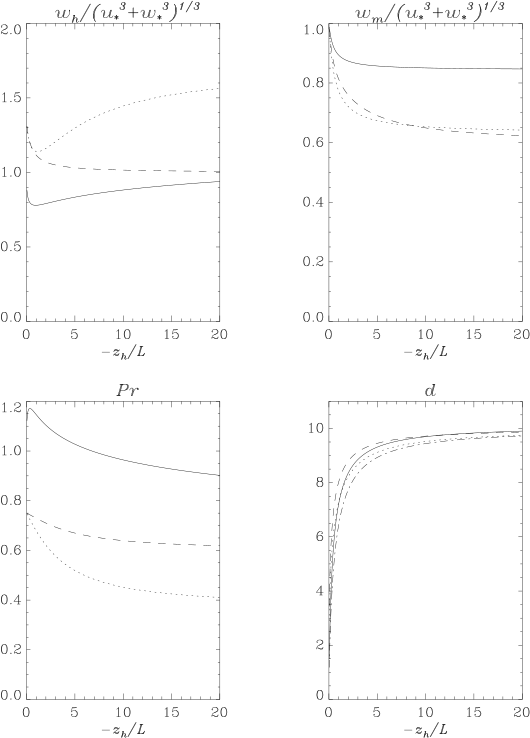
\includegraphics{stab_dep}}
  \caption{Stability dependence of the surface velocity scales,
    Prandtl number (although I hope something is wrong with my coding
    of HB here!) and $d$.  Solid lines are from HB, dotted from the
    standard UM and the dashed from the revised formulation.  The
    dash-dotted line for $d$ is a potential modification, as described
    in the text. }
  \label{fig:stab_dep}
\end{figure}

It is useful to compare the velocity scales in the revised scheme with
those in the standard version, as well as those in
\cite{holtslag93:_local_versus_nonloc_bound_layer}, hereafter HB, on
which the parametrization was originally based.  Recall that HB and
the standard UM set $w_m = (u_*^3 + C_{ws} w_*^3)^{\f{1}{3}}$ and $w_h
= w_m/Pr$, with $C_{ws} = 0.6$ and 0.25, respectively, above the
surface layer.  The convective and neutral limits for $w_h$ and $w_m$
are given in Table~\ref{tab:vscales} and the stability dependencies of
several parameters are shown in Fig.~\ref{fig:stab_dep}.  The
parameter $d$ in Fig.~\ref{fig:stab_dep} contains the stability
dependence of the gradient adjustment parameter:
\begin{equation}
  \gamma_{\chi}= d \f{\wxs}{w_* z_h} 
  \hspace{0.5cm} {\rm with}  \hspace{0.5cm} 
  d^{HB} = 7.2 w_*^2/w_m^2,  \hspace{0.2cm} 
  d^{std} = 6.3 w_*/w_m,  \hspace{0.2cm} 
  d^{rev} = 10 w_*/w_h
  \label{grad_adj}
\end{equation}
The inclusion of an extra $w_*/w_m$ factor in $\gamma_{\chi}$ was a
deliberate change by HB from the original
\cite{troen86:_simpl_model_atmos_bound_layer} formulation on which the
UM was based.  This seems an appealing feature (HB's $\gamma_{\chi}$
will tend to zero as $w_* \rightarrow 0$) and probably should be
considered for the revised scheme (the dash-dotted line in
Fig.~\ref{fig:stab_dep} sets $d^{std} = 10 w_*^2/w_h^2$).  Similarly,
$f_2$ might benefit from an additional factor of the form $(\vsurf +
\vtopc )/ \vsum $ so that it too tends to zero in the neutral limit.
Further analysis of LES and SCM tests will be required to verify this.

Note that the most significant change from the standard UM scheme is
the change to $w_h$ in the convective limit.  Since $\gamma_{\chi}$
remains unchanged in the convective limit, this reduction in $w_h$
will result in a significantly smaller $\wxngs$ for the revised scheme
which gives better agreement against LES.

Compared to the standard scheme, it appears that the revised $\khtop$
is very different.  However, Fig.\ref{fig:new_ksc} shows that this
actually amounts to a small adjustment in the shape.  In addition,
note that the factors $\varepsilon_h^{surf}$ and $\varepsilon_h^{Sc}$
have been removed since the entrainment flux is now carried via the
explicit $f_2$ term.

\begin{figure}[tbh]
  \begin{center}
    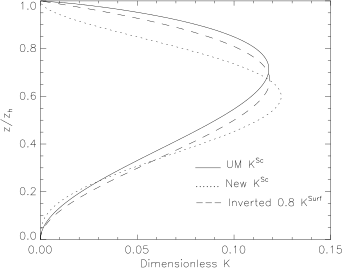
\includegraphics{new_ktop_shape}
    \caption{Standard UM $\khtop$ (solid) and revised (dotted), both
      scaled by $k z_h \vtopo$.  An upside-down version of $\khsurf$
      is also shown (dashed) for comparison.}
    \label{fig:new_ksc}
  \end{center}
\end{figure}

%------------------------------------------------------------------------
% The blended scheme
%------------------------------------------------------------------------
\section{The blended scheme}
\label{sec:blend}

For high resolution simulations, the UM has a Smagorinsky-type
subgrid turbulence scheme, described in \citeumdp{028}. However, this scheme
is only truly applicable for horizontal grid-lengths of order $10$~m,
and any real-world simulation run at lower resolution than this will
inevitably have unresolved scales somewhere in the domain. Rather than
force the user to make an ad-hoc decision about the scales they are
interested in, and thus grid-length at which to switch from using the
boundary-layer parametrization (1D BL) to the subgrid turbulence
scheme (3D Smag), a method for blending the two parametrizations has
been developed. This blend is regime and scale dependent, allowing a
single parametrization to be used across resolutions, including the
completely unresolved/resolved extremes. This blending process is
described in \cite{Boutleetal2014}, which gives some examples of its
use and comparison to simulations using either the 1D BL or 3D Smag
schemes only. Updated technical details from \cite{Boutleetal2014} are
reproduced below.  Several options are available that are selected using 
the switch {\tt blending\_option}.  These all follow the same principles 
but differ in their choice of what should constitute the boundary layer and 
how to treat non-turbulent layers of the atmosphere.

As shown in \cite{Honnertetal2011}, the rate at which turbulent
structures become resolved appears to be different for different
aspects of the flow. For example, moisture fluxes are on a larger
scale than heat or momentum fluxes, and so transition to being
sub-grid at lower resolution. This is just one of many challenges when
creating a truly accurate grey-zone parametrization, and so our aim
here is to start from the simplest possible approach which allows the
model to transition from unresolved to resolved turbulence in a
plausible way, without the user having to decide at which grid-length
to switch from a 1D, non-local, to a 3D, local sub-grid scheme.

Given some function, $W_{1D}$, which tells us how poorly resolved the
turbulence is ($=1$ if unresolved, $=0$ if well resolved), we can use
this to blend between the 1D BL and 3D Smag schemes. Both schemes have
a local Richardson number formulation:
\begin{equation}\label{eq-kri}
  K_\chi(Ri) = l^2 S f_\chi(Ri),
\end{equation}
where $K_\chi$ is the eddy diffusivity, $l$ is the mixing length, $S$
is the wind shear, $f_\chi(Ri)$ is the stability function and $\chi$
represents conserved heat and moisture variables, or momentum. Both
schemes use the same stability function, and both schemes can use the
full 3D shear for $S$. Therefore the only difference is in the mixing
length, which is calculated as
\begin{equation}\label{eq-lblend}
  l_{\rm blend} = W_{1D}l_{\rm bl}+(1-W_{1D})l_{\rm smag},
\end{equation}
where $l_{\rm bl}^{-1} = (\kappa z)^{-1} + \lambda_0^{-1}$ and $l_{\rm
  smag}^{-2} = (\kappa z)^{-2} + (c_s \Delta x)^{-2}$, $\kappa$ is the
von Karman constant and $c_s$ is the Smagorinsky constant. Near the
surface $l_{\rm bl}$ and $l_{\rm smag}$ are identical, but the
asymptotic values are different and this method weights the asymptotic
value according to the weighting of the two schemes. For example, at
$\Delta x=1$~km, $c_s\Delta x=200$~m (for $c_s=0.2$), whereas
$\lambda_0=\max(40\ {\rm m}, 0.15z_h)$, which allows for a small
mixing length in shallow unresolved boundary layers (e.g.~stable
ones).

The \cite{lock00} scheme also contains a non-local component to the
turbulent flux, and this is simply down-weighted by $W_{1D}$ to ensure
that it becomes less significant as the turbulence becomes better
resolved. Therefore the full eddy diffusivity is given by
\begin{equation}
  K_\chi = \max\left[W_{1D}K_\chi^{\rm NL}, K_\chi(Ri)\right],
\end{equation}
where $K_\chi^{\rm NL}$ is the non-local diffusivity and $l$ in
Eq.~\ref{eq-kri} is given by $l_{\rm blend}$ in
Eq.~\ref{eq-lblend}. The turbulent flux is then calculated as
\begin{equation}
  F_\chi=-K_\chi\frac{\partial \chi}{\partial z} + W_{1D}F_\chi^{\rm NL},
\end{equation}
where $F_\chi^{\rm NL}$ is the non-local flux. Therefore when
$W_{1D}=1$, the scheme of \cite{lock00} is recovered, whilst with
$W_{1D}=0$ the Smagorinsky-type scheme is recovered.

Now we need to define the function $W_{1D}$ to blend the schemes. Within the
boundary layer this is based on the turbulent kinetic energy partitioning 
given by \cite{Honnertetal2011}. We choose the TKE
partitioning because it is most closely linked to the eddy diffusivity
we are trying to parametrize (for example a TKE based scheme would
calculate the eddy diffusivity from the TKE), and simplify the
function slightly, using
\begin{equation}\label{eq-tanh}
  W_{1D} = 1 - \tanh\left(\beta\frac{z_{\rm turb}}{\Delta x}\right)\max\left[0,\min\left[1,r_f\left(l_0-\frac{\Delta x}{z_{\rm turb}}\right)\right] \right],
\end{equation}
where $z_{\rm turb}$ is the appropriate lengthscale of the turbulence,
$\beta$ is a scaling parameter which controls the speed of the
transition from unresolved to resolved
turbulence, $r_f=\frac{1}{l_0-l_1}$, $l_0=4$ and $l_1=0.25$ (N.~B.~this
formula is slightly modified from that given in \cite[]{Boutleetal2014}).
\cite{Malavelleetal2014} demonstrated that this scaling
method was applicable to any type of unstable boundary layer given an
appropriate choice of $z_{\rm turb}$.  In \cite{Boutleetal2014} this 
functional form was applied everywhere, adjusting the values of 
$z_{\rm turb}$ and $\beta$ depending on the regime.  
The max function is present to force the lowest resolution simulations 
to just use the 1D mixing scheme.  An alternative approach that differs 
above the boundary layer is described below.

The simplest case is for a well-mixed boundary layer, where the
appropriate lengthscale is the boundary-layer depth (inversion
height). Therefore we set $z_{\rm turb}=z_h$, which is broadly
consistent with \cite{Malavelleetal2014}, and choose $\beta=\beta_{\rm
  bl}=0.15$ to give the best match of our function to that of
\cite{Honnertetal2011}. These functions are shown in
Figure~\ref{fig-blend}(a) and are only dissimilar for small $\Delta
x$, where Eq.~\ref{eq-tanh} tends to zero faster. This is by choice,
to force the highest resolution simulations to use the 3D turbulence
scheme.
\begin{figure}[tbh]
  \centering
  \noindent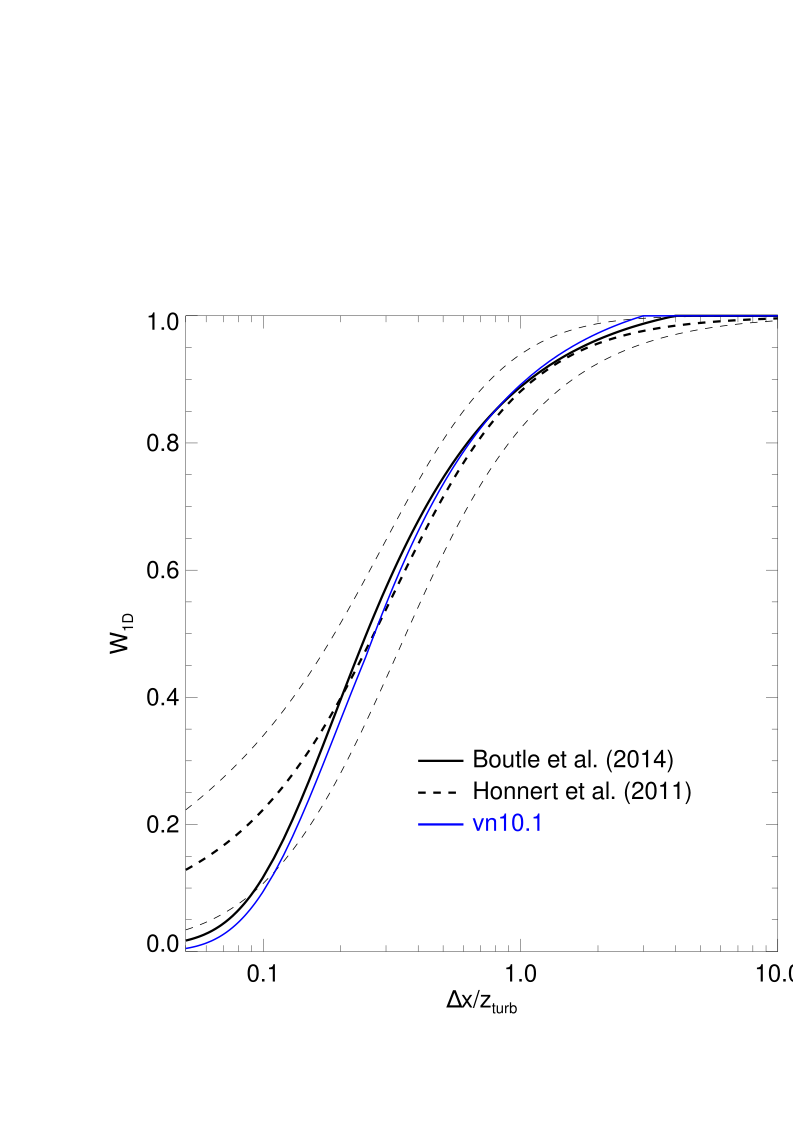
\includegraphics[width=0.49\columnwidth]{honnert_vs_tanh.eps}
  \noindent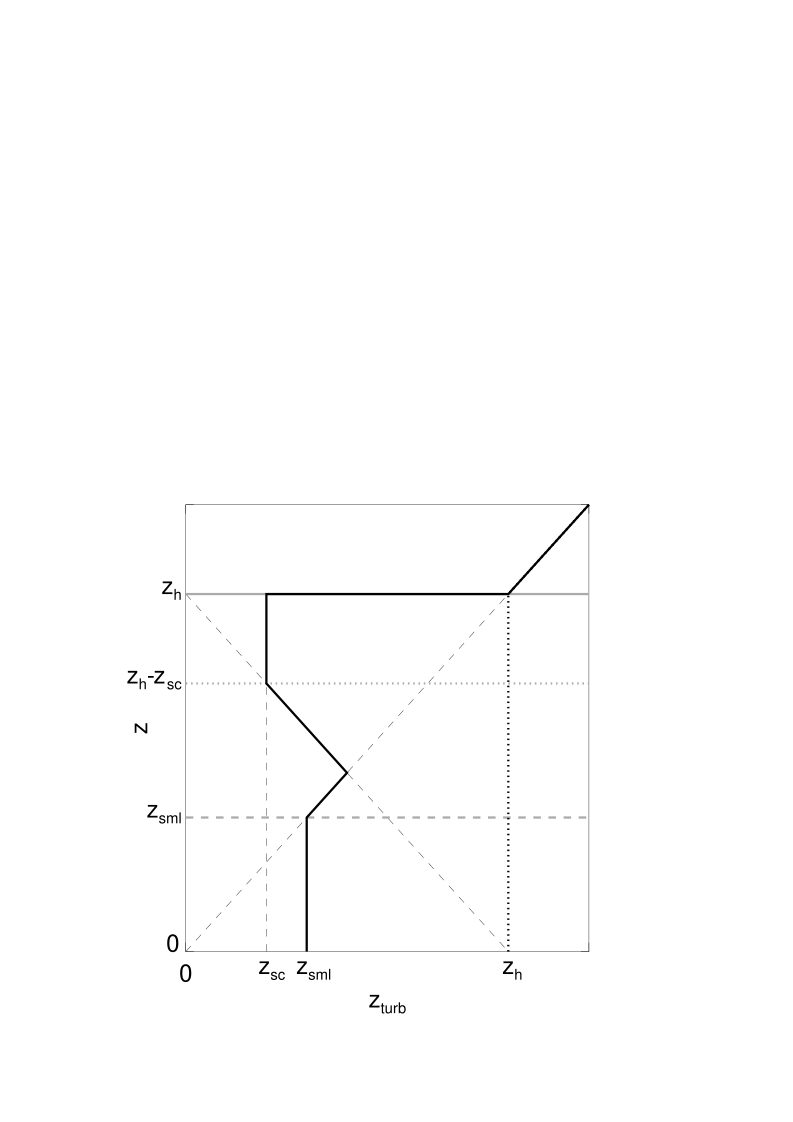
\includegraphics[width=0.49\columnwidth]{zturb_schem.eps}
  \caption{(a) Weighting for the 1D boundary-layer scheme as a
    function of $\Delta x/z_{\rm turb}$, showing the function of
    Equation~\ref{eq-tanh} (blue solid), the equation in
    \cite{Boutleetal2014} (black solid) and the TKE partitioning of
    \cite{Honnertetal2011} (mean thick dashed, 5th/95th percentiles
    thin dashed). (b) Schematic showing the calculation of $z_{\rm
      turb}$ used in Eq.~\ref{eq-tanh} for a well-mixed layer (black
    dotted) and a decoupled cloud layer (black solid).}
  \label{fig-blend}
\end{figure}

One of the key benefits of the \cite{lock00} scheme is its ability to
represent decoupled stratocumulus layers, and this is a feature which
needs to be maintained in the blended scheme. Physically they are
similar to well-mixed surface driven boundary layers, and the
\cite{lock00} scheme parametrizes them as such. The appropriate length
scale is now the decoupled cloud mixed layer depth, $z_{\rm sc}$
\cite[i.e.~the depth through which a negatively buoyant parcel
released at cloud top would descend,][]{lock01}. In this case, below
the decoupled cloud top we set
\begin{equation}\label{zturb_dsc}
  z_{\rm turb}=\min\left[\max\left(z,z_{\rm sml}\right),\max\left(z_{\rm sc},z_h-z\right)\right],
\end{equation}
where $z_{\rm sml}$ is the depth of the surface-based mixed layer
\cite[i.e.~the depth through which a positively buoyant parcel
released at the surface would ascend,][]{lock00}. This is shown
schematically in Figure~\ref{fig-blend}(b), and ensures that $W_{1D}$
has a high value in the poorly resolved surface mixed layer and cloud
layer, and a lower value in between those layers. Again, this choice
of $z_{\rm turb}$ is broadly consistent with the analysis of decoupled
stratocumulus LES presented by \cite{Malavelleetal2014}.  Finally, 
\cite{Honnertetal2011} also included shallow cumulus simulations and 
showed that the relevent length scale there was the cloud top height.  Most 
of the {\tt blending\_option} choices apply this to all regimes diagnosed 
as cumulus-capped (see section~\ref{sec:types}) but alternatively 
({\tt blending\_option}$=$4) this can be restricted to strictly shallow 
cumulus clouds, defined as contiguously cloudy levels (cloud fraction 
greater than SC\_CFTOL) with cloud top height below input parameter 
{\tt shallow\_cu\_maxtop}.  Note that the diagnosis of shallow cumulus 
from the diagnosis parcel ascent (that was used to identify a cumulus regime) 
was found frequently to indicate deep convection even when the resolved 
clouds were shallow because the diagnosis parcel, being undilute, would 
penetrate to the tropopause.  However, having decided the regime is shallow 
convection, we do still set $z_{\rm turb}$ to the diagnosis parcel top height 
because, for current km-scale configurations (without a cumulus convection 
parametrization), it was found that the resulting stronger parametrized 
vertical mixing was beneficial for the development of the convection, and 
that without this a widespread stratiform cloud layer could develop instead.

Above the boundary layer top, \cite{Boutleetal2014} aimed for any free 
atmospheric mixing to be done by the 3D Smagorinsky scheme. Therefore, above
the boundary layer top they use $z$ as the appropriate length scale, and in 
general take $z_{\rm turb}$ in Eq.~\ref{eq-tanh} as the greater of that defined 
by (\ref{zturb_dsc}) and $z$. However, this did not give a particularly 
fast transition using the value of $\beta_{\rm  bl}$, therefore they used 
$\beta_{\rm fa}=1$ at a height well above the boundary layer 
($z_{\rm fa}=z_h+1$~km), and transitioned between these regimes linearly using
\begin{equation}
  \beta = \beta_{\rm bl}\frac{z_{\rm fa}-z}{z_{\rm fa}-z_h} + 
          \beta_{\rm fa}\frac{z-z_h}{z_{\rm fa}-z_h}
\end{equation}
However, because the above method still uses (\ref{eq-tanh}), which depends on 
$z_{\rm turb}/\Delta x$, the rate of transition to 3D Smagorinsky with height 
above the boundary layer varies in an undesirable way with grid size.  It 
might be considered more logical to think of non-turbulent regions of the free 
troposphere as unresolved turbulence and so revert to the 1D mixing scheme 
there.  An alternative treatment({\tt blending\_option}$=$3 or 4), then, is to 
increase $W_{1D}$ above the boundary layer top smoothly, to reach unity by 
some physical height $z_{\rm fa}$, to be independent of both horizontal and 
vertical grid sizes.  For $z_{\rm turb} < z < z_{\rm fa}$, then, we set
\begin{equation}
  W_{1D} = 1 + \frac{1}{2} \left( W_{1D}|_{z=z_{\rm turb}} - 1 \right)
    \left[ 1 + {\rm cos}\left( \pi \, \frac{z-z_{\rm turb}}{z_{\rm fa}-z_{\rm turb}}
                     \right) \right]
\end{equation}
The cosine term in square brackets transitions smoothly from 2 at 
$z=z_{\rm turb}$ to zero at $z_{fa}$ where, although somewhat 
arbitrary, $z_{\rm fa} = {\rm min}(2 z_{\rm turb}, z_{\rm turb}+1 {\rm km})$.  
The former term ensures the transition is well above any shallow boundary 
layers while the latter that it does not drift far into the free atmosphere.  
In addition, within any layers identified as turbulent, through having 
subcritical $Ri$, $z_{\rm turb}$ is set to the layer depth, in the same way 
as is done for decoupled stratocumulus in (\ref{zturb_dsc}).

For current operational convection-permitting model grid sizes (1.5 km
in the UKV), the representation of cumulus convection remains a
challenge.  One option is to include a grey-zone convection
parametrization, described in the documentation of that scheme 
(see \citeumdp{027}).  Tests in the UKV, though, showed some
detriment to the spin-up of resolved scale convection (as well as
somewhat poor discrimination of precipitating versus non-precipitating
parametrized convection) that led to the development of an alternative
strategy, namely to abandon the blended turbulence scheme when pure
cumulus convection was diagnosed and leave the representation of
cumulus entirely to the resolved scales.  This option 
({\tt blending\_option}$=$2) is also now discouraged.

%------------------------------------------------------------------------
% ENTRAINMENT
%------------------------------------------------------------------------
\section{Entrainment fluxes}
\label{sec:entr}

{\bf Summary}: parametrized entrainment fluxes (at the top of mixed
layers) are specified for momentum through an eddy-diffusivity, as
described in section~\ref{sec:ent_K}.  For scalar variables, if the
inversion is sufficiently sharp so as to be unresolved, the ideal is
to specify the entrainment fluxes explicitly, as described in
section~\ref{sec:ent_flux}, based on the subgrid inversion diagnosis
described in section~\ref{sec:sginv}.  Further details can be found in
\cite{lock01}.  If the profiles are such that the inversion is sharp
but a subgrid inversion cannot be diagnosed, an eddy-diffusivity
similar to that for momentum is used (see section~\ref{sec:ent_K}).
If the inversion is thick enough to be resolved then an eddy
diffusivity profile is constructed across the inversion (see
section~\ref{sec:entr_prof}) for both scalars and momentum fields.
For tracer variables (scalars other than $\thetal$ and $q_t$), the
entrainment fluxes are specified using an equivalent eddy-diffusivity,
as described in section~\ref{sec:ent_K_flux}.  Note that, as indicated
below, several aspects of the implementation of entrainment fluxes
were revised at the 9C scheme and these are documented separately.

The parametrization of the entrainment rate, $w_e$ (given, in the
absence of subsidence, by the rate of rise of the inversion), can be
written (using the notation given in appendix~\ref{app:vscales})
\begin{equation}
  w_e =  \frac{ A_1 \, \vsum / \zml + g \tilde{\beta_T} \tilde{\alpha_t} 
    \Delta_\radf }
  {\Delta b + c_T \vsumo^2/\zml }
  \label{we_parm}
\end{equation}
where $ \vsum = \vheat + \vrad + \vbr + A_2 u_*^3 $.  The constant
$A_1$ is given a value 0.23, as in \cite{lock98}, and $A_1*A_2=5$, as
in \cite{driedonks1982}.  To allow for weak inversions, the
\cite{zilitinkevich1975} correction is included in (\ref{we_parm})
with the constant, $c_T=1$.  A further parametrization for $\alpha_t$,
which is the fraction of the cloud-top radiative divergence
($\Delta_\radf $, in Kms$^{-1}$) that occurs across the
horizontally-averaged inversion in the LES, can be written
\begin{equation*}
  \alpha_t = 1 - \exp{ \left\{-\Delta z_i / (2 L_{rad})\right\} }
\end{equation*}
where the thickness of the inversion is parametrized as $\Delta z_i =
\mbox{min}[\vsumo^2/\Delta b, 100]$ and $L_{rad}$ is a depth-scale for
the radiatively-cooled layer (taken to be 15 $\times
\,\mbox{max}[200/z_c, 1]$, where $z_c$ is the cloud depth).  To allow
for a feedback with forcing of entrainment by buoyancy reversal (see
appendix~\ref{app:vscales}), $\tilde{\alpha_t} = \alpha_t+ Br
(1-\alpha_t) $.  following \cite{lock98} and \cite{lock09:_factor}.
The calculation of the other quantities required for (\ref{we_parm})
is described in appendix \ref{app:vscales}.  At some point during the
transition to a decoupled boundary layer the surface-driven
entrainment terms (the terms in (\ref{we_parm}) proportional to
$\vheat$ and $u_*$) will no longer contribute to entrainment at cloud
top, because the two layers will have become entirely decoupled.  If
the {\tt entr\_smooth\_dec} switch is on then the surface contribution
to the parametrized entrainment at \zhsc is decreased linearly as the
$\thetavl$ difference between NTDSC and NTML increases from 0.5 to 1K.
The flag, COUPLED, is set to true and \zhsc is used as the mixed-layer
depth in (\ref{we_parm}) as long as any surface-driven entrainment
remains.  If the {\tt entr\_smooth\_dec} switch is off then this
transition is discontinuous at a $\thetavl$ difference of 0.5K.

It should be noted that (\ref{we_parm}) takes no account of wind shear
anywhere other than at the surface.  How to quantify the shear
generation of turbulence in DSC layers is not known.  The direct
impact of shear across the inversion is thought to be simply to
diffuse the inversion in the vertical --- this wind shear will
contribute little to the mixed layer TKE and so can not contribute to
the full process of mixing across the inversion and down into the
mixed layer that is entrainment.  However, important interactions
between wind shear across inversions and cloud-top radiative cooling
have been observed that are not yet accounted for in the UM.

The least well-determined part of (\ref{we_parm}) is the constant
$A_2$ --- the constant in the Zilitinkevich correction, $c_T$, is also
approximate but is included to limit the growth of layers capped by
weak inversions and for numerical safety.  A further limit is applied
to the value of $w_e$ determined by (\ref{we_parm}) such that the
inversion cannot rise by more than one grid-level in a timestep.  With
current vertical resolutions and timesteps this is not a serious
restriction.  The constants $A_1$ and $A_{\rm br}$ appeared to be
determined within 10-20 \% in \cite{lock98}, although only solid cloud
sheets were simulated (as discussed further in
appendix~\ref{app:vscales}).  Similarly the parametrizations of
$\alpha_t$ and $\Delta z_i$ were found to be accurate but the
parameter $L_{rad}$ is currently only crudely represented in the UM.

\subsection{Specification of entrainment fluxes in the 9B scheme}
\label{sec:ent_flux}
Note that the 9C scheme (see next section) differs by generalising the
approach to include all processes operating in the inversion
grid-level, rather than just radiation.

If it is assumed that the turbulent fluxes reduce from their extremum
at $z=z_i$ (the `entrainment' fluxes) to zero at $z=h$ a small
distance above, then $ \wthlzi = - w_e \Delta \thetal + \radf|_h -
\radf|_{z_i}$, so that
\begin{eqnarray}
  {\cal H}|_{z_i} & =& - w_e \Delta \thetal + \radfnet|_h \nonumber\\
  \wqtzi         & =& - w_e \Delta q_t
\end{eqnarray}
\label{discinv}
where the total heat flux ${\cal H} = \wthl + \radfnet$ and $\radfnet
= \radf - \radf|_{\zbaseq}$.  The net radiative flux relative to the
base of the mixed layers is simply calculated as
\begin{equation*}
  \radfnet|_{z_{k+\frac{1}{2}}} = \sum_{k=\nbdsc}^{k} \mbox{max}\left[ 
    - \Delta_{k+\frac{1}{2}} z \, {\cal S}_\radf(k), \,0 \right]
\end{equation*}
where NBDSC$=1$ in SMLs, ${\cal S}_\radf$ are the temperature
increments (in Ks$^{-1}$) from the radiation scheme and $\radfnet|_h$
is estimated by extrapolating down from $\radf|_{z_{\ntml+\frac{3}{2}}
}$ using the flux-divergence in grid-level NTML$+2$ (and similarly for
DSC layers).

The thermodynamic variables' entrainment fluxes, then, are imposed
nominally at the subgrid inversion height ($z_i=$ \zh and/or \zhsc),
diagnosed as described in section~\ref{sec:sginv}.  The required
grid-level fluxes (at $z_{\ntdsc+\frac{1}{2}}$, for example) are then
estimated using linear interpolation of ${\cal H}$ and $\wqt$ between
\zhsc and the base of the mixed layer:
\begin{eqnarray}
  \wthl|_{ z_{\ntdsc+\frac{1}{2}} } & =& \wthl|_{\zbaseq} 
  - \frac{ z'_{\ntdsc+\frac{1}{2}} }{\zml}
  \left( \tilde{w_e} \Delta \thetal + \wthl|_{\zbaseq} - \radfnet|_{h} \right)
  - \radfnet|_{ z_{\ntdsc+\frac{1}{2}} } \nonumber\\
  \wqt|_{ z_{\ntdsc+\frac{1}{2}} } & =& \wqt|_{\zbaseq} 
  - \frac{ z'_{\ntdsc+\frac{1}{2}} }{\zml} 
  \left( \tilde{w_e} \Delta q_t + \wqt|_{\zbaseq} \right)
\end{eqnarray}
\label{fluxinterp}
where $z' = z-\zbaseq$, and similarly for the SML entrainment fluxes
(at $z=z_{\ntml+\frac{1}{2}}$).  The turbulent fluxes at the base of
the mixed layer are assumed zero except for the SML where the surface
fluxes are used.  This interpolation is illustrated for a SML in
Fig.~\ref{fig:fluxinterp}.
\begin{figure}[tbh]
  \centering
  \scalebox{1.0}{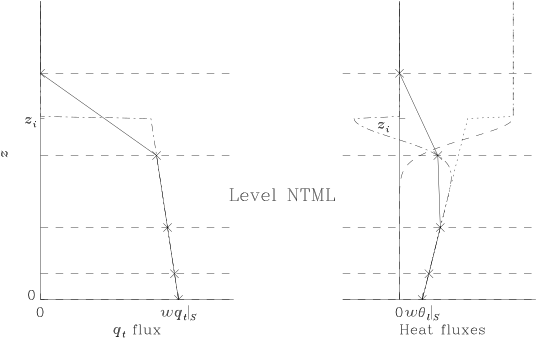
\includegraphics{subsent_fig7}}
  \captionarb{Idealised profiles of (a) $\wqt$ (dash-dotted line) and
    (b) ${\cal H}$ (dotted line), $\wthl$ (dash-dotted) and $F$
    (dashed).  The continuous lines are the turbulent fluxes on the
    model grid indicated by the dashed horizontal lines.}
  \label{fig:fluxinterp}
\end{figure}
Note that, because (\ref{fluxinterp}) includes an explicit balance
between the turbulent and radiative fluxes for $\wthl$, it is not
possible to parametrize the entrainment fluxes through a single $K_h$
for both $\wthl$ and $\wqt$.  Furthermore, the radiative forcing of
turbulence in the mixed layer is fixed through the timestep and so it
is consistent to assume the entrainment fluxes (at $z_i$) are also
fixed.  Hence (\ref{fluxinterp}) are implemented explicitly, rather
than via an eddy-diffusivity.  This is discussed further, with
reference to tracer fluxes, in section~\ref{sec:ent_K_flux}.

In order to allow for the long timesteps used in NWP and to facilitate
movement of the subgrid inversion across grid-levels within a
timestep, the parametrization of $w_e$ and the model's subsidence
velocity, $w_S|_{z_i}$, are used to calculate $z_i$ at the next
time-level ($z_i^{n+1}$).  Currently, the latter is found by linear
interpolation to $z_i$ and both are assumed constant in time.  If
$z_i^{n+1} < z_{\ntdsc +\frac{1}{2}}$, then the entrainment fluxes
there (given by (\ref{fluxinterp})) are multiplied by the fraction of
the timestep that $z_i$ was above this grid-level, namely
$(z_i-z_{\ntdsc +\frac{1}{2}})/(z_i - z_i^{n+1}) $.  The full
entrainment flux at grid-level NTDSC$-\frac{1}{2}$ must then also be
specified, given by (\ref{fluxinterp}) with $z_{\ntdsc + \frac{1}{2}}$
replaced by $z_{\ntdsc - \frac{1}{2}}$.  If $z_i$ rises above
$z_{\ntdsc+\frac{3}{2}}$, the entrainment flux is specified only at
this higher grid-level (multiplied by the fraction of the timestep
that $z_i$ is above this half-level) and the values of the mixed-layer
$K$ profiles are used in half-level NTDSC$+\frac{1}{2}$ (these will be
non-zero because $z_i>z_{\ntdsc + \frac{1}{2}}$).  Wherever the
entrainment fluxes are specified explicitly, the eddy-diffusivities
(both non-local and local) are set to zero.  Also, the mean value of
$z_i$ during the timestep is used in (\ref{fluxinterp}) in order best
to approximate the mean flux gradient across the mixed layer.

Finally, the entrainment flux is adjusted to allow for numerical
entrainment arising from the model's resolved vertical advection (as
discussed in \cite{lock01}).  This is performed at whichever
grid-level the entrainment fluxes are specified, to allow for any
entrainment implied by a $\thetal$ subsidence increment, $\Theta^{\rm
  S}$ (Ks$^{-1}$), at the model grid-level below.  The subsidence
increments could be obtained directly in the SCM but in the full 3D UM
advection increments are dominated by the horizontal component.  The
subsidence increments are calculated, therefore, from the vertical
velocity field using first order upwind advection (it would clearly be
preferable to use the model's actual vertical advection algorithm in
the GCM although the errors incurred in this diagnostic calculation
should not be very significant).  The interpolated entrainment fluxes
given by (\ref{fluxinterp}) are therefore calculated not using $w_e$
but using an entrainment velocity, $\tilde{w_e}$, that is reduced to
allow for any subsidence increments applied to the grid-level below
the entrainment flux.  To take the case of $z_{\ntdsc+\frac{1}{2}} <
z_i^{n+1} < z_{\ntdsc+\frac{3}{2}}$ as an example, this reduced
entrainment velocity is given by
\begin{equation*}
  \tilde{w_e} = w_e + \tilde{w_S} 
\end{equation*}
with $\tilde{w_e}$ constrained to lie between 0 and $w_e$ and 
\begin{equation}
  \tilde{w_S} = - \, \frac{ \Theta^{\rm S}_{\ntml}
    ( \Delta_{\ntml+\frac{1}{2}} z ) }
  { \Delta \thetal }
  \label{we_num}
\end{equation}

\subsubsection{Diagnosis of a sub-grid inversion}
\label{sec:sginv}

The profile of $\thetavl$ is used to diagnose the height of a
discontinuous inversion because it is approximately conserved under
adiabatic vertical motion and is equal to the virtual potential
temperature, $\theta_v$, in the absence of cloud.  This should ensure
it is monotonically increasing with height in the statically stable
free-troposphere of a GCM.  If $\thetavl$ does not increase
monotonically between grid-levels NTML and NTML+2 (or NTDSC and
NTDSC+2), then entrainment fluxes are simply specified via
(\ref{khent}) and none of the coupling with subsidence or radiation
described above is attempted (the local scheme is also currently not
set to zero above NTML or NTDSC when this occurs to allow it to
diffuse out this static instability).

\begin{figure}[tbh]
  \centering
  \scalebox{1.0}{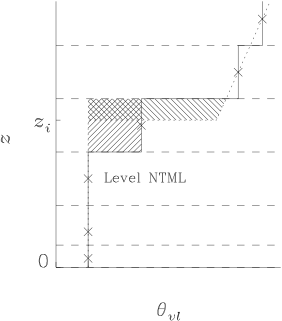
\includegraphics{nbldoc_zidiag}}
  \captionarb{Schematic illustrating the assumptions behind the
    subgrid diagnosis of $z_i$.}
  \label{zi_diag}
\end{figure}
Having identified the model grid-level at the top of the well-mixed
layer (either level NTML from the parcel ascent, as described in
section~\ref{sec:adiapar}, or NTDSC for DSC layers, see section
\ref{sec:decouple}--- the analysis is the same for both), the
grid-level above is designated the inversion level within which the
diagnosis of a subgrid $z_i$ will be made.  It is assumed that
$\thetavl$ in grid-level NTML$+1$ represents a cell-average value.
Thus, $z_i$ can be calculated by assuming that the integral of
$\thetavl$ over grid-level NTML$+1$ for the model and for a profile
with a discontinuous inversion at $z_i$ are equal, as illustrated by
the hatched areas in Fig.~\ref{zi_diag}.  To calculate the integral of
the discontinuous profile, the lapse rate of $\thetavl$ between
grid-levels NTML$-1$ and $NTML$, $\gammaml$, is extended up to $z_i$,
while the stable lapse in the free atmosphere, between grid-levels
NTML$+2$ and NTML$+3$, $\gammafa$, is extrapolated down.  Equating
these areas gives a quadratic equation in $\Delta z_{disc} =
z_{\ntml+\frac{3}{2}} - z_i$ which can be written
\begin{equation}
  a (\Delta z_{disc})^2  + b \ \Delta z_{disc} +c =0 
\label{zi_interp}
\end{equation}
The coefficients are given by
\begin{eqnarray*}
  a & =& 0.5 (\gammafa - \gammaml)   \\
  b & =& - \left( {\thetavl}_{\ntml+2}
    - \gammafa (z_{\ntml+2}-z_{\ntml+\frac{3}{2}}) \right)
  + \left( {\thetavl}_{\ntml}
    + \gammaml (z_{\ntml+\frac{3}{2}}-z_{\ntml}) \right)  \\
  c & =& (z_{\ntml+\frac{3}{2}}-z_{\ntml+\frac{1}{2}})
  \left( {\thetavl}_{\ntml+1} -
    \left( {\thetavl}_{\ntml} +
      \gammaml \left(
        \frac{1}{2}(z_{\ntml+\frac{1}{2}}+z_{\ntml+\frac{3}{2}})
        -z_{\ntml} \right)     \right)
  \right)  \\
\end{eqnarray*}

Clearly, care must be taken to ensure that $z_i$ is not only
well-defined but also sensible (for example, as a rising inversion
encounters more or less stable regions above).  If $b>0$ this suggests
the estimated lapse rates are inappropriate and these are therefore
set to zero and (\ref{zi_interp}) is recalculated.  The case $c<0$
suggests the grid-level designated as the inversion level should have
been considered as part of the mixed layer and so $z_i$ is set to be
fractionally below $z_{\ntml+\frac{3}{2}}$ (\mbox{i.e.}, as high as
possible without attempting to diagnose a subgrid $z_i$ in grid-level
NTML$+2$).  If $b^2-4ac<0$ the quadratic equation has no real roots.
In this instance $z_i$ is set to fractionally below
$z_{\ntml+\frac{1}{2}}$ and NTML (and therefore the eddy-diffusivity
profiles) is lowered by a grid-level.  In all other circumstances, the
required root is then $\Delta z_{disc} = (-b - (b^2-4ac)^{1/2}
)/(2a)$; the other root will either be larger or negative (if $a<0$).

In addition, from variations seen in $z_i$ during single-column model
simulations, the error in $\Delta z_{disc}$ is estimated to be around
10\% of the vertical resolution, $\Delta_{\ntml+\frac{3}{2}} z$.
Accordingly, if $z_i$ is diagnosed as being less than
$z_{\ntml+\frac{1}{2}} + 0.1 \, \Delta_{\ntml+\frac{3}{2}} z$, NTML is
lowered a grid-level and $z_i$ is set fractionally below
$z_{\ntml+\frac{1}{2}}$.  This small distance below the grid-level is
taken to be $(\Delta t/2) \times 10^{-4}$ so that, were a small rate
of rise of $z_i$ (of $10^{-4}$ ms$^{-1}$, say) to be diagnosed, then
$z_i$ would spend at least half the timestep (of length $\Delta t$) in
the next grid-level up.  The specified fluxes would then contribute
significantly to that grid-level's evolution.  Conversely, if $z_i$ is
subsiding, this technique allows the inversion to drop down a
grid-level without requiring this to be detected by the initial parcel
ascent.
 
Having calculated $z_i$, the discontinuous jumps in $\thetal$ and
$q_t$ that are used in the entrainment calculation are calculated from
similar integral assumptions:
\begin{equation}
  \Delta \chi = \left( {\chi}_{\ntml+1} - {\chi}_{\ntml} \right) \,
  \frac{ z_{\ntml+\frac{3}{2}} - z_{\ntml+\frac{1}{2}} }
  { z_{\ntml+\frac{3}{2}} - z_i }
\label{dqt_disc}
\end{equation}
with $\chi = \thetal$ and $q_t$.  Note that the lapse rate above the
inversion has been ignored as there is no guarantee of monotonicity in
$q_t$ in the atmosphere above the inversion.  In addition,
(\ref{dqt_disc}) will become increasingly inaccurate as $z_i$ tends to
$z_{\ntml+\frac{3}{2}}$ (and so ${\chi}_{\ntml+1}$ approaches
${\chi}_{\ntml}$).  Consequently, if the fraction on the right hand
side of (\ref{dqt_disc}) is greater than 10, double grid-level jumps
are used (\mbox{i.e.}, $\Delta \chi = {\chi}_{\ntml+2} -
{\chi}_{\ntml} $).  Finally, note that (\ref{dqt_disc}) implicitly
assumes the structure of the $\thetal$ and $q_t$ profiles across the
inversion grid-level are consistent with the diagnosed $z_i$.  This is
very unlikely to be the case, for example, when running from an
analysis so the 9C scheme uses what has been found to be a more robust
algorithm, see the separate documentation.

It would clearly be advantageous to pass knowledge of this subgrid
inversion structure to other parametrizations in the UM, particularly
the cloud scheme as currently the cloud fraction in level NTML$+1$ is
essentially meaningless (being diagnosed from a mixture of cloudy
boundary layer air and typically very dry free tropospheric air).

\subsection{Specification of entrainment fluxes across sharp inversions in the 9C scheme}
\label{sec:ent_flux_9c}

As described in section~\ref{sec:ent_flux}, when the capping inversion
is thinner than the model vertical grid it is important for the
entrainment flux implementation that the subsidence increments are
realistically and consistently distributed between the inversion
grid-level and the mixed layer.  Rather than work with the increments
themselves, though, a more robust solution is to couple the subsidence
and turbulent fluxes across the inversion, exactly analogously to the
coupling of turbulent and radiative fluxes.  This allows the total
tendency of the inversion grid-level to be linked to whether the
inversion should be rising or falling (determined from the balance
between the parametrized entrainment rate, $w_e$, and the large-scale
vertical velocity evaluated at the inversion, $w|_{z_h}$).

\begin{figure}[p]
  \centering
  \scalebox{1}{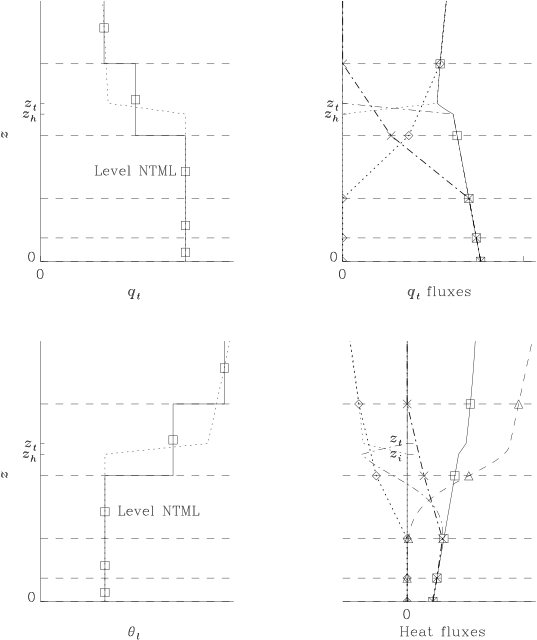
\includegraphics{ideal_revflux}}
  \caption{Subgrid (lines) and model (symbols) profiles and fluxes of,
    top row, $q_t$ and, bottom row, $\thetal$: turbulent fluxes
    (dash-dotted, crosses), subsidence fluxes (dotted, diamonds),
    radiative flux (dashed, triangles) and total flux (solid,
    squares).}
  \label{fig:rev_fluxes}
\end{figure}
An idealised subgrid total flux profile is constructed from the
parametrized entrainment flux and the increments from radiation,
precipitation and subsidence, assuming a well-mixed boundary layer
capped by a diagnosed subgrid inversion.  The crucial step is to
ensure that the total flux on the model entrainment grid-level equals
the idealised total flux profile interpolated to that level.  Consider
the example illustrated in Fig.~\ref{fig:rev_fluxes} of a well-mixed
boundary layer up to $\theta$-level $\ntml$.  For the subgrid $q_t$
profiles, the turbulent flux divergence generates a moistening across
the inversion while subsidence generates drying.  For this example it
has been assumed the entrainment rate is slightly larger than the
subsidence velocity at the inversion and so overall there is a weak
moistening relative to the mixed layer (the total flux gradient is
more negative across the inversion than in the mixed layer),
consistent with the rising tendency of the inversion.  For the model,
the subsidence flux-divergence associated with the inversion is split
across levels $\ntml$ and $\ntml+1$.  To keep the {\em net} moistening
of the model's boundary layer and inversion consistent with the total
subgrid flux profile, the model's entrainment flux at $\ntml+1/2$
(shown by the cross in Fig.~\ref{fig:rev_fluxes}) must be found by
subtracting the subsidence flux at $\ntml+1/2$ (diamond) from the
total flux interpolated to $\ntml+1/2$ (square).  Exactly the same
arguments follow for the $\thetal$ fluxes except that the situation is
complicated by the addition of the radiative flux.

The above arguments can be generalised as follows.  Writing $\fxtot$
as the total flux of a conserved variable $\chi$ ($=q_t$ or $\thetal$)
and $\fxntp$ as the flux from physics sources other than turbulence
(\mbox{i.e.}, radiation, $\fx^{rad}$, in the above examples, but
including precipitation fluxes, $\fx^{ppn}$, in the full model) and
$\fx^{subs}$ as the flux from resolved scale subsidence, the total
flux at the subgrid inversion height is given by:
\begin{equation}
  \fxtot|_{z_h} = - w_e \Delta \chi + \fxntp|_{z_t} + \fx^{subs}|_{z_h}
  \label{fxtot_zi}
\end{equation}
As in section~\ref{sec:ent_flux}, (\ref{fxtot_zi}) is derived by
integrating the conservation equation for $\chi$ over an inversion in
which jumps occur over a thin layer with base at a height $z_h$ and
top at $z_t$ (in the UM, the inversion is assumed to be
infinitesimally thin so that $z_t=z_h$).  This integration gives $ -
w_e \Delta \chi = \wx|_{z_h} -(\fxntp|_{z_t}-\fxntp|_{z_h})$.
\cite{lock99} related the non-turbulent flux divergence,
$\fxntp|_{z_t}-\fxntp|_{z_h}$, to radiative cooling occurring within
undulations of the cloudy boundary layer top.  Similar considerations
need to be borne in mind when calculating all the non-turbulent fluxes
in (\ref{fxtot_zi}).  First, the radiative flux is extrapolated down
from $\ntml+\frac{3}{2}$ to $z=z_t$ using the divergence in the
grid-level above the inversion as representative of the
free-atmospheric divergence.  Second, since the microphysical flux is
generated within the cloud, $\fx^{ppn}|_{z_t} =
{\fx}^{ppn}_{\ntml+\frac{3}{2}}$.  Finally, the subsidence
flux-divergence across level $\ntml$ and $\ntml+1$ is assumed to be
associated with the inversion so ${\fx}^{Subs}|_{z_h} =
{\fx}^{Subs}_{\ntml-\frac{1}{2}}$.  Thus, the finite-difference form
of (\ref{fxtot_zi}) becomes \beqn \fxtot|_{z_h} = - w_e \Delta \chi +
\fx^{rad}|_{z_t} + {\fx}^{ppn}_{\ntml+\frac{3}{2}} +
{\fx}^{subs}_{\ntml-\frac{1}{2}}
\label{fxtot_zi_fd}
\eeqn

Then, assuming a linear profile of $\fxtot$ in the mixed layer,
interpolating the total flux to the inversion flux grid-level gives
\begin{equation}
  \fxtot|_{ \ntml+\frac{1}{2} } = \fxtot|_{\zbaseq} + 
  \frac{ z'_{\ntml+\frac{1}{2}} }{\zml} 
  \left( \fxtot|_{z_h} - \fxtot|_{\zbaseq} \right)
  \label{fxtot_interp}
\end{equation}
where $z'$ ($=z-\zbaseq$) is height above the base of the mixed layer
at $z=\zbaseq$.  Finally, the grid-level turbulent entrainment flux is
given by:
\begin{equation}
  \wx|_{ \ntml+\frac{1}{2} } = \fxtot|_{ \ntml+\frac{1}{2} } 
                       - \fxnt|_{ \ntml+\frac{1}{2} }
  \label{rev_entflux}
\end{equation}
This revised algorithm has several advantages over the previous.
Firstly, the fluxes for $q_t$ and $\thetal$ are coupled independently,
whereas in the 9B version the coupling with subsidence was estimated
using only the $\thetal$ increments in order to calculate
$\tilde{w_e}$ in \ref{we_num}.  Secondly, this method makes it much
simpler to include all processes, and precipitation in particular, in
a consistent manner.  Thirdly, since the total grid-level flux,
$\fxtot|_{\ntml+\frac{1}{2}}$ in (\ref{fxtot_interp}), is used to
calculate the entrainment fluxes, it is straightforward to ensure that
the net budget of the inversion grid-level, namely $- (
\fxtot|_{\ntml+\frac{3}{2}} - \fxtot|_{\ntml+\frac{1}{2}})/\Delta z $,
is consistent with the entrainment/subsidence balance.  In other
words, to use $\thetal$ as an example, if the inversion is rising
(falling) then $\fxtot|_{\ntml+\frac{1}{2}}$ is limited to ensure that
the inversion grid-level will cool (warm).  Finally, if the inversion
is rising we don't want the inversion grid-level $\thetal$ to cool to
less than $\thetal$ of the mixed layer by the end of the timestep.  In
other words, for $\chi=\thetal$, given
\begin{eqnarray*}
  \chi_{\ntml+1}^{n+1} & =& \chi_{\ntml+1}^{n}
  - \frac{\Delta t}{\Delta z} \left(
    \fxtot|_{ \ntml+\frac{3}{2} } -  \fxtot|_{ \ntml+\frac{1}{2} } 
  \right) \\
  \chi_{\ntml}^{n+1} & =& \chi_{\ntml}^{n}
  - \frac{\Delta t}{z_{\ntml+\frac{1}{2}}} \left(
    \fxtot|_{ \ntml+\frac{1}{2} } -  \fxtot|_{\zbaseq} 
  \right) \\
\end{eqnarray*}
where the superscripts $n$ and $n+1$ refer to the model timestep,
although strictly speaking $n+1$ refers to fields after the boundary
layer implicit solver.  Requiring that
$\chi_{\ntml+1}^{n+1}\geq\chi_{\ntml}^{n+1}$ implies
\begin{equation}
  \fxtot|_{ \ntml+\frac{1}{2} } 
  \left( 1+ \frac{\Delta z}{z_{ml}}\right)
  \geq \fxtot|_{ \ntml+\frac{3}{2} } + \Delta z \left(
    \frac{\chi_{\ntml}^{n}-\chi_{\ntml+1}^{n}}{\Delta t}
    + \frac{\fxtot|_{\zbaseq}}{z_{ml}}          \right)
\end{equation}
The same arguments apply for $q_t$, noting that the free atmosphere
can be drier or moister than the mixed layer and so these cases must
be treated separately.  If $\thetal$ of the free atmosphere is colder
than the mixed layer then no subgrid inversion treatment is attempted
and entrainment is modelled using a straightforward eddy diffusivity.

\subsubsection{Calculation of the inversion jumps in the 9C scheme}

In the 9B scheme, the discontinuous jumps in $\thetal$ and $q_t$ that
are used in the entrainment calculation were calculated from integral
assumptions similar to those used to diagnose the subgrid inversion
height, $z_h$, and were given by (\ref{dqt_disc}).  Note that
${\chi}_{\ntml+2}$ does not appear in (\ref{dqt_disc}) and so no
direct information from the free atmosphere is used.  Only if the
budgets of $\thetal$ and $q_t$ in level $\ntml+1$ are entirely
consistent with the rise and fall of the subgrid inversion will
(\ref{dqt_disc}) give accurate results.  This will not be the case
during an assimilation cycle, for example, neither is it likely to be
the case if the convection scheme is detraining into level $\ntml+1$.

Instead, a more robust algorithm is used in the 9C scheme and the
subgrid inversion calculation is only attempted where both $\thetal$
and $\thetavl$ are monotonically increasing and $q_t$ is simply
monotonic across the inversion.  The formula used is:
\begin{equation}
  \Delta \chi = {\chi}_{\ntml+2} - {\chi}_{\ntml} 
              - \gamma_{\chi} \left( z_{\ntml+2} - z_h \right)
\label{dqt_disc_9c}
\end{equation}
subject to the constraint that the lapse rate adjustment should not
reduce the two grid-length difference by more than half.  The
free-atmospheric lapse rates are given by

\begin{eqnarray*}
  \gamma_{\thetal} & =& {\rm max}\left[ \, 0, \, \f{ {\thetal}_{\ntml+3}-{\thetal}_{\ntml+2} }
    { z_{\ntml+3} - z_{\ntml+2} }
  \right] \\
  \gamma_{q_t}    & =& {\rm min}\left[ \, 0, \, \f{ {q_t}_{\ntml+3}-{q_t}_{\ntml+2} }
    { z_{\ntml+3} - z_{\ntml+2} }
  \right]
\end{eqnarray*}

\subsection{Calculation of the subsidence flux}
\label{sec:subs_calc}

The vertical advection or subsidence flux, ${\fx}^{subs}$, is
calculated by integrating estimates of the vertical advection
increments.  These estimates are made at 9B from the model's vertical
velocity field, $w$, using first order upwind advection.  As described
above, however, the coupling between different flux profiles is
performed on the model grid and, over land, these coordinate surfaces
follow the underlying terrain.  To correct this, the 9C scheme
calculates the subsidence flux in grid-point, rather than physical
space, by using $\dot{\eta}$ (where $\eta$ is the model's vertical
coordinate) rather than $w$.

The following two examples illustrate why this represents an
improvement.  First, consider a boundary layer capped by a horizontal
inversion in a horizontal flow over a rising land surface.  Here $w$
will be zero and yet the model will be generating a vertical advection
flux across the inversion grid-levels, because $\dot{\eta}$ is
negative.  Conversely, consider the same boundary layer but in a flow
that follows the coordinate surfaces, going up and over a hill.  Now
there will be no vertical advection flux across the model's inversion
grid-level because $\dot{\eta}$ is zero and yet $w$ will be negative
on the down-slope thus giving a spurious subsidence source to the 9B
scheme.


\subsection{Specification of entrainment eddy diffusivity}

As discussed above it is considered beneficial to specify the
thermodynamic entrainment fluxes explicitly under the assumption that
both the turbulence forcing and the inversion jumps change slowly
compared to the timestep.  Under the circumstance that no subgrid
inversion can be diagnosed, not only is an alternative derivation of
the entrainment fluxes required, but it is also deemed likely that
these assumptions may be violated and so the entrainment fluxes are
specified via an entrainment eddy diffusivity.  Currently, this is
also the case for momentum and tracer variables.

\subsubsection{For momentum (and scalars if no subgrid inversion)}
\label{sec:ent_K}

For momentum, and scalars if a subgrid inversion cannot be diagnosed,
see section~\ref{sec:sginv}, fluxes at the mixed layer top are
specified through an eddy diffusivity which is given by
\begin{eqnarray}
  K_h|_{\ntml+\frac{1}{2}} & =& w_e \Delta_{\ntml+1} z \nonumber\\
  K_m|_{\ntml}          & =& Pr \, w_e \Delta_{\ntml+\frac{1}{2}} z 
\end{eqnarray}
\label{khent}
noting the Charney-Philips grid implying stresses are staggered from
scalar fluxes.  The Prandtl number, $Pr$, takes the same form as for
the non-local $K$ profiles, see section~\ref{sec:nonlocal}.

Substituting (\ref{khent}) in (\ref{scal_closure}) gives, for example,
$\wthl|_{\ntml+\frac{1}{2}} = - w_e \Delta_{\ntml+1} \thetal$.  Note
that this gives entrainment buoyancy fluxes identical to
(\ref{discinv}) as long as there is no buoyancy reversal generation of
turbulence (\mbox{i.e.},$\vbro=0$) and if variations in the grid-level
jumps across the timestep are ignored.  The former is because the
other terms in (\ref{we_parm}) are inversely proportional to $\Delta
b$.  The latter will never actually be true and can give rise to large
errors if the inversion is rising quickly.  Therefore, the
thermodynamic entrainment fluxes are specified explicitly where
possible.

The advantages of diagnosing the subgrid inversion are that it allows
consistency between the turbulent and radiative fluxes and large-scale
vertical advection, it reduces grid-resolution errors arising from the
mixed layer depth calculation and it allows a more accurate
calculation of $\vbro$ and $\alpha_t$.  For momentum, because the
jumps across inversions are typically small and variable, it seems
unwise numerically to attempt to specify the inversion stresses
explicitly and so (\ref{khent}) is always used.  For the 9C
version, the entrainment $K_m$ given by (\ref{khent}) is imposed at
the height of the temperature inversion \zh (either subgrid or at
$z_{\ntml+\frac{1}{2}}$) and $K_m|_{\ntml+\frac{1}{2}}$ is calculated
from (\ref{kmsurf}) and (\ref{kmtop}), noting the use of the ${\cal
  E}$ factors.

\subsubsection{Resolved inversions}
\label{sec:entr_prof}
An inversion is defined as being resolved when it extends above the
flux-level above the usual entrainment interface level (see
section~\ref{sec:dzi}), \mbox{i.e.} when
\begin{equation*}
  z_{\ntml+\frac{1}{2}} + \Delta z_i > z_{\ntml+\frac{3}{2}}
\end{equation*}
When this happens, there is no subgrid inversion diagnosis and the
entrainment parametrization follows the methodology given in
section~\ref{sec:ent_K} to give $K_h|_{\ntml+\frac{1}{2}}$.  The
diffusion coefficient profile within the inversion is then calculated
assuming the $\thetavl$ flux profile within the inversion decreases
following a cosine shape from the standard parametrized entrainment
flux at the inversion base to zero at the inversion top, \mbox{i.e.}:
\begin{equation}
  \overline{w'\thetavl'} = \overline{w'\thetavl'}|_{\ntml+\frac{1}{2}}  
                           cos\left(\pi \frac{z'}{2} \right) 
  \label{ent_svl}
\end{equation}
where $z'=(z-\zhe)/\Delta z_i$ is scaled height within the inversion.
This flux profile is then converted into a diffusion coefficient
profile by inverting the standard flux parametrization:
\begin{equation*}
  K_h|_{k+\frac{1}{2}}= - \, \frac{\overline{w'\thetavl'} }
                   { ({\thetavl}_{k+1}-{\thetavl}_{k})/(z_{k+1}-z_k) }
\end{equation*}
The diffusion coefficient for momentum entrainment is calculated in
the same way, allowing for the staggered grid, with the same $Pr$ as
in (\ref{khent}).

\subsubsection{For tracers, when there is a subgrid inversion}
\label{sec:ent_K_flux}
Here `tracers' refers to scalar variables other than $\thetal$ and
$q_t$: aerosols, $q_f$, etc.  Ideally, tracer entrainment fluxes would
be specified explicitly in the same way as for $\thetal$ and $q_t$.
However, specifying the entrainment flux effectively specifies the net
change in mixed-layer tracer concentration across the timestep.  Thus,
if the mixed-layer tracer concentration is small at the start of a
timestep and the entrainment flux is larger than the surface flux, the
mixed-layer concentration could go negative (and tests indicated that
this did indeed happen).  Specifying the entrainment flux assumes that
both the turbulence forcing and the inversion jump change slowly
compared to the timestep.  Whilst this is true for atmospheric
$\thetal$ and $q_t$, the latter is not true for tracers with a small
boundary layer concentration.  Consequently, for a tracer field
$\chi$, the parametrized entrainment fluxes $\overline{w'\chi'}_{
  z_{\ntml+\frac{1}{2}} }$ are calculated from (\ref{fluxinterp}) but
are implemented through an equivalent entrainment eddy-diffusivity
given by:
\begin{equation}
  K_{\chi}|_{\ntml+\frac{1}{2}} = - \overline{w'\chi'}_{ z_{\ntml+\frac{1}{2}} }
                           \frac{\Delta_{\ntml+1} z}{\Delta_{\ntml+1} \chi} 
  \label{K_ent_tracer}
\end{equation}
Note from (\ref{scal_closure}) that (\ref{K_ent_tracer}) gives the
parametrized flux if $\Delta_{\ntml+1} \chi$ does not change across
the timestep (see section~\ref{sec:implicit} for a description of the
implicit numerical solution of (\ref{cons_eqn_scal})).  As
(\ref{K_ent_tracer}) involves the potentially numerically dangerous
calculation of $\Delta \chi/\Delta_{\ntml+1} \chi$ (where $\Delta
\chi$ is the subgrid inversion jump, given by (\ref{dqt_disc})), the
following constraints are also ensured:
\begin{equation*}
     0 \leq K_{\chi}|_{\ntml+\frac{1}{2}} 
  \leq 10 \,K_{\chi}|_{\ntml-\frac{1}{2}} 
\end{equation*}

%------------------------------------------------------------------------
\section{Surface Exchange}

Note that the surface scheme itself is documented under the JULES
documentation.

\subsection{The theoretical basis.}\label{section_1}
Making the assumption that \textbf{Monin-Obukhov similarity theory}
for the surface layer is valid the gradients of model variables in the
surface layer are related to the surface fluxes by:
\begin{eqnarray}
  \frac{\partial T}{\partial z} + \frac{g}{ c_P }&=&-\frac{ H_0 }{ c_P  \rho _0  v_\ast } \frac{ \phi _h (z/L)}{kz}\label{1.1.1}\\
  \frac{\partial q}{\partial z}&=&-\frac{ E_0 }{ \rho _0  v_\ast } \frac{ \phi _h (z/L)}{kz}\label{1.1.2}\\ 
  \frac{\partial {\rm {\bf v}}}{\partial z}&=&\frac{ {\rm {\bf \tau }}_{0} }{ \rho _0  v_\ast } \frac{ \phi _m (z/L)}{kz},\label{1.1.3}
\end{eqnarray}
where subscript 0 represents a surface value and subscript *
represents a surface layer scaling quantity. $\phi _{m}$ and $\phi
_{h}$ are the Monin-Obukhov stability functions (for the form of these
see section~\ref{section_1.3} below).  $L$ is the Monin-Obukhov length
scale defined by
\begin{equation}
  L = \frac{-  { v_\ast }^3 }{k  F_{B0} / \rho _0 },
  \label{1.1.4}
\end{equation}
where F$_{B0}$ is the surface buoyancy flux defined by
\begin{equation}
  F_{B0} =  \frac{ g }{ c_P } \beta _{T1}  H_0  +  g \beta _{q1}  E_0.
  \label{1.1.5}
\end{equation}
The buoyancy coefficients in equation~(\ref{1.1.5}) are given in
appendix~\ref{app:buoyp} with the subscript 1 denoting a value at the
lowest level in the atmosphere model.

Equations~(\ref{1.1.1})--(\ref{1.1.3}) can be integrated from the
``surface'', i.e. the roughness height where the surface variables are
defined, to a reference height in the surface layer, for modelling
applications, the height, z$_{1}$, of the bottom model layer above the
surface. The resulting expressions for the surface turbulent fluxes
are:
\begin{eqnarray}
  \frac{ H_0 }{ c_P  \rho _0 }&=&-\frac{ c_H }{ c_D^{1/2} }  v_\ast \left( {\Delta T + \frac{g}{c_p }( z_1 +  z_{0m} -  z_{0h} )} \right)\label{1.1.7}\\
  \frac{ E_0 }{ \rho _0 }&=&-\frac{ c_H }{ c_D^{1/2} }  v_\ast \Delta q\label{1.1.8}\\
  \frac{ {\bf \tau }_{0} }{ \rho _{0} }&=& c_D^{1/2}  v_\ast \Delta {\rm {\bf v}},\label{1.1.9}
\end{eqnarray}
where $\Delta $X=X$_{1}$-X$_{0}$. From~(\ref{1.1.7}) and~(\ref{1.1.8})
the surface buoyancy flux in definition~(\ref{1.1.4}) is
\begin{equation}
  \frac{ F_{B0} }{ \rho _0 } = -\frac{ c_H }{ c_D^{1/2} }  v_\ast \Delta B,
  \label{1.1.10}
\end{equation}
\begin{equation}
  \Delta B =  g \beta _{T1} \left( {\Delta T + \frac{g}{ c_P }( z_1 + z_{0m} -  z_{0h} )} \right) 
  +  g \beta _{q1} \Delta q
  \label{1.1.11}
\end{equation}
The \textbf{surface exchange coefficients }in
equations~(\ref{1.1.7})--(\ref{1.1.9}), c$_{D}$ and c$_{H}$, are given
by
\begin{eqnarray}
  c_D^{1/2}&=&\frac{k}{ \Phi _m (L ,  z_1 +  z_{0m} ,  z_{0m} )}
  \label{1.1.12}\\
  \frac{ c_H }{ c_D^{1/2} }&=&\frac{k}{ \Phi _h (L ,  z_1 +  z_{0m} ,  z_{0h} )},
  \label{1.1.13}
\end{eqnarray}
where
\begin{eqnarray}
  \Phi _m (L ,  z_1 +  z_{0m} ,  z_{0m} )&=& \int \limits_{ z_{0m} /L}^{( z_1 + z_{0m} )/L} \frac{ \phi _m (\zeta )}{\zeta } d\zeta\label{1.1.14}\\
  \Phi _h (L ,  z_1 +  z_{0m} ,  z_{0h} )&=& \int \limits_{ z_{0h} /L}^{( z_1 + z_{0m} )/L} \frac{ \phi _h (\zeta )}{\zeta } d\zeta\label{1.1.15},
\end{eqnarray}
z$_{0m}$ and z$_{0h}$ are the \textbf{surface roughness lengths }for
momentum and scalars respectively.

The equations for the \textbf{surface turbulent fluxes},
(\ref{1.1.7})--(\ref{1.1.9}), can be written in the forms
\begin{eqnarray}
  \frac{ H_0 }{ c_P  \rho _0 }&=&{-c}_H V \left( {\Delta T + \frac{g}{c_p }( z_1 +  z_{0m} -  z_{0h} )} \right)\nonumber\\
  &=& - C_H \left( {\Delta T + \frac{g}{c_p } ( z_1 +  z_{0m} -  z_{0h} )} \right)\label{1.1.16}\\
  \frac{ E_0 }{ \rho _0 }&=&- c_H V \Delta q = - C_H \Delta q\label{1.1.17}\\
  \frac{ {\rm {\bf \tau }}_{0} }{ \rho _{0} }&=& c_D V \Delta {\rm {\bf v}}{ }=  C_D \Delta {\rm {\bf v}},\label{1.1.18}
\end{eqnarray}
where the effective wind speed for surface turbulent exchanges, $V$,
is defined by
\begin{equation}
  V = \frac{ v_\ast }{ c_D^{1/2} } = \frac{ v_\ast ^2 }{ C_D }\label{1.1.19}
\end{equation}
and the \textbf{surface conductances} for scalars and momentum are
respectively
\begin{eqnarray}
  C_H&=&\frac{k}{ \Phi _h }  v_\ast =  c_H V\label{1.1.20}\\
  C_D&=&\frac{k}{ \Phi _m }  v_\ast =  c_D V\label{1.1.21}.
\end{eqnarray}

The surface exchange coefficients can then be written in any of the
following forms:
\begin{eqnarray}
  c_H&=&\frac{ C_H }{V} = \frac{ C_H  C_D }{ v_\ast ^2 } = \frac{ k^2 }{ \Phi _h  \Phi _m }\label{1.1.22}\\
  c_D&=&\frac{ C_D }{V} = \frac{ C_D^2 }{ v_\ast ^2 } = \frac{ k^2 }{ \Phi _m^2 }.
\label{1.1.23}
\end{eqnarray}
In order to close the system the surface scaling velocity, v$_{\ast
}$, needs to be specified. If
\begin{equation}
  v_\ast =  u_\ast \equiv \left| { {\rm {\bf \tau }}_{0} {/} \rho _{0} } \right|^{1/2}\label{1.1.24}
\end{equation}
we have the standard Monin-Obukhov theory and it is easy to deduce
that with this definition $v_{\ast } = c_{D}^{1/2} \Delta $\textbf{v}
and V=$\Delta $\textbf{v}.  To allow for the effect of
\textbf{turbulent and cloud-scale gusts }on the surface turbulent
fluxes the surface scaling velocity, v$_{\ast }$, can be defined as
\begin{equation}
  v_\ast ^2 =  u_\ast ^2 +  \gamma _t^2  w_\ast ^2 +  \gamma _c^2  w_c^2.
  \label{1.1.25}
\end{equation}
The second term represents the effects of turbulent eddy-scale
convective gusts and w$_{\ast }$ is the turbulent convective scaling
velocity defined by
\begin{equation}
  w_\ast =  {\left( { z_i \frac{ F_{B0} }{ \rho _0 }} \right)}^{1/3}
  \label{1.1.26}
\end{equation}
for F$_{B0} >$ 0 and zero otherwise. z$_{i}$ is the height of the top
of the surface-based turbulent mixing layer. $\gamma _{t}$ is a
dimensionless constant which can be determined empirically or tuned
within empirical limits.  The third term represents the effects of
deep convective cloud-scale gusts; the inclusion of this term is
optional. The form implemented is taken from
\cite{redelsperger00:_param_mesos_enhan_surfac_fluxes}, in which the
velocity scale, w$_{c}$, is a function of the convective downdraught
mass-flux at cloud base. (Note that the published expression is given
as an adjustment of the 10-m wind and has been scaled to make it
consistent with $v_\ast$.)  A further term $\gamma
_{m}^{2}$w$_{m}^{2}$ could be included in low resolution models to
represent the effects of mesoscale gusts but this is not done in the
Unified Model.  The\textbf{ low wind speed limit}, i.e. as $\Delta
$\textbf{v} $\to $ 0, for unstable conditions (with w$_{c }$= 0) can
be seen to be
\begin{equation}
  v_\ast \sim  \gamma _t  w_\ast \sim  \gamma _t^{3/2}  {\left( {\frac{ c_H }{ c_D^{1/2} }} \right)}^{1/2}  z_i^{1/2} (-\Delta B )^{1/2}
  \label{1.1.27}
\end{equation}
which implies that
\begin{equation}
  L \sim -( \gamma _t^3 /k)  z_i 
  \label{1.1.28}
\end{equation}

Thus the low wind speed limits for the sensible and latent heat fluxes
are obtained by substituting~(\ref{1.1.27}) into (\ref{1.1.7}) and
(\ref{1.1.8}) with the surface transfer coefficients evaluated with L
given by (\ref{1.1.28}). The finite limit for L implies that the form
of the stability functions, $\phi $, for very large and negative
$\zeta $ is unimportant. However, the value of $\Phi_{h}$ for L given
by (\ref{1.1.28}) is needed if the value of $\gamma _{t}$ is
determined from measurements of say the latent heat flux in very low
mean wind conditions.

\subsubsection[Comparison with Godfrey and Beljaars (1991) formulation for gustiness]
{Comparison with the \cite{godfrey1991} formulation for gustiness}
\label{section_1.2}
We can define the \textbf{mean gust speed} at height z$_{1}$ by
\begin{equation}
  v_g = ( V^2 - \left| {\Delta {{\rm {\bf v}}}} \right|^2 {)}^{{1/2}}.
  \label{1.2.1}
\end{equation}
Using the definitions of $V$ (\ref{1.1.19}) and $v_{\ast }$
(\ref{1.1.25}) it can be deduced that
\begin{equation}
  v_g^2 =  W_g^2 ( z_1 ) + \frac{1}{2}\left| {\Delta {{\rm {\bf v}}}} \right|{ }\left[ {\left( {{ } {\left| {\Delta {{\rm {\bf v}}}} \right|}^2 - W_g^2 ( z_1 )} \right)^{1/2} - \left| {\Delta {{\rm {\bf v}}}} \right|} \right]
  \label{1.2.2}
\end{equation}
where
\begin{equation}
  W_g (z) = \frac{1}{ c_D^{1/2} }  {\left( { \gamma _t^2  w_\ast ^2 +  \gamma _c^2  w_c^2 } \right)}^{1/2} = \frac{ \Phi _m (L , z +  z_{0m} ,  z_{0m} )}{k}  {\left( { \gamma _t^2  w_\ast ^2 +  \gamma _c^2  w_c^2 } \right)}^{1/2}.
  \label{1.2.3}
\end{equation}
Thus in this formulation the mean gust speed is a function of height
above the surface through the same factor, $\Phi _{m}$(z), which
determines the profile of the mean wind \textbf{v} in the surface
layer (see Eq.~(\ref{1.1.9})). The values of $\Delta $\textbf{v},
v$_{g}$ and $V$ thus tend to zero as z $\to $ 0.  Note that v$_{g} \to
$ W$_{g}$ as $\Delta $\textbf{v} $\to $ 0 and that v$_{g} \to $ 0 as
the convective gustiness scaling velocities tend to zero.

Equation~(\ref{1.2.1}) can be rewritten as
\begin{equation}
  V^2 = \left| {\Delta {{\rm {\bf v}}}} \right|^2 +  v_g^2,
  \label{1.2.4}
\end{equation}
which is exactly the form of \cite{godfrey1991}. However
\cite{godfrey1991} define the mean gust speed as $\beta $w$_{\ast
}$. Thus they directly modify the mean surface to air wind difference,
$\Delta $\textbf{v}, with the gustiness or turbulent convective
scaling velocity, w$_{\ast }$, combining a grid dependent quantity
with a constant scaling speed. The two formulations are similar in
that they introduce a mean gust speed but differ in their assumption
about whether this has a non-constant profile in the surface
layer. Although transitory wind gusts may not be as close to
equilibrium with the surface characteristics as the mean wind they
should have a profile in the surface layer which approaches zero at
the surface (strictly at the roughness height z$_{0m})$.

The two formulations can be made equivalent by assuming that
\cite{godfrey1991} $\beta $ is not constant but is given by $\gamma
_{t}(\Phi _{m}$(z)/k) which tends to zero as the surface is
approached. However, over sea points where the roughness length is
small (of order 10$^{-4}$ m) and for which \cite{godfrey1991} derived
their formulation, $\Phi_{m}$(z) varies at most by about 15{\%}
between 10 m and 50 m. Assuming a constant $\beta $ does not lead to
much inaccuracy in these circumstances.  If gustiness is included over
land, as is the case in the Unified Model, the higher roughness
lengths lead to a greater variation in $\Phi _{m}$(z) in the region
where models generally have their lowest level placed.

If $\gamma _{t}$ = 0.08 then in the low wind speed limit of an
unstable tropical maritime surface layer with a virtual temperature
lapse of 1.5 K, a specific humidity lapse of 7x10$^{-3}$ kg/kg,
SST=303.16 K and a boundary layer depth of 800 m we obtain a latent
heat flux of 37.08 W/m$^{2}$ assuming the form for the stability
functions given below.


\subsection{Making surface exchange consistent with flux differencing}

The boundary layer scheme increments conserved quantities using
differences in fluxes across a layer. This is strictly consistent only
if the conserved quantity is a mass-weighted mean across the layer,
rather than a representative value, such as the value at the middle of
the layer. If the profile of the conserved quantity is linear the mean
of the quantity is the same as the point-value in the middle of the
layer, but this is not so if the profile is not linear. Near the
surface, the profiles will be logarithmic in neutral conditions and so
the values in the middle of the layer will be larger than the mean
values. Surface similarity in the UM is applied treating taking the
wind and temperature in the bottom layer as point values in the
calculation of surface fluxes and is therefore not absolutely
consistent with flux differencing.  Whilst the effect of this
difference is not large, it is desirable to have the option of
correcting it, which is done by enabling the option to ``make surface
exchange consistent with flux differencing.''  The following
discussion explains how this is done.

In effect, the UM takes the displacement height for momentum as
$-z_{0m}$, where $z_{0m}$ is the momentum roughness length. The
profile of wind is therefore determined by Monin-Obukhov theory as
\begin{equation}
  \frac{\partial u}{\partial z} = \frac{u_*}{k(z+z_{0m})} \phi_m((z+z_{0m})/L),
\end{equation}
with $u_*$ being the friction velocity, $L$ the surface Obukhov length
and $\phi_m$ the similarity function. It is common practice to
introduce a new function $\psi_m$ such that
$\phi_m(\zeta)=1-\zeta \partial \psi_m / \partial \zeta.$ Redefining
the vertical coordinate as $\zeta=z/L$, we have
\begin{eqnarray}
  u(\zeta)  &=& \frac{u_*}{k} \int_{0}^{\zeta} \frac{1}{(\zeta'+\zeta_{0m})}
  \phi_m(\zeta'+\zeta_{0m}) \, d\zeta' =
  \frac{u_*}{k} \int_{\zeta_{0m}}^{\zeta'+\zeta_{0m}}
  \frac{1}{\zeta'} \phi_m(\zeta') \, d\zeta' \\
  &=& \frac{u_*}{k} \int_{\zeta_{0m}}^{\zeta'+\zeta_{0m}} \left ( \frac{1}{\zeta'} -
    \frac{d\psi_m}{d\zeta'} \right ) \, d\zeta' \nonumber \\
  &=& \frac{u_*}{k} \left \{ \ln \left ( \frac{\zeta+\zeta_{0m}}{\zeta_{0m}}
    \right ) - \psi_m(\zeta+\zeta_{0m}) + \psi_m (\zeta_{0m}) \right \}.
  \nonumber
\end{eqnarray}
This is also frequently written as
\begin{equation}
  u(\zeta) = \frac{u_*}{k} \Phi_m(\zeta).
\end{equation}
The mean over the lowest layer, of depth $z_1$ (or $\zeta_1$ in the
rescaled coordinate), is therefore
\begin{eqnarray}
  \bar u &=& \frac{u_*}{k\zeta_1} \int_0^{\zeta_1} u(\zeta)  \, d \zeta \\
  &=& \frac{u_*}{k\zeta_1} \int_0^{\zeta_1}
  \ln \left ( \frac{\zeta+\zeta_{0m}}{\zeta_{0m}} \right )
  - \psi_m(\zeta+\zeta_{0m}) + \psi_m (\zeta_{0m}) \, d \zeta.
  \nonumber
\end{eqnarray}
We consider the three terms within the integral separately. For the
first,
\begin{eqnarray}
  \int_0^{\zeta_1} \ln \left ( \frac{\zeta+\zeta_{0m}}{\zeta_{0m}} \right ) \, d \zeta
  &=& \zeta_{0m} \int_1^{1+\zeta_1/\zeta_{0m}} \ln(x) \, dx \\
  &=& \zeta_{0m} \left [ \left ( 1+ \frac{\zeta_1}{\zeta_{0m}} \right ) \ln
    \left ( 1+ \frac{\zeta_1}{\zeta_{0m}} \right ) -
    \left ( 1+ \frac{\zeta_1}{\zeta_{0m}} \right ) +1 \right ] . \nonumber
\end{eqnarray}
For the second,
\begin{eqnarray}
  \int_0^{\zeta_1} \psi_m(\zeta+\zeta_{0m}) \, d\zeta &=&
  \int_{\zeta_{0m}}^{\zeta_1+\zeta_{0m}} \psi_m(\zeta) \, d\zeta \\
  &=& \left [ \zeta \psi_m
  \right ]_{\zeta_{0m}}^{\zeta_1+\zeta_{0m}}
  - \int_{\zeta_{0m}}^{\zeta_1+\zeta_{0m}} \zeta \frac{d\psi_m}{d\zeta}
  d\zeta \nonumber \\
  &=& (\zeta_1+\zeta_{0m}) \psi_m(\zeta_1+\zeta_{0m}) - \zeta_{0m}
  \psi_m(\zeta_{0m}) \nonumber \\ &-& \int_{\zeta_{0m}}^{\zeta_1+\zeta_{0m}}
  (1-\phi_m) d\zeta \nonumber \\
  &=& (\zeta_1+\zeta_{0m}) \psi_m(\zeta_1+\zeta_{0m}) - \zeta_{0m}
  \psi_m(\zeta_{0m}) \nonumber \\ &+& \int_{\zeta_{0m}}^{\zeta_1+\zeta_{0m}}
  (\phi_m -1) \, d\zeta . \nonumber
\end{eqnarray}
$\phi_m-1$ is retained in the last integral since this will prove
convenient in later algebra.  The third integral is trivial. Hence,
\begin{eqnarray}
  \bar u &=& \frac{u_*}{k} \left \{
    \left ( 1+ \frac{\zeta_{0m}}{\zeta_1} \right ) \left [
      \ln \left ( 1+ \frac{\zeta_1}{\zeta_{0m}} \right ) \right . \right .  \\
  &-& \left . \left . \psi_m(\zeta_1+\zeta_{0m}) + \psi_m(\zeta_{0m}) \right ] -1
    - \frac{1}{\zeta_1} \int_{\zeta_{0m}}^{\zeta_1+\zeta_{0m}}
    (\phi_m -1) \, d\zeta \right \} \nonumber \\
  &=& \frac{u_*}{k} \left \{ \left ( 1+ \frac{\zeta_{0m}}{\zeta_1} \right )
    \Phi_m(\zeta_1) - \frac{1}{\zeta_1} \int_{\zeta_{0m}}^{\zeta_1+\zeta_{0m}}
    \phi_m  \, d\zeta \right \} . \nonumber
\end{eqnarray}
Thus, in practical terms, the standard function $\Phi_m$ is evaluated
at the top of the layer, scaled by $1+\zeta_{0m}/\zeta_1$ and reduced
by the mean value of $\phi_m$. For standard Monin-Obukhov functions,
this last integral is easy to perform. In the limit $L \rightarrow
\infty$ it becomes 1 and to avoid a numerical singularity it is set
equal to 1 in this (nearly neutral) limit.  The adjustment of the
thermal Monin-Obukhov function is exactly equivalent.

Algorithmically, the existing routine {\tt PHI\_M\_H} is replaced by
{\tt PHI\_M\_H\_VOL} which takes the same inputs except that the
heights are the top of the layers. This is done when the surface
fluxes, or turbulence scales $u_*$ and $\theta_*$ are
calculated. Monin-Obukhov functions are also used to calculate winds
and temperatures at observed levels. In this case a value at a
particular height is required, so the existing Monin-Obukhov routine
should be used.

\subsection{The form of the stability functions.}
\label{section_1.3}
For \textbf{stable conditions}, i.e. $\Delta $B $\ge $ 0, the
stability functions are given by \cite{Beljaars1991}:
\begin{eqnarray}
  \Phi _m&=&\ln  \left( {\frac{ z_1 +  z_{0m} }{ z_{0m} }} \right) -  \Psi _m ( \zeta _1 ) +  \Psi _m ( \zeta _{0m} )
  \label{1.3.11}\\
  \Phi _h&=&\ln  \left( {\frac{ z_1 +  z_{0m} }{ z_{0h} }} \right) -  \Psi _h ( \zeta _1 ) +  \Psi _h ( \zeta _{0h} )
  \label{1.3.12}
\end{eqnarray}
where $\zeta _{1}$ = (z$_{1}$ + z$_{0m})$/L, $\zeta _{0m}$ =
z$_{0m}$/L, $\zeta _{0h}$ = z$_{0h}$/L and
\begin{eqnarray}
  - \Psi _h (\zeta )&=&\left[ {  {\left( {1 + \frac{2}{3}a\zeta } \right)}^{3/2} - 1 } \right] + b\left( {\zeta - \frac{c}{d}} \right)\exp (-d\zeta ) + \frac{bc}{d}
  \label{1.3.13}\\
  - \Psi _m (\zeta )&=&a\zeta + b\left( {\zeta - \frac{c}{d}} \right)\exp (-d\zeta ) + \frac{bc}{d},
  \label{1.3.14}
\end{eqnarray}
with $a = 1$, $b =2/3$, $c = 5$, $d = 0.35$.

Note that the bulk flux Richardson number for the surface layer is
given by
\begin{equation} {Ri}_{fB} = \frac{ c_D^{1/2} }{k} \frac{ z_1 }{L} =
  \frac{ z_1 /L}{ \Phi _m }
  \label{1.3.8}
\end{equation}
so the \cite{Beljaars1991} functions imply Ri$_{f B} \to $ 1/a = 1 as
z$_{1}$/L $\to \infty $.

For \textbf{unstable conditions}, i.e. $\Delta $B $<$ 0, the Dyer and
Hicks forms \cite[]{dyer1974} are used:
\begin{eqnarray}
  \phi _m&=&(1 - 16\zeta  )^{-1/4}
  \label{1.3.15} \\
  \phi _h&=&(1 - 16\zeta  )^{-1/2}
  \label{1.3.16}
\end{eqnarray}
(Note that $\phi _{h}\prime $ is discontinuous at 0.) These are only
empirically verified for $\zeta \ge $ -1. Evaluating the integrals
(\ref{1.1.14}) and (\ref{1.1.15}) we obtain:
\begin{equation}
  \Phi _m = \ln  \left( {\frac{ z_1 +  z_{0m} }{ z_{0m} }} \right) - 2 \ln  \left( {\frac{1 +  X_1 }{1 +  X_0 }} \right) - \ln  \left( {\frac{1 +  X_1^2 }{1 +  X_0^2 }} \right)+ 2 \left( { {\tan }^{-1}  X_1 -  {\tan }^{-1}  X_0 } \right)
  \label{1.3.17}
\end{equation}
where
\begin{equation}
  X_1 = (1 - 16 \zeta _1  )^{1/4} ,  X_0 = (1 - 16 \zeta _{0m}  )^{1/4}
  \label{1.3.18}
\end{equation}
and
\begin{equation}
  \Phi _h = \ln  \left( {\frac{ z_1 +  z_{0m} }{ z_{0h} }} \right) - 2 \ln  \left( {\frac{1 +  Y_1 }{1 +  Y_0 }} \right)
  \label{1.3.19}
\end{equation}
where
\begin{equation}
  Y_1 = (1 - 16 \zeta _1  )^{1/2} ,  Y_0 = (1 - 16 \zeta _{0h}  )^{1/2}.
  \label{1.3.20}
\end{equation}

\subsection{The iterative algorithm for calculating the surface
  exchange coefficients}\label{section_1.4}

For conditions that are stable, i.e. $\Delta $B $\ge$ 0, or near-neutral (taken as 
$\Delta $\textbf{v} $\ge$ 2 ms$^{-1}$), then start the iteration from the neutral limit, so
\begin{eqnarray}
  \Phi _m^{(0)}&=&\ln  \left( {\frac{ z_1 +  z_{0m} }{ z_{0m} }} \right)
  \label{1.4.5} \\
  \Phi _h^{(0)}&=&\ln  \left( {\frac{ z_1 +  z_{0m} }{ z_{0h} }} \right)
  \label{1.4.6} \\
  v_\ast ^{(0)}&=&  {\left( {\frac{k}{ \Phi _m^{(0)} }} \right)} \left| {\Delta {{{\rm {\bf v}}}}} \right|
  \label{1.4.7}
\end{eqnarray}
Otherwise (if $\Delta $B $<$ 0 and $\Delta $\textbf{v} $<$ 2 ms$^{-1}$ ) start from the greater of the neutral and convective limits for $v_\ast^{(0)}$, so
\begin{eqnarray}
  \frac{1}{ L^{(0)} }&=&\frac{-k}{ \gamma _t^3  z_i }
  \label{1.4.1}\\
  \Phi _m^{(0)}&=& \Phi _m ( L^{(0)} ,  z_1 +  z_{0m} ,  z_{0m} )
  \label{1.4.2}\\
  \Phi _h^{(0)}&=& \Phi _h ( L^{(0)} ,  z_1 +  z_{0m} ,  z_{0h} )
  \label{1.4.3}\\
  v_\ast ^{(0)}&= & MAX{\left[ {\left( {\frac{k}{ \Phi _m^{(0)} }} \right)} \left| {\Delta {{{\rm {\bf v}}}}} \right|, \,
        {\left[ {  \gamma _t^3 \left( {\frac{k}{ \Phi _h^{(0)} }} \right)  z_i \left| {-\Delta B} \right| } \right]}^{ 1/2} \right]}
  \label{1.4.4}
\end{eqnarray}

Then calculate
\begin{eqnarray}
  C_D^{(0)}&=&\frac{k}{ \Phi _m^{(0)} }  v_\ast ^{(0)}
  \label{1.4.8} \\
  C_H^{(0)}&=&\frac{k}{ \Phi _h^{(0)} }  v_\ast ^{(0)}
  \label{1.4.9}
\end{eqnarray}

Having set up initial values the iteration loop can be entered (this
is the original method used but contains an inconsistency in the
treatment of boundary-layer convective gustiness, as described in
section~\ref{mo_iter_corrn}):

DO n = 1 to N
\begin{eqnarray}
  u_\ast ^{(n)2}&=& C_D^{(n-1)} \left| {\Delta {{\rm {\bf v}}}} \right|
  \label{1.4.10} \\
  {\left( {\frac{ F_{B0} }{ \rho _0 }} \right)}^{(n)}&=& { {-C}_H }^{(n-1)} \Delta B
  \label{1.4.11}\\
  w_\ast ^{(n)}&=& {\left[ {  z_i  {\left( {\frac{ F_{B0} }{ \rho _0 }} \right)}^{(n)} } \right]}^{ 1/3}
  \label{1.4.12}\\
  v_\ast ^{(n)2}&=& u_\ast ^{(n)2} +  \gamma _t^2  w_\ast ^{(n)2} +  \gamma _c^2  w_c^2 
  \label{1.4.13}\\
  \frac{1}{ L^{(n)} } = \frac{-k( F_{B0} / \rho _0  )^{(n)} }{ v_\ast ^{(n)3} }
  \label{1.4.14}\\
  \Phi _m^{(n)}&=& \Phi _m ( L^{(n)} ,  z_1 +  z_{0m} ,  z_{0m} )
  \label{1.4.15} \\
  \Phi _h^{(n)}&=& \Phi _h ( L^{(n)} ,  z_1 +  z_{0m} ,  z_{0h} )
  \label{1.4.16} \\
  C_D^{(n)}&=&\frac{k}{ \Phi _m^{(n)} }  v_\ast ^{(n)}
  \label{1.4.17} \\
  C_H^{(n)}&=&\frac{k}{ \Phi _h^{(n)} }  v_\ast ^{(n)}
  \label{1.4.18}
\end{eqnarray}

END DO.

For neutral and stable conditions ($\Delta $B $\ge $ 0) start the
iteration from the neutral values and set w$_{\ast }$=0 in the above
iteration loop.

Use the final (N) values of C$_{H}$ and C$_{D}$ to calculate the
surface sensible and latent heat fluxes and surface stress:

\begin{eqnarray}
  H_0&=& {-c}_P  \rho _0  C_H^{(N)} \left( {\Delta T + \frac{g}{ c_P }( z_1 +  z_{0m} -  z_{0h} )} \right)
  \label{1.4.19} \\
  E_0&=& {-\rho }_0  C_H^{(N)} \Delta q
  \label{1.4.20} \\
  {\rm {\bf \tau }}_{0} &=& \rho _0  C_D^{(N)} \Delta {\rm {\bf v}}
  \label{1.4.21}
\end{eqnarray}
N is the last iteration value. N = 5 is currently used.

For sea points the momentum roughness length and the wind mixing
energy flux are calculated from v$_{\ast }^{(N)}$ using the formulae
in subsection~\ref{section_1.6} below.

\subsubsection{Correction to the iterative algorithm}\label{mo_iter_corrn}
The above implementation of boundary-layer convective gustiness in the
Monin-Obukhov iteration contains an inconsistency. The overall effect
turns out to be small, but it is desirable to use the corrected form,
which is derived as follows.

We decompose the wind as ${\bf u}=\bar{\bf u} + {\bf u}_g + {\bf u}'$,
representing, respectively, the large-scale, gust and small-scale
turbulent contributions to the velocity. Locally, Monin-Obukhov theory
then gives
\begin{equation}
  |\bar{\bf u} + {\bf u}_g({\bf x}) | = \frac{u_*({\bf x})}{k} \Phi_m({\bf x}).
\end{equation}
We ignore the spatial variation of $\Phi_m$, expecting that the
principal effect of locally stronger winds is to increase the local
stress -- this is exactly true in nearly neutral flow. The local
stress is aligned with the wind so
\begin{equation} {\bf \tau}({\bf x}) = \rho u_*^2({\bf x})
  \frac{\bar{\bf u} + {\bf u}_g({\bf x})} {|\bar{\bf u} + {\bf
      u}_g({\bf x})|}.
\end{equation}
With the assumption that $\Phi_m$ does not vary spatially,
\begin{equation} {\bf \tau}({\bf x}) = \rho \frac{k^2}{\Phi_m^2}
  |\bar{\bf u} + {\bf u}_g({\bf x})| (\bar{\bf u} + {\bf u}_g({\bf
    x})) \equiv \rho C_D |\bar{\bf u} + {\bf u}_g({\bf x})| (\bar{\bf
    u} + {\bf u}_g({\bf x})),
\end{equation}
where $C_D$ is the standard drag coefficient, $\frac{k^2}{\Phi_m^2}$.
The grid-box mean effect is
\begin{equation}
  \langle{\bf \tau}\rangle = \rho C_D \langle |\bar{\bf u} + {\bf u}_g({\bf x})|
  (\bar{\bf u} + {\bf u}_g({\bf x})) \rangle \approx \rho C_D \langle 
  |\bar{\bf u} + {\bf u}_g({\bf x})| \rangle \bar{\bf u},
\end{equation}
which is the product of the enhanced wind speed (including gusts) and
the mean velocity. The magnitude of the stress is then
$\langle\tau\rangle = \rho C_D S U$, with the last two symbols
representing the mean wind speed, including gusts, and the mean
background velocity.

In the model, we want to write this as an effective drag coefficient,
$C_{De}$, so that $\langle\tau\rangle = \rho C_{De}U^2$. Now define
$\tilde u_* = \frac{k}{\Phi_m}U$, the friction velocity due to
large-scale flow, and $\hat u_* = \frac{k}{\Phi_m}S$, the friction
velocity due to the total flow, including gusts (again implicitly
assuming that $\Phi$ is unaffected by the gusts). The representation
is $\hat u_*^2 = \tilde u_*^2 +\gamma_t^2 w_*^2$. Then,
\begin{equation}
  C_{De}=\frac{C_DS}{U} = \frac{k^2}{\Phi_m^2} \frac{\hat u_*}{\tilde u_*}
  = \frac{k}{\Phi_m}\frac{\hat u_*}{U}
\end{equation}
The variable {\tt CDV} in the routine {\tt FCDCH} within the
Monin-Obukhov iteration will then be $\frac{k}{\Phi_m}{\hat u_*}$
(note that it is divided by $U$ at the end of the routine). This is
indeed coded at the end of the loop; but in the original code {\tt
  CDV} is used to calculate $\tilde u_*^2$ at the beginning of the
routine. In fact, $\tilde u_*^2 = (k/\Phi_m)\tilde u_* U$, which
differs from the coded result by a factor of $\tilde u_*/\hat
u_*$. After this step, the purported $\tilde u_*$ is augmented by the
gust contribution to get $\hat u_*$. This has the consequence of
overestimating $C_{De}$ and also means that what is described as {\tt
  U\_S} in this loop is not $\tilde u_*$, but $\sqrt(\tilde u_* \hat
u_*)$.

If we let $v=\sqrt(\tilde u_* \hat u_*)$, then we get
\begin{equation}
  \hat u_*^2 = \frac{1}{2} \left \{ \gamma_t^2 w_*^2 + \sqrt  { \gamma_t^4 w_*^4
      + 4 v^2 } \right \}.
\end{equation}
In the corrected version this expression is used to calculate {\tt
  V\_S}, namely $\hat u_*$ within the iteration.


\subsection{The interpolation of surface layer variables to standard
  observation heights}\label{section_1.5}
Integrating~(\ref{1.1.3}) between the roughness height, z$_{0m}$, and
the observation height z$_{ob}$ we obtain
\begin{equation}
  {\rm {\bf v}}_{ob} { = } {\rm {\bf v}}_{0} { +
  }\frac{ {\rm {\bf \tau }}_{0} }{ \rho _0 v_\ast k} \Phi _m (L,
  z_{ob} + z_{0m} , z_{0m} )
  \label{1.5.1}
\end{equation}
Using the expression for the surface turbulent stress this gives the
interpolation formula
\begin{equation}
  {\rm {\bf v}}_{ob} { = } {\rm {\bf v}}_{0} { +
  }\frac{ C_D }{k v_\ast } \Phi _m (L, z_{ob} + z_{0m} , z_{0m} ) (
  {\rm {\bf v}}_{1} { - } {\rm {\bf v}}_{0} {)}
  \label{1.5.2}
\end{equation}
For wind z$_{ob}$ is set to 10m and the last iteration (N) values of
C$_{D}$, L and $v_{\ast }$ are used.  Integrating~(\ref{1.1.1}) and
(\ref{1.1.2}) between the roughness height, z$_{0h}$, and the
observation height z$_{ob, }$ we obtain for the scalar $X$
($=T+(g/c_{P})z$ , $q$ or tracer amount)
\begin{equation}
  X_{ob} =  X_0 + \frac{ F_{X0} }{ \rho _0  v_\ast k}  \Phi _h (L,  z_{ob} +  z_{0h} ,  z_{0h} )
  \label{1.5.3}
\end{equation}
and using the expression for the surface flux $F_{X0}$ of the scalar
quantity $X$ this gives the interpolation formula
\begin{equation}
  X_{ob} =  X_0 + \frac{ C_H }{k v_\ast }  \Phi _h (L,  z_{ob} +  z_{0h} ,  z_{0h} ) ( X_1 -  X_0 )
  \label{1.5.4}
\end{equation}
For temperature and humidity z$_{ob}$ is set to the screen height (1.5
m) and the last iteration (N) values of C$_{H}$, L and $v_{\ast }$ are
used.

\subsubsection{The parametrization of decoupling}

In the foregoing analysis it is tacitly assumed that the surface
layer, up to the model's lowest grid level, is in equilibrium with the
surface and lies within the constant flux layer. In light winds, and
when the surface temperature falls quickly, these assumptions are
invalid; equation~\ref{1.5.4} then yields temperatures at the height
of observation that are too closely tied to the surface
temperature. Observed temperatures may be significantly warmer: this
may be termed decoupling. Two parametrizations of this effect are
available. Both involve the idea that as the wind becomes very light
radiative cooling comes to determine the temperature profile.

The first parametrization simply sets the interpolation coefficient
between the surface temperature and that on the model's lowest level
according to the radiative equilibrium profile when the Richardson
number exceeds 0.25 (a typical criterion for high stability).

The second more elaborate scheme is directed at the evening
transition, when the surface temperature is falling rapidly: it is
under such conditions that the impact of decoupling on the air
temperature is greatest. For a couple of hours after the surface
temperature drops below the air temperature, radiative cooling
directly to the surface largely determines the atmospheric cooling
rate when the wind is light and this may easily be calculated,
provided that a parametrization of the transmission between the air
and the surface is available: this parametrization depends on the
absorbing properties of atmospheric trace gases.  Explicitly, we have
\begin{equation}
  \dot T_{ob, \mbox{\tiny rad, surf}} = \frac{4\sigma T_s^3}{c_P}  
  {\cal K}(z_{ob}) (T_s-T_{ob}),
\end{equation}
where $\dot T_{ob, \mbox{\tiny rad, surf}}$ is the cooling rate of the
air at the height of observation due to direct radiative exchanges
with the surface, $T_{ob}$ is the air temperature at that height,
$T_s$ is the temperature of the surface and ${\cal K}(z_{ob})$ depends
on the concentration of trace gases in the atmosphere, in practice
water vapour and carbon dioxide, and their spectroscopic
properties. The contributions of water vapour and carbon dioxide are,
to a good approximation, additive, so we may write
\begin{equation}
  {\cal K}(z_{ob}) = \left [ q_w {\cal C}_w(\mu_w,
    T_{ob}) + q_c {\cal C}_c(\mu_c, T_{ob}) \right ],
\end{equation}
where $q_w$ and $q_c$ are the specific concentrations of water vapour
and carbon dioxide and $\mu_w$ and $\mu_c$ are the respective
pathlengths between the observation height and the surface. The
functions ${\cal C}_w$ and ${\cal C}_c$ are parametrized and explicit
functional forms are included in the code.

In stronger winds turbulent cooling will be more important, so the
scheme must approach the standard procedure in that limit. Within the
context of local scaling, it can be shown that the depth of the
atmosphere which feels the impact of surface cooling must scale on
${\cal L}=(u_*^3/ (g/T_s)\dot T_s)^{1/2}$, where $u_*$ is the surface
friction velocity, $\dot T_s$ is the surface cooling rate. This
parameter is used as a measure of the strength of turbulence to define
the relaxation back to the strong-wind limit.

To implement the scheme, the liquid-frozen potential temperature at
the height of observation, $\theta_{ob}=T_{ob}+(g/c_P)z_{ob}-(L/c_P)
q_{cl} - ((L+L_f)/c_P) q_{cf}$ is made a prognostic. Whenever the
surface buoyancy flux changes sign and becomes stable, this prognostic
is initialized using standard theory. On subsequent timesteps, it is
updated to allow for radiative cooling to the surface, giving a
provisional value $\theta_{ob}'$, and then relaxed back towards the
result that would be obtained from standard similarity theory,
$\theta_{ob, \mbox{\tiny sim}}$, as in the last section:
\begin{eqnarray}
  \theta_{ob}'(t+\delta t) &\leftarrow & \theta_{ob}(t)+
  \delta t \, \dot T_{ob,\mbox{\tiny rad,surf}} \\
  \theta_{ob}(t+\delta t) &\leftarrow & W \theta_{ob}'(t+\delta t)
  +(1-W) \theta_{ob, \mbox{\tiny sim}}.
\end{eqnarray}
By tuning against an idealized highly vertically resolved model based
on local scaling we set,
\begin{equation}
  W = \exp(-(0.4 f)^2 \delta t \, t_{\mbox{\tiny trans}})) /
  (1+X({\cal L})\delta t),
\end{equation}
with 
\begin{equation}
  X({\cal L})= \min \left (  0.000283  \left \{\frac{{\cal L}}{z_{ob}}
      \log \left (1+\frac{z_{ob}}{z_0}\right ) \right \}^2,
    \; \frac{0.2 u_* }{z_{ob}} \right ).
\end{equation}
The explicit dependence of $W$ on the timestep, $\delta t$, ensures
that the results converge as $\delta t \rightarrow 0$. The exponential
factor involving the Coriolis parameter, $f$, is intended to represent
the recoupling of the surface and atmosphere as growing directional
shear at the top of the incipient stable boundary layer generates
turbulence. This factor is somewhat exaggerated relative to the
results of the model against which it is tuned, as a cautionary
measure to ensure that decoupling is not allowed to persist too long
after the transition. This is the purpose of the inclusion of the
factor $0.4 f t_{\mbox{\tiny trans}}$, where $t_{\mbox{\tiny trans}}$
is the time since the transition.

It must be stressed that these schemes are heuristic and that the
precise behaviour in weak turbulence is not fully understood. The
second scheme appears to work well during the evening transition, but
for reasons of caution decoupling is suppressed somewhat too
rapidly. The simpler first scheme underestimates decoupling during the
transition, but allows it to persist longer, although tending to
overestimate it on these timescales. Overall, the second scheme is to
be preferred.

\subsection{The surface fluxes for sea and sea-ice
  gridboxes}\label{section_1.6}
For gridboxes with sea-ice (i.e. where sea-ice fraction, f$_{I} >$ 0)
sensible and latent heat fluxes are calculated separately for the sea
and ice parts of the gridbox and combined with appropriate weighting
to obtain the total fluxes into the atmosphere. This is done because
the two surfaces can have very different temperatures and also differ
in their roughness.

The sea and sea-ice surface fluxes of sensible heat, moisture and
momentum are calculated using gridbox mean surface transfer
coefficients, $<$C$_{H}>$ and $<$C$_{D}>$. These are linear
combinations of the corresponding coefficients calculated for the
ice-free sea (L), typical Marginal Ice Zone broken sea-ice (MIZ) and
complete ice cover (I).

The surface sensible heat and moisture fluxes are calculated
separately for the ice-free (leads) and ice-covered parts of the
gridbox. Although the fluxes over the two surfaces are calculated from
gridbox mean surface transfer coefficients, the different surface
temperatures give different fluxes. The ice surface temperature is
predicted from a surface energy balance and ice heat conduction model
(see the documentation for the land and ice surface processes
component of the Unified Model). In current versions of the model the
sea surface temperature (SST) is assumed to be 271.35 K, the freezing
point of sea water, whenever the ice fraction is greater than
zero. This is unrealistic except for genuine leads (i.e.  large ice
fraction) and a future version of the model will allow the SST to be
larger than 271.35 K for gridboxes with sea-ice.

The wind mixing energy flux, F$_{WME}$ , is the rate of production of
turbulent kinetic energy per unit area in the sea surface layer by the
wind stress at the air-sea interface. In atmosphere-only
configurations of the Unified Model this quantity is a useful
diagnostic. When the atmosphere model is coupled to an ocean model the
wind mixing energy flux is accumulated over an ocean model timestep
and then used in the calculation of the mixing in the upper layers of
the ocean. The gridbox mean \textbf{wind mixing energy flux} is given
by

\begin{equation}
  F_{WME} = ( 1-  f_I ) \frac{ \rho _0^{3/2}  v_\ast ^3 }{ \rho _{(sea)}^{1/2} }
  \label{1.6.9}
\end{equation}
where $v_{\ast }$ is calculated using the drag coefficient for the
leads part of the gridbox, c$_{D(L)}$, rather than the gridbox mean
value, $<$c$_{D}>$, when there is partial ice cover.

\subsubsection{Roughness Lengths over the Sea}

The roughness lengths for momentum and scalars depend on both the
atmospheric flow and the wave state. The dependence on wave state is
not fully understood and is still a subject of active research. In any
case, it could only fully be represented in a coupled wave-atmosphere
model. Simpler more empirical schemes are therefore currently used in
the Unified Model.

In all schemes available here the momentum roughness length is given by
\begin{equation}
  z_{0m(sea)} = \frac{1.54\times  {10}^{-6} }{ v_\ast } + 
  \frac{\alpha}{g}  v_\ast ^2 
  \label{eq:z0msea}
\end{equation}
which is a generalisation of Charnock's formula to include low-wind
conditions \cite[]{Smith88}. $\alpha$ is Charnock's coefficient, which
is determined from field measurements. It is often taken as a
constant, but more elaborate schemes include a dependence on wind
speed. In practice the difference between different parametrizations
of the momentum roughness length therefore comes down to the
specification of Charnock's coefficient.

There is greater uncertainty in the roughness lengths for scalars and
the dependencies are described separately for each scheme. Note that
whilst the full versions of some schemes prescribe different roughness
lengths for heat and moisture, in the Unified Model we have only a
single roughness for all scalars.

Schemes are selected by setting the variable {\sl iseasurfalg}, as now
described.
\begin{enumerate}
\item Option {\sl iseasurfalg=0}.  The original and most basic scheme
  comprises a fixed value of Charnock's coefficient and a fixed scalar
  roughness length. Typical values of Charnock's coefficient lie in
  the range 0.011--0.018 and a typical value of the thermal roughness
  length is $z_{0h(sea)}$ = 4x10$^{-5}$ m.

\item Option {\sl iseasurfalg=1}.  The use of a fixed thermal
  roughness length, as above, leads to a rapid increase in the
  exchange coefficient for moisture as the wind speed increases that
  is at variance with observational evidence. A parametrization of the
  scalar roughness length was developed from surface divergence theory
  \cite[]{csanady2001}, as described by \cite{edwards2007}.  This
  involves an inverse dependence of $z_{0h}$ on the friction velocity
  in the aerodynamically smooth limit and an inverse dependence of
  $z_{0h}$ on $z_{0m}$ at higher wind speeds that reduces the increase
  in the exchange coefficient with wind speed.

  During iteration of the equations of surface transfer to calculate
  the Obukhov length, the friction velocity changes, so implicitly
  changing the roughness lengths. Historically, in the algorithm
  adopted in the Unified Model,roughness lengths have not been
  modified within this iteration, with values from the previous
  timestep being used. The scheme was therefore originally implemented
  in a form that was based on conditions at the previous timestep, but
  did not require adding $z_{0h}$ to the dump. To cope with conditions
  of light winds, this required an iterative calculation of $v_\ast$
  from $z_{0m}$ from the previous timestep before the calculation of
  the Obukhov length and $v_\ast$. Note that although there is not a
  1-1 relationship between $v_\ast$ and $z_{0m}$, the ambiguity is in
  practice removed by the consideration that the inversion is only of
  relevance in conditions of light winds.

  With this scheme a fixed value of Charnock's coefficient must be
  specified as above.

\item Option {\sl iseasurfalg=2}.  An alternative version of the
  foregoing scheme has been developed that includes full iteration of
  the roughness lengths within the iteration for the Obukhov length.

\item Option {\sl iseasurfalg=3}. This option provides various forms
  of the COARE algorithm. The COARE algorithm exists in various forms
  and continues to be developed. Version 3.0 \cite[]{fairall2003} has
  been extensively used, while version 3.5 \cite[]{edson2013} has
  recently been released.  Whilst the full COARE algorithm provides a
  complete description of surface transfer at the sea surface, here we
  use only the expressions for the roughness lengths.

  In current versions of the scheme Charnock's coefficient is
  specified using a linear relationship between the 10-m wind speed,
  valid over a certain range of wind speeds, with fixed values outside
  the range:
  \begin{equation}
    \alpha = a U_{10} +b
    \label{eq:charn}
  \end{equation}
  for $U_{10,min} < U_{10} < U_{10,max}$. The constants $a$, $b$,
  $U_{10,min}$ and $U_{10,max}$ differ between different versions of
  the algorithm and are specified through namelist
  parameters. Strictly, $U_{10}$ here should be the neutral 10-m wind
  speed, but over the ocean the difference between the neutral and
  stability-adjusted wind speeds is typically small, so the
  distinction is often ignored. (Current practice in data assimilation
  (2014) is to ignore the distinction). A logical switch is therefore
  provided to enable the user to apply the formula using the true
  neutral wind or the stability-adjusted wind, as preferred.

  The COARE algorithm does distinguish roughness lengths for heat and
  moisture, but this is not currently feasible in the Unified Model,
  so, since latent heat fluxes are dominant over the ocean, the scalar
  roughness length is set using the expression for the moisture
  roughness,
  \begin{equation}
    z_{0h} = \min(1.15\times 10^{-4}, 5.5\times 10^{-5}/Re_*^{0.6}),
    \label{eq:z0h_coare}
  \end{equation}
  where $Re_*$ is the roughness Reynolds number.

  This scheme has been implemented is a form that allows the roughness
  lengths to evolve during iteration to obtain the Obukhov length.

\item Option {\sl iseasurfalg=4}.  Equivalent to option {\sl iseasurfalg=1}
  for a variable Charnock parameter. A fixed value of Charnock's coefficient
  does not need to be provided. On the other hand, a Charnock field needs
  to be provided via wave coupling or initialization. 

\item Option {\sl iseasurfalg=5}.  Equivalent to option {\sl iseasurfalg=2}
  for a variable Charnock parameter. A fixed value of Charnock's coefficient
  does not need to be provided. On the other hand, a Charnock field needs
  to be provided via wave coupling or initialization.

\end{enumerate}

The observations upon which these schemes are based do not extend to
10-m (neutral) wind speeds much above 20~ms${}^{-1}$ and there is 
some uncertainty
over the behaviour of the drag at the wind speeds encountered in
tropical cyclones: indeed, there is considerable evidence that it
does not continue to increase in the manner predicted by schemes
like those described above and may even decrease. \cite{Donelan2004}
presents some measurements suggesting that the drag coefficient should
not be permitted to increase for 10-m neutral winds above about 
33~ms${}^{-1}$, when the drag coefficient is about 0.0024. Whilst it is
likely that further work will be required on this topic, the possibility
of limiting the drag coefficient has been allowed for by introducing
the option {\tt i\_high\_wind\_drag} with the options
\begin{enumerate}
\item Option {\sl i\_high\_wind\_drag=0}.  This is the default option
of making no modification to the standard scheme at high winds.
\item Option {\sl i\_high\_wind\_drag=1}.  This option allows the
user to specify a maximum value of the (neutral) drag coefficient,
{\tt cdn\_max\_sea} (called {\tt cd\_limit\_sea} at versions below 11.5). 
\item Option {\sl i\_high\_wind\_drag=2}.  Like the previous option,
this allows the user to specify a maximum value of the neutral drag 
coefficient, {\tt cdn\_max\_sea}, but at higher wind speeds the drag
coefficient is reduced and attains a limiting value, {\tt cdn\_hw\_sea}.
The reduction is linear in the wind speed between {\tt u\_cdn\_max} and
{\tt u\_cdn\_hw}. This reflects current understanding of the behaviour
of the sea surface at high wind speeds, with the neutral drag coefficient
saturating at around 35 ms${}^{-1}$ and declining at higher wind speeds.
Suggested values of these coefficients are based on \cite{donelan2018}
and \cite{hsu2017}.
\end{enumerate}
It might be thought more logical to subsume the treatment of high winds
under {\tt iseasurfalg}, but given that standard schemes for surface
exchange at lower wind speeds do not explicitly account for this range
of speeds and that the treatment of high wind speeds is less certain,
it is useful to consider the treatment of high wind speeds as a seperate
option.

\subsubsection{Surface exchange over sea ice}

As explained above, when sea ice is present, surface exchange involves
exchanges between the atmosphere and the open sea (L), the marginal 
ice zone (MIZ) and the zone of pack ice. More mechanistically, one may
consider the interfacial exchanges over the sea and ice surfaces and the 
contribution of form drag on the ice freeboard in the marginal ice zone.

Two approaches are available in uncoupled configurations of the model.

\begin{enumerate}

\item
{The Original Scheme}
The exchange coefficients over the sea and sea ice regions of the
gridbox are interpolated between values representative of pack ice, 
the marginal ice zone and open sea, using the ice 
fraction, f$_{I}$. For 0 $\le $ f$_{I} <$ 0.7
\begin{eqnarray}
  < C_H >&=&(  f_I  C_{H(MIZ)} + ( 0.7 -  f_I )  C_{H(L)} ) / 0.7
  \label{1.6.1} \\
  < C_D >&=&(  f_I  C_{D(MIZ)} + ( 0.7 -  f_I )  C_{D(L)} ) / 0.7
  \label{1.6.2}
\end{eqnarray}
and for 0.7 $\le $ f$_{I} \le $ 1
\begin{eqnarray}
  < C_H >&=&( ( 1 -  f_I )  C_{H(MIZ)} + (  f_I - 0.7 ) )  C_{H(I)} ) / 0.3
  \label{1.6.3} \\
  < C_D >&=&( ( 1 -  f_I )  C_{D(MIZ)} + (  f_I - 0.7 ) )  C_{D(I)} ) / 0.3
  \label{1.6.4}
\end{eqnarray}
where
\begin{eqnarray}
  C_{H(L)}&= &C_H (  L_{(L)} ,  z_{0m(sea)} ,  z_{0h(sea)} )
  \label{1.6.5} \\
  C_{H(MIZ)}&=& C_H (  L_{(I)} ,  z_{0m(MIZ)} ,  z_{0h(MIZ)} )
  \label{1.6.6} \\
  C_{H(I)}&=& C_H (  L_{(I)} ,  z_{0m(sea-ice)} ,  z_{0h(sea-ice)} )
  \label{1.6.7}
\end{eqnarray}
and similarly for the drag coefficient C$_{D}$.

The roughness lengths over open sea are calculated as above, but those for
ice are prescribed and set using the gui or namelists. The typical
roughness length for pack ice, z$_{0m(sea-ice)}$ = 5x10$^{-4}$ m. 
Historically, z$_{0h(sea-ice)}$ was set equal to z$_{0m(sea-ice)}$,
but more recently it has been set equal to one fifth of z$_{0m(sea-ice)}$,
based on \cite{andreas2010}. The setting for marginal ice is more
problematic. Whilst z$_{0m(MIZ)}$ should be larger than z$_{0m(sea-ice)}$,
good simulations of mean sea-level pressure are obtained only if
z$_{0m(MIZ)}$ is substantially greater than z$_{0m(sea-ice)}$ and a
value of 0.1m is typically used. The ratio of z$_{0h(MIZ)}$ to
z$_{0m(MIZ)}$ is standardly set to 0.2 in this case, but smaller values
might be more realistic. However, a better approach in the longer term
is to use an explicit representation of ice form drag.

\item
{Explicit Treatment of Ice Form Drag}

\cite{lupkes2012} have suggested a simple parametrization of the
form drag coefficient of marginal ice that has been found to
perform well in comparison to aircraft measurements (\cite{elvidge2016}).
\cite{lupkes2015} have extended the parametrization to include the effects
of stability. When coupled to CICE, it is intended that a more elaborate
scheme will be used, but this scheme is useful for application in
atmosphere-only simulations and its implementation is now described.

The fundamental quantity involved in representing the drag is the
pressure force on the ice free-board in the up-stream flow,
\begin{equation}
F_p =\int_{z_0}^{h_f} \frac{\rho}{2} [u(z)]^2 \, dz.
\end{equation}
$u(z)$ will in general exhibit a mixed character, but it may be taken as
the developed flow over open sea, as in \cite{lupkes2012}, or may be
interpolated between the developed flows over open sea or pack ice, depending
on the ice fraction, as in \cite{lupkes2015}. 
In principle, it will be subject to the effects of stability, but
since the free-board does not much exceed 0.5m, these effects are small
(\cite{lupkes2015}) and the flow may be taken as neutral up to $h_f$.
Hence,
\begin{equation}
F_p \approx \frac{h_f}{2k^2} \rho u_*^2 \left [ (\log(h_f/z_0) -1)^2 +1
\right ] =
\frac{h_f}{2k^2} \rho C_d U_1^2 \left [(\log(h_f/z_0) -1)^2 +1 \right ].
\label{eq:int_u2}
\end{equation}
where $C_d$ is the upstream drag coefficient and $U_1$ is the wind
on the model's lowest atmospheric level. Because this will be
significantly above $h_f$, the stability dependence of $C_d$ should
be considered here (again see \cite{lupkes2015}). $U_1$ may be interpreted
as the wind at a specific height, or, consistenly with the flux-difference
form of the momentum equation, as the layer-averaged velocity. This
distinction affects the numerical value of $C_d$, but does not otherwise
affect the foregoing equation. If using the original version of the
scheme (\cite{lupkes2012}), $C_d$ must be taken as the neutral drag
coefficient. Note also that various approximations may be made in
Equation~\ref{eq:int_u2}. \cite{lupkes2012} approximate
$(\log(h_f/z_0) -1)^2 +1$ as $(\log(h_f/z_0) )^2 $; while \cite{lupkes2015}
approximate it as $(\log(h_f/z_0) -1)^2 $. Here we retain the full expression.

If, in a unit area, there are $N$ floes, each of crosswind dimension $D_i$,
the total drag will be
\begin{equation}
F_d = N c_w S_c^2 D_i F_p,
\label{eq:fd_fp}
\end{equation}
where $c_w$ is a coefficient and $S_c$ is a sheltering coefficient. The
fractional coverage of sea ice within this unit area is $ND_i^2 c_s$, 
where $c_s$ is related to the shape of the floe. Overall, the drag per 
unit area of {\em ice} is
\begin{equation}
f_d = \frac{h_f}{2k^2} c_e \rho C_d U_1^2 S_c^2 \frac{A}{D_i}
\left [(\log(h_f/z_0) -1)^2 +1 \right ],
\end{equation}
where $c_e=c_w/c_s$. Assuming that $U_1$ is blended, it follows that the
form drag coefficient is
\begin{equation}
C_{df} = \frac{h_f}{2k^2} c_e S_c^2 \frac{1}{D_i}
\left [(\log(h_f/z_0) -1)^2 +1 \right ].
\end{equation}
Defining, $L=(\log(h_f/z_0) -1)^2 +1$ and interpolating in the ice fraction,
\begin{equation}
C_{df} = \frac{c_e}{2}\frac{h_f}{D_i}\frac{S_c^2}{k^2} \left [
(1-A) C_{ds} L_s + A C_{di} L_i \right ],
\end{equation}
where the sheltering factor is taken to be the same over ice and water.
\cite{lupkes2012} provides parametrizations for quantities such as
$h_f$, while \cite{elvidge2016} provide suggested values for the
constants in the scheme, based on observations. In using these values 
in the Unified Model, $c_e$ should be increased by about 30\% to represent
the effect of differing approximations of the logarithmic wind profile.

For scalar transfer \cite{lupkes2015} suggest adding a contribution to 
the sensible heat flux to represent the impact of form drag; however, 
the mechanistic physical basis of the scheme they propose is unclear.
Moreover, when combined with the interfacial drag, this suggests scalar 
transfer much larger than observed by \cite{schroder2003}. Consequently,
no enhancement of the scalar transfer coefficient by form drag is
included.

The overall drag coefficients are now set by interpolation in the ice fraction:
\begin{eqnarray}
  < C_D >&=& (1 - f_I) C_{D(L)} + f_I (C_{D(I)} + C_{D(FRM)})
  \label{eq:cdice_int} \\
  < C_H >&=& (1 - f_I) C_{H(L)} + f_I C_{H(I)} 
  \label{eq:chice_int} 
\end{eqnarray}

\end{enumerate}


\subsubsection{Surface exchange in coastal grid-boxes}
\label{sec:coast}

In coupled ocean-atmosphere modelling the ocean requires appropriate
surface stresses and fluxes over all ocean points.  In coastal regions
this means providing sea-surface fluxes from atmospheric grid-boxes
that are partly sea and partly land.  This is achieved through coastal
tiling, where the ocean part of the grid box is effectively treated in
the same way as other land surface tiles.  However, because of the
very different roughness characteristics of land and sea, this can
lead to serious biases especially in the ocean surface fluxes.  One
particular problem that has been identified is that, compared to a
neighbouring sea-only point, coastal points tend to have slower
near-surface wind speeds (because of the rough land surface fraction)
but the ocean surface exchange will still use a typical very small
roughness length.  Thus the diagnosed ocean surface stress and
sensible and latent heat fluxes are all significantly smaller than a
neighbouring sea point.  Although truly coastal winds are notoriously
complex, in a typical climate model grid box (of 100km or more) the
vast majority of the sea area will be unaffected by the land.  Thus a
partial solution to this problem is to take the wind speed over the
sea part of coastal points as the average of that over the
neighbouring sea points.  The wind speed over the land component is
then slowed (by up to a factor of 5) to maintain the grid box mean
wind speed.

\subsection{Surface roughness lengths and resistances to evaporation
  over land}\label{section_1.7}
For land points the roughness lengths excluding orographic effects are
specified from land use datasets. The vegetative roughness length for
scalars is assumed to be 0.1 of that for momentum. This is a simple
approximation; in reality the factor depends on the land cover type
and the degree of heterogeneity. [Future versions of the Unified Model
will treat surface heterogeneity explicitly by the ``tiling'' method.]

The surface moisture flux given by~(\ref{1.1.8}) or (\ref{1.1.17})
involves a surface humidity value, q$_{0}$. Prior to UM6.3, for
evaporation from all of ocean, sea-ice, lake and snow-covered surfaces
as well as from water on vegetative canopies this surface value is
taken to be the saturated specific humidity at the surface (skin)
temperature and pressure, q$_{sat}$(T$_{0}$,p$_{0})$. [Saturation is
respect to liquid water or ice depending on which the surface is.]
The saturation vapour pressure of a liquid, though, is lowered by
dissolved ionic substances.  For typical sea salinities the saturated
vapour pressure is only about 90\% of the value over pure water.  From
UM6.3, therefore, there is the option to include this effect, so that
the parametrization of the surface moisture flux over the sea becomes
\begin{equation*}
  E_0 = - \rho_0 c_H V (q_1 - 0.98 q_{sat}(T_0,p_0) )
\end{equation*}
Evapotranspiration through vegetation receives a special treatment
because it is controlled by the physiology of the plants. The
formulation is described in full in the documentation for the land and
ice surface processes component of the Unified Model. The
evapotranspiration for the surface is given by
\begin{equation}
  E_t = - \rho _0 \frac{ q_1 -  q_{sat} ( T_0 ,  p_0 )}{( r_a +  r_s )}
  \label{1.7.1}
\end{equation}
where the aerodynamic resistance, r$_{a}$ , is given by
\begin{equation}
  r_a = \frac{1}{ C_H } = \frac{1}{ c_H V}
  \label{1.7.2}
\end{equation}
and r$_{s}$ is the surface or stomatal resistance to
evaporation. r$_{s}$ is a function of the available soil moisture,
near surface atmospheric conditions and the radiation impinging on the
plants. [For the formulation see the documentation for the land and
ice surface processes component of the Unified Model.] A similar
formula to~(\ref{1.7.1}) is used for the evaporation from the very
near surface soil layer. Equation~(\ref{1.7.1}) can be written as
\begin{equation}
  E_t = - \rho _0  C_E ( q_1 -  q_{sat} ( T_0 ,  p_0 ) )
  \label{1.7.3}
\end{equation}
where
\begin{equation}
  C_E = \frac{ C_H }{\left( {1 + \frac{ r_s }{ r_a }} \right)}
  \label{1.7.4}
\end{equation}

\subsection{The modifications needed to incorporate orographic form
  drag.}
\label{section_2} 
\subsubsection{Effective roughness lengths}\label{section_2.1}
Form drag is included in the surface turbulent flux formulation via
effective roughness lengths for momentum \cite[]{wood93} and for
scalar quantities \cite[]{hewer1998}. The formulae of
section~\ref{section_1} are interpreted as relationships between
gridbox mean quantities and fluxes with the roughness lengths replaced
by effective values, z$_{0m(eff)}$ and z$_{0h(eff)}$.

When form drag is included via effective roughness lengths equations
(\ref{1.1.7})-(\ref{1.1.9}) become:
\begin{eqnarray}
  \frac{ H_{0(eff)} }{ c_P  \rho _0 }&=&\frac{-k}{ \Phi _h (L ,  z_1 +  z_{0m(eff)} ,  z_{0h(eff)} )}  v_{\ast (eff)}\nonumber\\
  && \left( {\Delta T + \frac{g}{c_p }( z_1 +  z_{0m(eff)} - z_{0h(eff)} )} \right)
  \label{2.1.1} \\
  \frac{ E_{0(eff)} }{ \rho _0 }&=&\frac{-k}{ \Phi _h (L ,  z_1 +  z_{0m(eff)} ,  z_{0h(eff)} )}  v_{\ast (eff)} \Delta q
  \label{2.1.2} \\
  \frac{ {\rm {\bf \tau }}_{{0(eff)}} }{ \rho _{0} }&=&\frac{k}{ \Phi _m (L ,  z_1 +  z_{0m(eff)} ,  z_{0m(eff)} )}  v_{\ast (eff)} \Delta {\rm {\bf v}}
  \label{2.1.3}
\end{eqnarray}
The effective surface scaling velocity, v$_{\ast (eff)}$ , is given by
(cf.  (\ref{1.1.25}))
\begin{equation}
  v_{\ast (eff)}^2 =  u_{\ast (eff)}^2 +  \gamma _t^2  w_\ast ^2 +  \gamma _c^2  w_c^2
  \label{2.1.4}
\end{equation}
where
\begin{equation}
  u_{\ast (eff)}^2 = \left| { {\rm {\bf \tau }}_{{0(eff)}} {/} \rho _{0} } \right|
  \label{2.1.5}
\end{equation}
The effective roughness for momentum is derived by setting the total
effective surface stress, \textbf{$\tau $}$_{0(eff)}$, to the sum of
the surface stress over a flat surface with the same vegetative
roughness, \textbf{$\tau $}$_{0(f)}$, and the orographic pressure drag
force at the surface, \textbf{$\tau $}$_{0(p)}$. The stresses are
evaluated in terms of the velocity at height z$_{c}$ above the
surface. z$_{c}$ is currently set to 2$^{1/2}\sigma _{h}$ where
$\sigma _{h}$ is the standard deviation of the unresolved orographic
height. Thus
\begin{equation}
  \frac{ {\rm {\bf \tau }}_{{0(eff)}} }{ \rho _{0} }{ = }\frac{{k } {v}_{{\ast (eff)}} }{ \Phi _{m} {(L , } {z}_{c} { , } {z}_{{0m(eff)}} {)}}{ }{\rm {\bf v}}{(} {z}_{c} {)}
  \label{2.1.6}
\end{equation}
and 
\begin{equation}
  \frac{ {\rm {\bf \tau }}_{{0(f)}} }{ \rho _{0} }{ = }\frac{{k } {v}_{{\ast (f)}} }{ \Phi _{m} {(L , } {z}_{c} { , } {z}_{{0m}} {)}}{ }{\rm {\bf v}}{(} {z}_{c} {)}
  \label{2.1.7}
\end{equation}
where the scaling velocity based on the stress over a flat surface, v$_{\ast 
(f)}$ , is given by
\begin{equation}
  v_{\ast (f)}^2 =  u_{\ast (f)}^2 +  \gamma _t^2  w_\ast ^2 +  \gamma _c^2  w_c^2
  \label{2.1.8}
\end{equation}
with
\begin{equation}
  u_{\ast (f)}^2 = \left| { {\rm {\bf \tau }}_{{0(f)}} {/} \rho _{0} } \right|
  \label{2.1.9}
\end{equation}
[The scaling velocity which appears in the expression~(\ref{1.1.4}) for the 
Monin-Obukhov length is chosen to be v$_{\ast (eff)}$ rather than the flat 
surface value.]

The orographic stress is given by
\begin{equation}
  \frac{ {\rm {\bf \tau }}_{{0(p)}} }{ \rho _{0} }{ = }\frac{{1}}{{2}}{ } {c}_{{D(orog)}} { } {f}_{D} {(} {{Ri}}_{B} {)}\frac{{A}}{{S}}{ }\left| {{\rm {\bf v}}{(} {z}_{c} {)}} \right|{ }{\rm {\bf v}}{(} {z}_{c} {)}
  \label{2.1.10}
\end{equation}
where $A/S$ is the total silhouette area of orography in a gridbox
over the flat surface area of the gridbox taken as an average over all
directions.  The function f$_{D}$ is a function of the bulk Richardson
number of the surface layer and is set to 1 for Ri$_{SL} <$ 0 and
decreases linearly to zero at Ri$_{SL(crit)}$ = 0.5. The orographic
drag coefficient c$_{D(orog)}$ is set to the constant value (typically
0.3, \cite{mason1986}).

If the function $\Phi _{m}$ and v$_{\ast }$ are approximated by their
neutral values in~(\ref{2.1.6}) and~(\ref{2.1.7}) then the equation
for calculating the effective momentum roughness is derived
\begin{equation}
  \frac{\ln (  z_c /  z_{0m(eff)} )}{\ln (  z_c /  z_{0m} )} =  {\left( {1 + \frac{1}{2}  c_{D(orog)}  f_D \frac{A}{S}  {\left( {\frac{\ln ( z_c /  z_{0m} )}{k}} \right)}^2 } \right)}^{-1/2}
  \label{2.1.12}
\end{equation}
The stress for the flat surface is related to the total stress by
\begin{equation}
  {\rm {\bf \tau }}_{{0(f)}} { = } {\rm {\bf \tau
    }}_{{0(eff)}} { } {\left( {{1 + }\frac{{1}}{{2}}{ }
        {c}_{{D(orog)}} { } {f}_{D} { }\frac{{A}}{{S}}{ } {\left(
            {\frac{\ln {(} {z}_{c} { / } {z}_{{0m}} {)}}{{k}}}
          \right)}^{2} } \right)}^{{-1}}
  \label{2.1.13}
\end{equation}
which is derived from equations~(\ref{2.1.6}), (\ref{2.1.7}) and
(\ref{2.1.10}).  Equation~(\ref{2.1.13}) implies that
\begin{equation}
  C_{D(f)} =  C_{D(eff)}  {\left( {1 + \frac{1}{2}  c_{D(orog)}  f_D \frac{A}{S}  {\left( {\frac{\ln ( z_c /  z_{0m} )}{k}} \right)}^2 } \right)}^{-1}
  \label{2.1.14}
\end{equation}


\subsubsection{Parametrized orographic drag coefficient}

\cite{wood93} find that orographic drag coefficient c$_{D(orog)}$
depends on A/S via the equation
\begin{equation}
  c_{D(orog)} = 2\alpha \beta  \pi ^2 \frac{A}{S} \frac{ u_{\ast (f)}^2 }{ v^2 ( z_c )}
  \label{2.1.11}
\end{equation}
where $\alpha $ and $\beta $ are constants ($\alpha $=12 and $\beta $=1).

If (\ref{2.1.11}) is used, the formula for the effective roughness length 
for momentum becomes
\begin{equation}
  \frac{\ln (  z_c /  z_{0m(eff)} )}{\ln (  z_c /  z_{0m} )} =  {\left( {1 + \alpha \beta  \pi ^2  f_D  {\left( {\frac{A}{S}} \right)}^2 } \right)}^{-1/2}
  \label{2.1.15}
\end{equation}
and~(\ref{2.1.13}) and (\ref{2.1.14}) become
\begin{eqnarray}
  {\rm {\bf \tau }}_{{0(f)}} &=& {\rm {\bf \tau
    }}_{{0(eff)}} {\left( {{1 + }\alpha \beta \pi ^{2} { } {f}_{D} { }
        {\left( {\frac{{A}}{{S}}} \right)}^{2} { }} \right)}^{-1}
  \label{2.1.16} \\
  C_{D(f)}&= &C_{D(eff)}  {\left( {1 + \alpha \beta  \pi ^2  f_D  {\left( {\frac{A}{S}} \right)}^2 } \right)}^{-1}
  \label{2.1.17}
\end{eqnarray}
The effective surface flux of scalar X evaluated in terms of values at
z$_{c}$ is
\begin{equation}
  \frac{ F_{X0(eff)} }{ \rho _0 } = \frac{k  v_{\ast (eff)} }{ \Phi _h (L ,  z_c ,  z_{0h(eff)} )} (X( z_c ) -  X_0 )
  \label{2.1.18}
\end{equation}
and the surface flux for the flat surface is given by
\begin{equation}
  \frac{ F_{X0(f)} }{ \rho _0 } = \frac{k  v_{\ast (f)} }{ \Phi _h (L ,  z_c ,  z_{0h} )} (X( z_c ) -  X_0 )
  \label{2.1.19}
\end{equation}

\cite{hewer1998} find that the scalar transport is enhanced when there
is orographic form drag such that
\begin{equation}
  F_{X0(eff)} =  F_{X0(f)}  {\left( {1 - 2.2  f_D \frac{A}{S}} \right)}^{-1}
  \label{2.1.20}
\end{equation}
Combining~(\ref{2.1.18})--(\ref{2.1.20}) and using the neutral values
of the stability functions the expression for the effective scalar
roughness length is derived as
\begin{equation}
  \frac{\ln (  z_c /  z_{0h(eff)} )}{\ln (  z_c /  z_{0h} )} =  {\left( {1 + \frac{1}{2}  c_{D(orog)}  f_D \frac{A}{S}  {\left( {\frac{\ln ( z_c /  z_{0m} )}{k}} \right)}^2 } \right)}^{1/2} \left( {1 - 2.2  f_D \frac{A}{S}} \right)
  \label{2.1.21)}
\end{equation}
which becomes
\begin{equation}
  \frac{\ln (  z_c /  z_{0h(eff)} )}{\ln (  z_c /  z_{0h} )} =  {\left( {1 + \alpha \beta  \pi ^2  f_D  {\left( {\frac{A}{S}} \right)}^2 } \right)}^{1/2} \left( {1 - 2.2  f_D \frac{A}{S}} \right)
  \label{2.1.22}
\end{equation}
if the \cite{wood93} formulation is used.

\subsubsection{The iterative algorithm for calculating the effective
  surface exchange coefficients}\label{section_2.2}

For unstable conditions, i.e. $\Delta $B $<$ 0 :

IF $\Delta $\textbf{v} $<$ 2 ms$^{-1}$ then start the iteration from
the convective limit, so
\begin{eqnarray}
  \frac{1}{ L^{(0)} }&=&\frac{-k}{ \gamma _t^3  z_i }
  \label{2.2.1} \\
  \Phi _m^{(0)}&=& \Phi _m ( L^{(0)} ,  z_1 +  z_{0m(eff)} ,  z_{0m(eff)} )
  \label{2.2.2} \\
  \Phi _h^{(0)}&=& \Phi _h ( L^{(0)} ,  z_1 +  z_{0m(eff)} ,  z_{0h} )
  \label{2.2.3} \\
  v_{\ast (eff)}^{(0)}&=& v_{\ast (f)}^{(0)} =  {\left[ {  \gamma _t^3 \left( {\frac{k}{ \Phi _h^{(0)} }} \right)  z_i \left| {-\Delta B} \right| +  \gamma _c^2  w_c^2 } \right]}^{ 1/2}
  \label{(2.2.4}
\end{eqnarray}

ELSE IF ($\Delta $\textbf{v} $\ge $ 2 ms$^{-1}$ ) start iteration from
the neutral end, so
\begin{eqnarray}
  \Phi _m^{(0)}&=&\ln  \left( {\frac{ z_1 +  z_{0m(eff)} }{ z_{0m(eff)} }} \right)
  \label{2.2.5} \\
  \Phi _h^{(0)}&=&\ln  \left( {\frac{ z_1 +  z_{0m(eff)} }{ z_{0h} }} \right)
  \label{2.2.6} \\
  u_{\ast (eff)}^{(0)}&=&\frac{k}{ \Phi _m^{(0)} } \left| {\Delta {{{v}}}} \right|
  \label{2.2.7} \\
  v_{\ast (eff)}^{(0)}&=& {\left( { u_{\ast (eff)}^{(0) 2} +  \gamma _c^2  w_c^2 } \right)}^{ 1/2}
  \label{2.2.8} \\
  u_{\ast (f)}&=& u_{\ast (eff)} \frac{\ln (  z_c /  z_{0m(eff)} )}{\ln (  z_c /  z_{0m} )}
  \label{2.2.9} \\
  v_{\ast (f)}^{(0)}&=& {\left( { u_{\ast (f)}^{(0) 2} +  \gamma _c^2  w_c^2 } \right)}^{ 1/2}
  \label{2.2.10}
\end{eqnarray}

END IF.

Then calculate:
\begin{eqnarray}
  C_{D(eff)}^{(0)}&=&\frac{k}{ \Phi _m^{(0)} }  v_{\ast (eff)}^{(0)}
  \label{(2.2.11} \\
  C_{H(eff)}^{(0)}&=&\frac{k}{ \Phi _h^{(0)} }  v_{\ast (eff)}^{(0)}
  \label{(2.2.12} \\
  C_{D(f)}^{(0)}&=& C_{D(eff)}^{(0)}  {\left( {1 + \frac{1}{2} c_{D(orog)}  f_D \frac{A}{S}  {\left( {\frac{\ln ( z_c /  z_{0m} )}{k}} \right)}^2 } \right)}^{-1}
  \label{(2.2.13} \\
  C_{H(f)}^{(0)}&=& C_{H(eff)}^{(0)} \left( {1 - 2.2  f_D \frac{A}{S}} \right)
  \label{(2.2.14}
\end{eqnarray}

Having set up initial values the iteration loop can be entered:

DO n = 1 to N
\begin{eqnarray}
  u_{\ast (eff)}^{(n)2}&=& C_{D(eff)}^{(n-1)} \left| {\Delta {{\rm {\bf v}}}} \right|
  \label{(2.2.15} \\
  u_{\ast (f)}^{(n)2}&=& C_{D(f)}^{(n-1)} \left| {\Delta {{\rm {\bf v}}}} \right|
  \label{(2.2.16} \\
  {\left( {\frac{ F_{B0} }{ \rho _0 }} \right)}^{(n)}&=&- { C_{H(eff)} }^{(n-1)} \Delta B
  \label{(2.2.17} \\
  w_\ast ^{(n)}&=& {\left[ {  z_i  {\left( {\frac{ F_{B0} }{ \rho _0 }} \right)}^{(n)} } \right]}^{ 1/3} 
  \label{(2.2.18} \\
  v_{\ast (eff)}^{(n)2}&=& u_{\ast (eff)}^{(n)2} +  \gamma _t^2  w_\ast ^{(n)2} +  \gamma _c^2  w_c^2 
  \label{(2.2.19} \\
  v_{\ast (f)}^{(n)2}&= &u_{\ast (f)}^{(n)2} +  \gamma _t^2  w_\ast ^{(n)2} +  \gamma _c^2  w_c^2 
  \label{(2.2.20} \\
  \frac{1}{ L^{(n)} }&=&\frac{-k( F_{B0} / \rho _0  )^{(n)} }{ v_{\ast (eff)}^{(n)3} }
  \label{(2.2.21} \\
  \Phi _m^{(n)}&=& \Phi _m ( L^{(n)} ,  z_1 +  z_{0m(eff)} ,  z_{0m(eff)} )
  \label{(2.2.22} \\
  \Phi _h^{(n)}&=& \Phi _h ( L^{(n)} ,  z_1 +  z_{0m(eff)} ,  z_{0h} )
  \label{(2.2.23} \\
  C_{D(eff)}^{(n)}&=&\frac{k}{ \Phi _m^{(n)} }  v_{\ast (eff)}^{(n)} 
  \label{(2.2.24} \\
  C_{H(eff)}^{(n)}&=&\frac{k}{ \Phi _h^{(n)} }  v_{\ast (eff)}^{(n)} 
  \label{(2.2.25} \\
  C_{D(f)}^{(n)}&=& C_{D(eff)}^{(n)}  {\left( {1 + \frac{1}{2} c_{D(orog)}  f_D \frac{A}{S}  {\left( {\frac{\ln ( z_c /  z_{0m} )}{k}} \right)}^2 } \right)}^{-1}
  \label{(2.2.26} \\
  C_{H(f)}^{(n)}&=& C_{H(eff)}^{(n)} \left( {1 - 2.2  f_D \frac{A}{S}} \right)
  \label{(2.2.27}
\end{eqnarray}

END DO.

For neutral and stable conditions ($\Delta $B $\ge $ 0) start the
iteration from the neutral values and set w$_{\ast }$=0 in the above
iteration loop.  Use the final (N) values of C$_{H(eff)}$ and
C$_{D(eff)}$ to calculate the surface sensible and latent heat fluxes
and surface stress:
\begin{eqnarray}
  H_{0(eff)}&=&- c_P  \rho _0  C_{H(eff)}^{(N)} \left( {\Delta T + \frac{g}{c_p }( z_1 +  z_{0m(eff)} - z_{0h} )} \right)
  \label{2.2.28} \\
  E_{0(eff)}&=& {-\rho }_0  C_{H(eff)}^{(N)} \Delta q
  \label{2.2.29} \\
  {\rm {\bf \tau }}_{{0(eff)}} &=& \rho _0  C_{D(eff)}^{(N)} \Delta {\rm {\bf v}}
  \label{2.2.30}
\end{eqnarray}
The stress for a flat surface, if required for output, is calculated from
\begin{equation}
  {\rm {\bf \tau }}_{{0(f)}} { = } \rho _0
  C_{D(f)}^{(N)} \Delta {\rm {\bf v}}
  \label{2.2.31}
\end{equation}

\subsubsection{Interpolation of surface layer variables to standard
  observation heights}\label{section_2.3}
If the observation height wind is assumed to lie on the profile
defined by the effective roughness length and surface scaling velocity
then (c.f.  equation~(\ref{1.5.1}))
\begin{equation}
  {\rm {\bf v}}_{{ob}} { = } {\rm {\bf v}}_{0} { +
  }\frac{ {\rm {\bf \tau }}_{{0(eff)}} }{ \rho _0 v_{\ast (eff)} k}
  \Phi _m (L, z_{ob} + z_{0m(eff)} , z_{0m(eff)}
  \label{2.3.1}
\end{equation}
Using the expression for the surface turbulent stress this becomes
\begin{equation}
  {\rm {\bf v}}_{{ob}} { = } {\rm {\bf v}}_{0} { +
  }\frac{ C_{D(eff)} }{ {kv}_{\ast (eff)} } \Phi _m (L, z_{ob} +
  z_{0m(eff)} , z_{0m(eff)} ) ( {\rm {\bf v}}_1 - {\rm {\bf v}}_{0}
  {)}
  \label{2.3.2}
\end{equation}
For wind z$_{ob}$ is set to 10m and the last iteration (N) values of
C$_{D(eff)}$, L and v$_{\ast (eff)}$ are used.  Alternatively if the
observation height wind is assumed to lie on a profile defined by the
flat surface roughness length and scaling velocity then
\begin{equation}
  {\rm {\bf v}}_{{ob}} { = } {\rm {\bf v}}_{0} { +
  }\frac{ {\rm {\bf \tau }}_{{0(f)}} }{ \rho _0 v_{\ast (f)} k} \Phi
  _m (L, z_{ob} + z_{0m} , z_{0m} )
  \label{2.3.3}
\end{equation}
and substituting for the surface stress this becomes
\begin{equation}
  {\rm {\bf v}}_{{ob}} { = } {\rm {\bf v}}_{0} { +
  }\frac{ C_{D(f)} }{k v_{\ast (f)} } \Phi _m (L, z_{ob} + z_{0m} ,
  z_{0m} ) ( {\rm {\bf v}}_1 - {\rm {\bf v}}_{0} {)}
  \label{2.3.4}
\end{equation}
Most configurations of the Unified Model currently use the latter
assumption with the last iteration value of C$_{D(f)}$, L and $v_{\ast
  (f)}$ used in the interpolation formula.

If the observation height scalar quantities are assumed to lie on the
mean profile defined by the effective roughness length and scaling
quantities then (c.f. equation~(\ref{1.5.3}) we obtain for the generic
scalar $X$ ($T+(g/c_{P})z$, $q$, tracer amount)
\begin{equation}
  X_{ob} =  X_0 + \frac{ F_{X0(eff)} }{ \rho _0  v_{\ast (eff)} k}  \Phi _h (L,  z_{ob} +  z_{0h(eff)} ,  z_{0h(eff)} )
  \label{2.3.5}
\end{equation}
and using the expression for the surface flux of the scalar quantity
$X$ this becomes
\begin{equation}
  X_{ob} =  X_0 + \frac{ C_{H(eff)} }{k v_{\ast (eff)} }  \Phi _h (L,  z_{ob} +  z_{0h(eff)} ,  z_{0h(eff)} ) ( X_1 -  X_0 ).
  \label{2.3.6}
\end{equation}
Alternatively if the observation height scalar quantities are assumed
to lie on a profile defined by the flat surface roughness length and
flux then
\begin{equation}
  X_{ob} =  X_0 + \frac{ C_{H(f)} }{k v_{\ast (f)} }  \Phi _h (L,  z_{ob} +  z_{0h} ,  z_{0h} ) ( X_1 -  X_0 )
  \label{2.3.7}
\end{equation}
For temperature and humidity z$_{ob}$ is set to the screen height (1.5
m) and the last iteration (N) values of C$_{H}$, L and v$_{\ast }$ are
used.

\subsection{Distributed form drag -- an alternative to the effective
  roughness length parametrization}\label{section_2.4}
An alternative representation of the turbulent form drag due to
sub-grid hills is the explicit orographic stress parametrization
proposed by \cite{wood01:_param}.  In this representation the drag is
represented via an orographic stress term, applied directly to the
horizontal momentum equations. The roughness lengths remain at the
vegetative values and no adjustment to the roughness lengths for
scalar quantities is made.

The turbulent form drag is represented by the term
\begin{equation}
  {\bf f}=\frac{1}{\rho}\frac{\partial}{\partial z}{\bf\tau}_{\rm orog}
  \label{eq:drag}
\end{equation}
on the right-hand side of the horizontal momentum equation, where
${\bf\tau}_{\rm orog}$ is the horizontal vector containing the extra
stress imparted on the flow by the sub-grid orography This term is
included in the Unified Model as an additional explicit (in terms of
time discretisation) stress. Following \cite{wood01:_param} we define
${\bf\tau}_{\rm orog}$ to be
\begin{equation}
  {\bf\tau}_{\rm orog}(z)=\left({F_p}_x,{F_p}_y\right)e^{-z/\ell},
\end{equation}
where ${\bf F_p}=({F_p}_x,{F_p}_y)$, ${F_p}_x$ and ${F_p}_y$ are the
grid-box average $x$ and $y$ components of the pressure force on the
sub-grid orography, and $\ell$ is a decay scale. We define $\ell$ such
that
\begin{equation}
  \ell={\rm min}\left(\lambda,\frac{z_h}{3}\right),
  \label{eq:l}
\end{equation}
where $z_h$ is the boundary-layer depth and $\lambda$, a somewhat ill
defined quantity, is related to the horizontal scales of the sub-grid
hills (and set to 300 m). Note that the value of $\ell$ obtained from
Eq.~(\ref{eq:l}) is further constrained to be at least 100 m.  

If the steep-hill expression is to be used, the surface stress applied is 
almost identical to that used in the effective roughness parametrization 
(Eq.~\ref{2.1.10}), namely:
\begin{equation}
  \frac{\bf F_p}{\rho_0}=\frac{1}{2}c_{D(orog)} f_D (Ri_{B}) \frac{A}{S}
  \left\vert{\rm{\bf v}}(\ell) \right\vert{\rm{\bf v}}(\ell),
  \label{eq:dragsteep}
\end{equation}
the main difference being the dependence on the height scale $\ell$ rather
than $z_c$.  Similarly, if the \cite{wood93} low-hill expression is used, the 
surface stress is given by the equivalent of (Eq.~\ref{2.1.16}), namely:
\begin{equation}
  \frac{\bf F_p}{\rho_0} = {\left( {\frac{\kappa}{\zeta_m}} \right)}^{2} 
                           \alpha \beta \pi ^{2} {f}_{D} (Ri_{B}) 
                            {\left( {\frac{A}{S}} \right)}^{2} 
  \left\vert{\rm{\bf v}}(\ell) \right\vert{\rm{\bf v}}(\ell),
  \label{eq:draglow}
\end{equation}
where $\zeta_m = {\rm log}(\ell/z_{0m})$.  There is also an option to use the 
low-hill stress (\ref{eq:draglow}) but capped by that from the steep hill 
expression (\ref{eq:dragsteep}), to avoid generating huge stresses at large $A/S$.

There is also a choice for the Richardson number, $Ri_{B}$, that appears 
in the stability dependence, $f_D$, which can either use $Ri_{B}=Ri_{SL}$ 
(as with the effective roughness length version) or $Ri_{B \ell}$, a bulk 
Richardson number between the surface and the scale height, $\ell$:
\begin{equation*}
  Ri_{B \ell} = \frac{ \ell \left( g \left( 
     \overline{\beta_T}_{k\ell} ({\thetal}_{k\ell}-{\thetal}_{1})
   + \overline{\beta_q}_{k\ell} ({q_t}_{k\ell}-{q_t}_{1}) \right)
                                      + \Delta b_{SL} \right) }{U^2(\ell)}
\end{equation*}
where the stability of the atmosphere between the surface and the bottom 
model level is included via $\Delta b_{SL}$, which is the numerator of 
$Ri_{SL}$, $U$ is the wind speed and the subscript $k \ell$ indicates 
the $\theta$-level containing $\ell$.

%------------------------------------------------------------------------
% Section: implicit solver
%------------------------------------------------------------------------
\section{Implicit solution of the diffusion equation}
\label{sec:implicit}

\subsection{Unconditionally stable implicit solver}

This is the vertical diffusion scheme of \cite{woodetal2007} which has
the advantages of (i) unconditional stability and non-oscillatory
behaviour for practical NWP cases and (ii) monotonic damping for
suitable choices of a free parameter $P$ which represents the degree
of nonlinearity of the diffusion problem to be solved. If the chosen
value of $P$ is equal to the real value of $P$ then the scheme is
second order accurate.  In practical simulations $P$ may vary from
timestep to timestep and from column to column.

\subsubsection{Algorithmic description}

Consider the non-linear damping equation:
\begin{equation}
  \frac{dX}{dt}=-\left(KX^{P}\right)X+S
  \label{eq:damp1}
\end{equation}
Here $S$ is a constant forcing, or source, term and $KX^{P}$ is the
diffusion coefficient, with $K$ constant. $P$ is assumed to be
positive. The new scheme is written
\begin{equation}
  \frac{X^{*}-X^{n}}{\Delta t}=-\Ical_{1}\left[K\left(X^{n}\right)^{P}\right]
  X^{*}+\Ecal_{1}\left[K\left(X^{n}\right)^{P}\right]
  X^{n}+\left(\Ical_{1}-\Ecal_{1}\right)S,\label{eq:sppf1}
\end{equation}
\begin{equation}
  \frac{X^{n+1}-X^{*}}{\Delta
    t}=-\Ical_{2}\left[K\left(X^{n}\right)^{P}\right]X^{n+1} + 
        \Ecal_{2}\left[K\left(X^{n}\right)^{P}\right]X^{*} + 
  \left(\Ical_{2}-\Ecal_{2}\right)S,\label{eq:sppf2}
\end{equation}
where
\begin{equation}
  \Ecal_{1}=\left(1+\frac{1}{\sqrt{2}}\right)
  \left[P+\frac{1}{\sqrt{2}}\pm\sqrt{P
      \left(\sqrt{2}-1\right)+\frac{1}{2}}\right]
  \label{eq:E1coeff}
\end{equation}
\begin{equation}
  \Ecal_{2}=\left(1+\frac{1}{\sqrt{2}}\right)
  \left[P+\frac{1}{\sqrt{2}}\mp\sqrt{P\left(\sqrt{2}-1\right)+\frac{1}{2}}\right]
  \label{eq:E2coeff}
\end{equation}
\begin{equation}
  \Ical_{1}=\Ical_{2}=\left(1+\frac{1}{\sqrt{2}}\right)\left(1+P\right)
  \label{eq:Icoeff}
\end{equation}
Consider the one-dimensional ``forced'' boundary layer diffusion
equation
\begin{equation}
  \frac{\partial X}{\partial t}=\frac{\partial F}{\partial z}+S,
  \qquad F=K_{X}\frac{\partial X}{\partial z}
  \label{eq:vdiff1}
\end{equation}
where $X$ is the scalar variable being diffused, $F$ is the flux of
$X$, $t$ is the time, $z$ is the height from the earth's surface, and
$K$ is the diffusion coefficient which is often non-constant and
depends on $X$ (i.e. the PDE is non-linear) and $S$ is a forcing term
from other processes preceding the boundary layer. In the UM these
processes are: microphysics, gravity wave drag, radiation, dynamics
and optionally (using the switch i\_impsolve\_loc) convection\footnote{If 
i\_impsolve\_loc = 1, the boundary-layer implicit solver is
performed before the convection call so that $S$ excludes the convection
increments.  If i\_impsolve\_loc = 2, it is performed after the convection
call.  There are pros and cons to each option.  Calling the implicit solver
before convection reduces the accuracy of the final mixed-layer profile,
since convection may alter the mixed-layer gradients afterwards.
On the other hand, allowing convection to act on a state which includes
the heating and moistening by surface-fluxes over the current timestep
may improve the accuracy of the convective closure.
Also the non-turbulent fluxes used to construct the budgets at entrainment
grid-levels (section \ref{sec:rev_flux_grad}) do not include contributions
from convection, so arguably excluding them from $S$ is consistent.
In the presence of convective subsidence, the top grid-level of the
sub-cloud mixed layer gets warmed and dried by the subsidence
(consistent with a lowering of the mixed-layer top).  However if the
implicit solver is called after convection it does not account for this
lowering, so that all the subsided air is forced to be entrained into the
mixed-layer.}.  $S$ represents the total tendency from these processes.
Equations (\ref{eq:sppf1}), (\ref{eq:sppf2}) applied to
(\ref{eq:vdiff1}) becomes
\begin{eqnarray}
  \frac{X^{*}-X^{n}}{\Delta t} & = & \Ical_{1}\frac{\partial F}{\partial z}^{*}-\Ecal_{1}\frac{\partial F}{\partial z}^{n}+\left(\Ical_{1}-\Ecal_{1}\right)S\label{eq:sppf_bl1}\\
  \frac{X^{n+1}-X^{*}}{\Delta t} & = & \Ical_{2}\frac{\partial
    F}{\partial z}^{n+1}-\Ecal_{2}\frac{\partial F}{\partial
    z}^{*}+\left(\Ical_{2}-\Ecal_{2}\right)S\label{eq:sppf_bl2}
\end{eqnarray}
where,
\begin{equation*}
  F^{n}=K_{X}\frac{\partial X}{\partial z}^{n},\;
  F^{*}=K_{X}\frac{\partial X}{\partial z}^{*},\;
  F^{n+1}=K_{X}\frac{\partial X}{\partial z}^{n+1},\; K_{X}\equiv
  K(X^{n})
\end{equation*}
i.e. only one evaluation of the exchange coefficient is
required per timestep. Furthermore, the condition
$I_{1}+I_{2}-(\Ecal_{1}+\Ecal_{2})=1$ ensures that if the intermediate
``starred'' quantities are eliminated and the scheme is reduced into a
single equation then the forcing term will be multiplied by $1$.

Recall from section~\ref{sec:closure} that the boundary layer solver
computes the increment of $X$, where $X=u,\; v,\;\theta_{L},\; q_{w}$.
Let $\delta X^{*}=X^{*}-X^{n}$, $\delta
X^{n+1}=X^{n+1}-X^{*}$. Then,
\begin{equation*}
  F^{*}=F^{n}+K_{X}\frac{\partial\delta X}{\partial z}^{*},\qquad 
  F^{n+1}=F^{*}+K_{X}\frac{\partial\delta X}{\partial z}^{n+1}.
\end{equation*}
Writing equations (\ref{eq:sppf_bl1}),
(\ref{eq:sppf_bl2}) in terms of these increments:
\begin{eqnarray}
  \frac{\delta X}{\Delta t}^{*} & = & (\Ical_{1}-\Ecal_{1})\left(\frac{\partial F}{\partial z}^{n}+S\right)+\Ical_{1}\frac{\partial}{\partial z}\left(K_{X}\frac{\partial\delta X}{\partial z}^{*}\right)\label{eq:sppf_inc1}\\
  \frac{\delta X}{\Delta t}^{n+1} & = & (\Ical_{2}-\Ecal_{2})\left(\frac{\partial F}{\partial z}^{*}+S\right)+\Ical_{2}\frac{\partial}{\partial z}\left(K_{X}\frac{\partial\delta X}{\partial z}^{n+1}\right)\label{eq:sppf_inc2}\\
  X^{n+1} & = & X^{n}+\delta X^{*}+\delta X^{n+1}\label{eq:sppf_inc3}
\end{eqnarray}

\subsubsection{Discrete equations and boundary conditions}
\label{sec:impsolve}

To derive the boundary conditions for the horizontal wind components
we adapt the technique used in the original scheme.

\noindent
{\bf Vertical diffusion solver for momentum variables }

\noindent
Consider the following equivalent form of (\ref{eq:sppf_bl1}):
\begin{equation}
  \frac{\delta u^{*}}{\Delta t}=\frac{\partial\bar{\tau}_{x}^{*}}{\partial z}+\left(\Ical_{1}-\Ecal_{1}\right)S\label{eq:du_star}
\end{equation}
where $\tau_{x}$ is the $u$ wind component stress (defined in the same
way as the flux in (\ref{eq:sppf_inc1}) and $\bar{\tau}_{x}^{*}$ its
time-average:
\begin{equation}
  \bar{\tau}_{x}^{*}=\Ical_{1}\tau_{x}^{*}-\Ecal_{1}\tau_{x}^{n},\qquad\tau_{x}^{*}=\tau_{x}^{n}+K_{u}\frac{\partial\delta
    u^{*}}{\partial z}.\label{eq:tau_star}
\end{equation} 
Substituting (\ref{eq:tau_star}) into (\ref{eq:du_star}) the following
is obtained:
\begin{equation*}
  \frac{\delta u^{*}}{\Delta
    t}=(\Ical_{1}-\Ecal_{1})\left(\frac{\partial\tau_{x}^{n}}{\partial
      z}+S\right)+\Ical_{1}\frac{\partial}{\partial
    z}\left(K_{u}\frac{\partial\delta u^{*}}{\partial z}\right)
\end{equation*}
which is identical to (\ref{eq:sppf_inc1}) for $X\equiv u,\;
F_{X}\equiv\tau_{x}$.  This equivalent derivation is used here as it
presents a more convenient form to express the boundary
conditions. Given that the wind components are defined on
$\rho$-levels (half levels), discretizing the previous equation in $z$
on all $L$ half-levels except at the bottom and the top one we obtain
\begin{eqnarray*}
  \delta u_{k+1/2}^{*} & = & (\Ical_{1}-\Ecal_{1})\Delta t\left(\frac{\tau_{x}^{n}\Big|_{k+1}-\tau_{x}^{n}\Big|_{k}}{z_{k+1}-z_{k}}+S_{k+1/2}\right)\\
  & & +\Ical_{1}\frac{\Delta
    t}{z_{k+1}-z_{k}}\left[\left(K_{u}\Big|_{k+1}\frac{\delta
        u_{k+3/2}^{*}-\delta
        u_{k+1/2}^{*}}{z_{k+3/2}-z_{k+1/2}}\right)-\left(K_{u}\Big|_{k}\frac{\delta
        u_{k+1/2}^{*}-\delta
        u_{k-1/2}^{*}}{z_{k+1/2}-z_{k-1/2}}\right)\right]
\end{eqnarray*}
or, rearranging
\begin{equation} 
  A_{k}\delta u_{k+3/2}^{*}+B_{k}\delta
  u_{k+1/2}^{*}+C_{k}\delta u_{k-1/2}^{*}=\Delta
  t(\Ical_{1}-\Ecal_{1})\left(\frac{\tau_{x}^{n}\Big|_{k+1}-\tau_{x}^{n}\Big|_{k}}{z_{k+1}-z_{k}}+S_{k+1/2}\right),\label{eq:tridiag}
\end{equation}
where $k=1,2,\ldots,L-2$,
\begin{equation*}
  A_{k}=-\Ical_{1}\frac{\Delta t\noindent
    K_{u}\Big|_{k+1}}{(z_{k+1}-z_{k})(z_{k+3/2}-z_{k+1/2})},\;
  C_{k}=-\Ical_{1}\frac{\Delta
    tK_{u}\Big|_{k}}{(z_{k+1}-z_{k})(z_{k+1/2}-z_{k-1/2})},\;
  B_{k}=1-A_{k}-C_{k}.
\end{equation*}
(Note that the surface is level $0$).

For the top $\rho$-level, $k=L-1$, the $z$-discretization of
(\ref{eq:du_star}) is:
\begin{equation}
  B_{L}\delta u_{L-1/2}^{*}+C_{L}\delta u_{L-3/2}^{*}=\Delta t(\Ical_{1}-\Ecal_{1})\left(\frac{\tau_{x}^{n}\Big|_{L}-\tau_{x}^{n}\Big|_{L-1}}{z_{L}-z_{L-1}}+S_{L-1/2}\right),\label{eq:tridiag_top}
\end{equation}
where $B_{L}$, $C_{L}$ are derived as before setting $A_{L}=0$.

For the bottom $\rho$-level, $k=0$, the $z$-discretization of
(\ref{eq:du_star}) is:
\begin{eqnarray}
  \delta u_{1/2}^{*} & = & \frac{\Delta t}{z_{1}-0}\left(\bar{\tau}_{x}^{*}\Big|_{1}-\bar{\tau}_{x}^{*}\Big|_{0}\right)+\Delta t\left(\Ical_{1}-\Ecal_{1}\right)S_{1/2}\label{eq:u_bc_1}
\end{eqnarray}
where, from (\ref{eq:tau_star}),
\begin{equation}
  \bar{\tau}_{x}^{*}\Big|_{1}=\left(\Ical_{1}-\Ecal_{1}\right)\tau_{x}^{n}\Big|_{1}+\Ical_{1}\left(K_{u}\frac{\partial\delta u^{*}}{\partial z}\right)\Big|_{1}.\label{eq:u_bc_2}
\end{equation}
Combining (\ref{eq:u_bc_1}), (\ref{eq:u_bc_2}) the bottom row
discretization is obtained:
\begin{equation}
  A_{0}\delta u_{3/2}^{*}+B_{0}\delta u_{1/2}^{*}=\Delta t\left(\Ical_{1}-\Ecal_{1}\right)\left(\frac{\tau_{x}^{n}\Big|_{1}}{z_{1}}+S_{1/2}\right)-\frac{\Delta t}{z_{1}}\bar{\tau}_{x}^{*}\Big|_{0}\label{eq:u_bc_3}
\end{equation}
where
\begin{equation*}
  A_{0}=-\Ical_{1}\frac{\Delta tK_{u}\Big|_{1}}{z_{1}(z_{3/2}-z_{1/2})},\quad B_{0}=1-A_{0}.
\end{equation*}

Equations (\ref{eq:tridiag}), (\ref{eq:tridiag_top}) and
(\ref{eq:u_bc_3}) form a tridiagonal system of linear equations.  When
the elimination procedure takes place (\ref{eq:u_bc_3}) becomes
\begin{equation}
  \delta u_{1/2}^{*}=\delta u_{1/2}^{'}-\beta\bar{\tau}_{x}^{*}\Big|_{0}\label{eq:du_half}
\end{equation}
where $\delta u_{1/2}^{'}$, $\beta$ are available
quantities. Furthermore,
\begin{equation*}
  \bar{\tau}_{x}^{*}\Big|_{0}=\left(\Ical_{1}-\Ecal_{1}\right)\tau_{x}^{n}\Big|_{0}+\Ical_{1}\left(K_{u}\frac{\partial\delta u^{*}}{\partial z}\right)\Big|_{0}
\end{equation*}
Approximating $\left(\frac{\partial\delta u^{*}}{\partial
    z}\right)\Big|_{0}\approx\frac{\delta u_{1/2}^{*}-\delta
  u_{0}^{*}}{z_{1/2}}$, and assuming that $u_{0}=0$ the previous
equation becomes
\begin{equation}
  \bar{\tau}_{x}^{*}\Big|_{0}=\left(\Ical_{1}-\Ecal_{1}\right)\tau_{x}^{n}\Big|_{0}+\Ical_{1}K_{u}\Big|_{0}\frac{\delta u_{1/2}^{*}}{z_{1/2}}.\label{eq:tau_zero}
\end{equation}
From (\ref{eq:du_half}), (\ref{eq:tau_zero}) the following expression
for the implicit surface stress is obtained
\begin{equation}
  \bar{\tau}_{x}^{*}\Big|_{0}=\frac{\left(\Ical_{1}-\Ecal_{1}\right)\tau_{x}^{n}\Big|_{0}+\Ical_{1}(K_{u}\Big|_{0}/z_{1/2})\delta
    u_{1/2}^{'}}{1+\Ical_{1}(K_{u}\Big|_{0}/z_{1/2})\beta}.\label{eq:imp_tau}
\end{equation}
Then, $\delta u_{1/2}^{*}$ can be computed from (\ref{eq:imp_tau}) and
(\ref{eq:du_half}). Similarly the implicit surface stress for $u$
which corresponds to the 2nd stage (\ref{eq:sppf_inc2}) will be
\begin{equation}
  \bar{\tau}_{x}^{n+1}\Big|_{0}=\frac{\left(\Ical_{2}-\Ecal_{2}\right)\tau_{x}^{*}\Big|_{0}+\Ical_{2}(K_{u}\Big|_{0}/z_{1/2})\delta
    u_{1/2}^{'}}{1+\Ical_{2}(K_{u}\Big|_{0}/z_{1/2})\beta}.\label{eq:imp_tau2}
\end{equation}
In the same way $\bar{\tau}_{y}^{*}\Big|_{0}$,
$\bar{\tau}_{y}^{n+1}\Big|_{0}$ can be derived.

\noindent
{\bf Vertical diffusion solver for scalar variables}

\noindent
Derivation of boundary conditions for the scalar variables (static
energy and total water content flux) is more difficult: the new scheme
in comparison with the original scheme is more complex and the
procedure for deriving the scalar fluxes described in section 3 of
\cite{esseryetal2001} is also complex. Currently, an alternative
treatment for the boundary conditions has been coded which works well
in practice. The boundary conditions for the scalar variables,
i.e. the surface scalar fluxes for the new scheme are obtained using
the original implicit surface exchange calculation. This is applied as
follows. Consider the equivalent discrete form of (\ref{eq:sppf_bl1})
for the thermodynamic variable $X$:
\begin{equation} 
  \frac{\delta X^{*}}{\Delta t}
  =\frac{\partial\overline{F}^{*}}{\partial z}+\left(\Ical_{1}-\Ecal_{1}\right)S\label{eq:dX_star}
\end{equation}
Considering that, 
\begin{equation}
  \overline{F}^{*}=\Ical_{1}F^{*}-\Ecal_{1}F^{n},\qquad
  F^{*}=F^{n}+K_{X}\frac{\partial\delta X^{*}}{\partial z}\label{eq:dX_star2}
\end{equation} (\ref{eq:dX_star})
would re-produce (\ref{eq:sppf_inc1}), which is re-written below,
\begin{equation*}
  \frac{\delta X^{*}}{\Delta t}=(\Ical_{1}-\Ecal_{1})\left(\frac{\partial F^{n}}{\partial z}+S\right)+\Ical_{1}\frac{\partial}{\partial z}\left(K_{X}\frac{\partial\delta X^{*}}{\partial z}\right)
\end{equation*}
and thus the following discretization is obtained, on $\theta$-levels:
\begin{eqnarray*}
  \frac{\delta X_{k}^{*}}{\Delta t} & = & \left(\Ical_{1}-\Ecal_{1}\right)\left(\frac{F_{k+1/2}^{n}-F_{k-1/2}^{n}}{z_{k+1/2}-z_{k-1/2}}+S_{k}\right)\\
  & +&\frac{\Ical_{1}}{z_{k+1/2}-z_{k-1/2}}\left[K_{X}\Big|_{k+1/2}\left(\frac{\delta X_{k+1}^{*}-\delta X_{k}^{*}}{z_{k+1}-z_{k}}\right)-K_{X}\Big|_{k-1/2}\left(\frac{\delta X_{k}^{*}-\delta X_{k-1}^{*}}{z_{k}-z_{k-1}}\right)\right],\; k=2,\ldots,L-1.\end{eqnarray*}
or,
\begin{equation}
  A_{k}\delta X_{k+1}^{*}+B_{k}\delta X_{k}^{*}+C_{k}\delta X_{k-1}^{*}=\left(\Ical_{1}-\Ecal_{1}\right)\left(\frac{F_{k+1/2}^{n}-F_{k-1/2}^{n}}{z_{k+1/2}-z_{k-1/2}}+S_{k}\right),\quad k=2,\ldots,L-1\label{eq:dX_disc}
\end{equation}
where,
\begin{equation*}
  A_{k}=-\Ical_{1}\frac{\Delta tK_{X}\Big|_{k+1/2}}{(z_{k+1}-z_{k})(z_{k+1/2}-z_{k-1/2})},\; C_{k}=-\Ical_{1}\frac{\Delta tK_{X}\Big|_{k-1/2}}{(z_{k+1/2}-z_{k-1/2})(z_{k}-z_{k-1})},\quad B_{k}=1-A_{k}-C_{k}.
\end{equation*}
The discrete equation for the top level, $k=L$, will be:
\begin{equation}
  B_{L}\delta X_{L}^{*}+C_{L}\delta X_{L-1}^{*}=\left(\Ical_{1}-\Ecal_{1}\right)\left(\frac{-F_{L-1/2}^{n}}{z_{L+1/2}-z_{L-1/2}}+S_{L}\right),\label{eq:dX_disc_top}
\end{equation}
where $B_{L}$, $C_{L}$ are derived as before setting $A_{L}=0$.

From (\ref{eq:dX_star}), a bottom interior level ($k=1$)
discretization is
\begin{equation}
  \delta X_{1}^{*}=\frac{\Delta t}{z_{3/2}-0}\left(\overline{F_{3/2}}^{*}-\overline{F_{0}}^{*}\right)+\Delta t\left(\Ical_{1}-\Ecal_{1}\right)S_{1}\label{eq:dX1_star}
\end{equation}
$F_{0}$ is used instead of $F_{1/2}$. The former is computed by the
implicit surface scheme. This flux gradient is defined in the same way
in the original solver as well. Using (\ref{eq:dX_star2}),
(\ref{eq:dX1_star}) becomes
\begin{equation} 
  \delta
  X_{1}^{*}=\frac{\Delta t}{z_{3/2}}
  \left[\left(\Ical_{1}-\Ecal_{1}\right)F_{3/2}^{n}-\overline{F_{0}}^{*}\right]
  +\Delta t\left(\Ical_{1}-\Ecal_{1}\right)
  S_{1}+\Delta t\Ical_{1}\frac{1}{z_{3/2}}
  \left(K_{X}\frac{\partial\delta X^{*}}{\partial z}\right)_{3/2}
  \label{eq:dX1_star2}
\end{equation} 
where $\overline{F}_{0}^{*}$ can be approximated as
\begin{equation}
  \overline{F}_{0}^{*}=\Ical_{1}F_{0}^{*}-\Ecal_{1}F_{0}^{n}\approx\left(\Ical_{1}-\Ecal_{1}\right)F_{JULES}\label{eq:F0_star}
\end{equation}
where, $F_{JULES}$ is the implicit flux calculated by the
\textit{implicit surface scheme using the original implicit
  algorithm}. Finalising, the discrete equations for the bottom level
will be
\begin{equation*}
  \delta X_{1}^{*}=\Delta t\left(\Ical_{1}-\Ecal_{1}\right)
  \left(\frac{F_{3/2}^{n}-F_{JULES}}{z_{3/2}}+S_{1}\right)
  +\Delta t\Ical_{1}\frac{1}{z_{3/2}}K_{X}\Big|_{3/2}
  \left(\frac{\delta X_{2}^{*}-\delta X_{1}^{*}}{z_{2}-z_{1}}\right)
\end{equation*}
or,
\begin{equation} 
  A_{1}\delta X_{2}^{*}+B_{1}\delta X_{1}^{*}=\Delta t
  \left(\Ical_{1}-\Ecal_{1}\right)\left(\frac{F_{3/2}^{n}-F_{JULES}}{z_{3/2}}+S_{1}\right)\label{eq:dX_bottom}
\end{equation}
where,
\begin{equation*}
  A_{1}=-\Ical_{1}\Delta t\frac{K_{X}\Big|_{3/2}}{z_{3/2}(z_{2}-z_{1})},
  \quad B_{1}=1-A_{1}.
\end{equation*}
Equations (\ref{eq:dX_disc}), (\ref{eq:dX_disc_top}) and
(\ref{eq:dX_bottom}) define a tridiagonal system of equations for
$\delta X^{*}$.

Similarly the corresponding discrete equations for
(\ref{eq:sppf_inc2}) will be:
\begin{equation}
  B_{L}^{'}\delta X_{L}^{n+1}+C_{L}^{'}\delta X_{L-1}^{n+1}=\left(\Ical_{2}-\Ecal_{2}\right)\left(\frac{-F_{L-1/2}^{*}}{z_{L+1/2}-z_{L-1/2}}+S_{L}\right),\label{eq:dXtop_np1}
\end{equation}
\begin{equation}
  A_{k}^{'}\delta X_{k+1}^{n+1}+B_{k}^{'}\delta X_{k}^{n+1}+C_{k}^{'}\delta X_{k-1}^{n+1}=\left(\Ical_{2}-\Ecal_{2}\right)\left(\frac{F_{k+1/2}^{*}-F_{k-1/2}^{*}}{z_{k+1/2}-z_{k-1/2}}+S_{k}\right),\quad k=L-1,\ldots,2\label{eq:dXk_np1}
\end{equation}
\begin{equation}
  A_{1}^{'}\delta X_{2}^{n+1}+B_{1}^{'}\delta X_{1}^{n+1}=\left(\Ical_{2}-\Ecal_{2}\right)\left(\frac{F_{3/2}^{*}-F_{JULES}}{z_{3/2}}+S_{1}\right)\label{eq:dX1_np1}
\end{equation}
where,
\begin{equation*}
  A_{k}^{'}=-\Ical_{2}\frac{\Delta tK_{X}\Big|_{k+1/2}}{(z_{k+1}-z_{k})(z_{k+1/2}-z_{k-1/2})},\; C_{k}^{'}=-\Ical_{2}\frac{\Delta tK_{X}\Big|_{k-1/2}}{(z_{k+1/2}-z_{k-1/2})(z_{k}-z_{k-1})},\quad B_{k}^{'}=1-A_{k}^{'}-C_{k}^{'},
\end{equation*}
for $k=L,\ldots,2,\quad A_{L}=0$.
\begin{equation*}
  A_{1}^{'}=-\Ical_{2}\Delta t\frac{K_{X}\Big|_{3/2}}{z_{3/2}(z_{2}-z_{1})},\quad B_{1}^{'}=1-A_{1}^{'}
\end{equation*}
and the approximation
\begin{equation}
  \overline{F}_{0}^{n+1}=\Ical_{2}F_{0}^{n+1}-\Ecal_{2}F_{0}^{n}\approx\left(\Ical_{2}-\Ecal_{2}\right)F_{JULES}\label{eq:F0_np1}
\end{equation}
has taken place. The same flux $F_{JULES}$ will be used for both
(\ref{eq:F0_star}) and (\ref{eq:F0_np1}) and therefore needs to be
computed only once, when the 1st or predictor stage is computed,
i.e. $X^{*}$. Briefly the following calculations take place for the
scalar variables:
\begin{center}
{\begin{tabular}{ll} 
CALL bdy\_impl3(): & set up coefficients for (\ref{eq:dX_disc_top}), (\ref{eq:dX_disc}) and do a downward sweep; \\
               & do a downward sweep using the original implicit scheme to \\
               & compute information required by the surface implicit solver; \\
CALL sf\_impl2(): & CALL im\_sf\_pt2(): compute $F_{JULES}$ (scalar implicit fluxes), \\
                  & using original surface implicit solver; \\
CALL bdy\_impl4(): & set up (\ref{eq:dX_bottom}) and complete downward sweep; \\
       & back substitute to compute implicit correction $\delta X^{*}$; \\
CALL bdy\_impl3(): & compute explicit flux 
$F^*=F^n+K_X\frac{\partial \delta X^*}{\partial z}$;  \\
           & set up coefficients for  (\ref{eq:dXtop_np1}), (\ref{eq:dXk_np1}), (\ref{eq:dX1_np1}) and \\
                     & do a downward sweep; \\
CALL sf\_impl2(): & only momentum variables are affected - no change in scalars; \\
CALL bdy\_impl4(): & back substitute to compute final implicit correction $\delta X^{n+1}$ \\
\end{tabular}}
\end{center}
NB: for CABLE compatibility, sf\_impl2 is now called by an
intermediate routine surf\_couple\_implicit.

\subsubsection{Flux diagnostic formulae}

The original boundary layer implicit solver computes the total stress
by time averaging the stresses at $t^{n}$ and $t^{n+1}$, where
$[t^{n},t^{n+1}]$ denotes the time integration interval for the
vertical diffusion equation being solved. The averaging which takes
place for the zonal wind component stress is:
\begin{equation}
  \overline{\tau_{x}}^{n+1}\equiv(1-\gamma)\tau_{x}^{n}+\gamma\tau_{x}^{n+1}
  =\tau_{x}^{n}+\gamma
  K_{u}\frac{\partial\delta u^{n+1}}{\partial z}\label{eq:taux_tot}
\end{equation} 
where $\delta u^{n+1}=u^{n+1}-u^{n}$. Likewise, $\tau_{y}$ and the
scalar fluxes are derived.

For the new scheme the total zonal wind component stress is defined
as:
\begin{equation*}
  \overline{\tau_{x}}^{n+1}\equiv\overline{\tau_{x}}^{[n,*]}+\overline{\tau_{x}}^{[*,n+1]}
\end{equation*}
where, $\overline{\tau_{x}}^{[n,*]}$ denotes the total stress for the
1st stage of the scheme, i.e. the time averaged stress from $t^{n}$ to
the pseudo-timelevel $t^{*}$ and similarly,
$\overline{\tau_{x}}^{[*,n+1]}$ the total stress for the 2nd stage of
the scheme (corrector). The total stress for the predictor and the
corrector are defined as:
\begin{eqnarray*}
  \overline{\tau_{x}}^{[n,*]}\equiv\Ical_{1}\tau_{x}^{*}-\Ecal_{1}\tau_{x}^{n} & = & \left(\Ical_{1}-\Ecal_{1}\right)\tau_{x}^{n}+\Ical_{1}K_{u}\frac{\partial\delta u^{*}}{\partial z}\\
  \overline{\tau_{x}}^{[*,n+1]}\equiv\Ical_{2}\tau_{x}^{n+1}-\Ecal_{2}\tau_{x}^{*} & = & \left(\Ical_{2}-\Ecal_{2}\right)\tau_{x}^{*}+\Ical_{2}K_{u}\frac{\partial\delta u^{n+1}}{\partial z}
\end{eqnarray*}
where, $\delta u^{*}=u^{*}-u^{n},\;\delta u^{n+1}=u^{n+1}-u^{*}$.  The
meridional stress $\tau_{y}$ and the scalar fluxes can be derived in a
similar way. These formulae have been validated in SCM experiments.

\subsubsection{Implicit surface flux and future upgrades}

This scheme should be incorporated in the calculation of the scalar
implicit fluxes. This would be preferable to the current technique for
calculating the scalar implicit fluxes (use of original implicit
scheme for these). This has been attempted but not yet successfully
completed. In the tested code, 2 calls to the modified im\_sf\_pt
subroutine are done, one per scheme stage (step), i.e. one for the
stage that ${\delta X}_{1}^{*}$ is computed and one for $\delta
X_{1}^{n+1}$ where the subscript denotes level number. At each call, a
modified version of the flux formulae (78), (79) of
\cite{esseryetal2001} is used:

\noindent \textbf{1st sweep:}
\begin{eqnarray}
  \frac{\overline{H^{*}}}{c_{p}} & = & \frac{(1+\beta B_{2})[\gamma_{2}F_{T}^{n}+A_{1}\delta{T'}_{1}+A_{2}\delta{Q'}_{1}]-\beta A_{2}[\gamma_{2}F_{Q}^{n}+B_{1}\delta{T'}_{1}+B_{2}\delta{Q'}_{1}]}{(1+\beta A_{1})(1+\beta B_{2})-\beta^{2}A_{2}B_{1}}\label{eq:FTLstar}
\end{eqnarray}
\begin{eqnarray}
  \overline{E^{*}} & = & \frac{(1+\beta A_{1})[\gamma_{2}F_{Q}^{n}+B_{1}\delta{T'}_{1}+B_{2}\delta{Q'}_{1}]-\beta B_{1}[\gamma_{2}F_{T}^{n}+A_{1}\delta{T'}_{1}+A_{2}\delta{Q'}_{1}]}{(1+\beta A_{1})(1+\beta B_{2})-\beta^{2}A_{2}B_{1}}\label{eq:FQWstar}
\end{eqnarray}
where, $F_{T}^{n}$, $F_{Q}^{n}$ denote the surface explicit fluxes,
$\gamma_{2}=\Ical_{1}-\Ecal_{1}$ and the coefficients
$A_{1},\; A_{2},B_{1},\; B_{2}$ are given by
\begin{subequations}
  \begin{equation}
    A_1=-\gamma_1\sum_j \nu_j RK_{PMj}
         [LD_j\psi_jRK_H(1)_j+A_{*j}],
  \end{equation}
  \begin{equation}
    A_2=\gamma_1\sum_j \nu_j RK_{PMj}
        L\psi_jRK_H(1)_j,
  \end{equation}
  \begin{equation}
    B_1=\gamma_1c_p\sum_j \nu_j RK_{PMj}
        D_j\psi_jRK_H(1)_j
  \end{equation}
  \begin{equation}
    B_2=-\gamma_1\sum_j \nu_j RK_{PMj}
         \psi_j[c_pRK_H(1)_j+A_{*j}].
  \end{equation}
  \label{ab_coeffs}
\end{subequations}
but with $\gamma_{1}=\Ical_{1}$. Here $RK_H(1) =\rho C_H U_1$,
$RK_{PM}={RK_H(1)\over(c_p+LD\psi)RK_H(1)+A_*}$,
\begin{equation*}
  A_* = (1 - f_r){2\lambda\over\Delta z_s} + {C_c\over\Delta t} +
       4(1 + f_r)\sigma T_s^3,
\end{equation*}
\begin{equation*}
  D={q_{\rm sat}(T_*^{(n)},p_*)-q_{\rm sat}(T_1^{(n)},p_*) \over
    T_*^{(n)}-T_1^{(n)}},
\end{equation*}
\begin{equation*}
  \psi=f_a+(1-f_a){g_s\over g_s+C_HU_1},
\end{equation*}
and $\nu_j$ represents the fraction of surface tile type $j$. $f_r$ is
the radiative canopy fraction, $\lambda$ is the soil conductivity,
$\Delta z_s$ and $T_s$ are the thickness and temperature of the
surface soil layer, $C_c$ is the canopy heat capacity, $f_a$ is the
saturated fraction of the tile and $g_s$ is the surface
conductance. To derive (\ref{eq:FTLstar}), (\ref{eq:FQWstar}), the
time-weighted level 1 $T$ and $Q$ consistent with the discrete
equations of the new scheme is written as follows:
\begin{equation*}
  \overline{T_{1}^{*}}=\gamma_{2}T^{n}+\gamma_{1}\delta T_{1}^{*},\quad\overline{Q_{1}^{*}}=\gamma_{2}Q^{n}+\gamma_{1}\delta Q_{1}^{*},\qquad\delta T_{1}^{*}=T^{*}-T^{n},\quad\delta Q_{1}^{*}=Q^{*}-Q^{n}
\end{equation*}
and the original derivation is followed. From these expressions the
tile flux for $H$ is derived:
\begin{eqnarray*}
  \frac{H_{j}^{*}}{c_{p}} & = & \gamma_{2}\frac{H_{j}^{(n)}}{c_{p}}-\gamma_{1}RK_{PMj}[LD_{j}\psi_{j}RK_{H}(1)_{j}+A_{*j}][c_{p}\delta{T'}_{1}-\beta\overline{H^{*}}]\\
  &  & \qquad\quad+\gamma_{1}RK_{PMj}L\psi_{j}RK_{H}(1)_{j}[\delta{Q'}_{1}-\beta\overline{E^{*}}]
\end{eqnarray*}
and similarly $E_{j}^{*}$. From these, the tile flux equations
(\ref{eq:FTLstar}), (\ref{eq:FQWstar}) can be obtained.

\noindent \textbf{2nd sweep:}
\begin{eqnarray}
  \frac{\overline{H^{n+1}}}{c_{p}} & = & \frac{(1+\beta B_{2})[\xi_{2}F_{T}^{*}+A_{1}\delta{T'}_{1}+A_{2}\delta{Q'}_{1}]-\beta A_{2}[\xi_{2}F_{Q}^{*}+B_{1}\delta{T'}_{1}+B_{2}\delta{Q'}_{1}]}{(1+\beta A_{1})(1+\beta B_{2})-\beta^{2}A_{2}B_{1}}\label{eq:FTLnp1}
\end{eqnarray}
\begin{eqnarray}
  \overline{E^{n+1}} & = & \frac{(1+\beta A_{1})[\xi_{2}F_{Q}^{*}+B_{1}\delta{T'}_{1}+B_{2}\delta{Q'}_{1}]-\beta B_{1}[\xi_{2}F_{T}^{*}+A_{1}\delta{T'}_{1}+A_{2}\delta{Q'}_{1}]}{(1+\beta A_{1})(1+\beta B_{2})-\beta^{2}A_{2}B_{1}}\label{eq:FQWnp1}
\end{eqnarray}
where, the coefficients $A_{1},\; A_{2},B_{1},\; B_{2}$ are given by
(\ref{ab_coeffs}) but with $\gamma_{1}=\Ical_{2}$. The above
formulae are derived as explained earlier. The definitions
\begin{equation*}
  \overline{T_{1}^{n+1}}=\gamma_{2}T^{*}+\gamma_{1}\delta T_{1}^{n+1},\quad\overline{Q_{1}^{*}}=\gamma_{2}Q^{*}+\gamma_{1}\delta Q_{1}^{n+1},\qquad\delta T_{1}^{n+1}=T^{n+1}-T^{*},\quad\delta Q_{1}^{n+1}=Q^{n+1}-Q^{*}
\end{equation*}
are used here. The surface fluxes $F_{T}^{*}\equiv{\displaystyle
  \frac{H^{*}}{c_{p}}}$, $F_{Q}^{*}\equiv E^{*}$ are computed at model
state ${(T}_{1}^{*},Q_{1}^{*})$.  They are the equivalent of the
explicit fluxes $F_{T}^{n}\equiv{\displaystyle \frac{H^{n}}{c_{p}}}$,
$F_{Q}^{n}\equiv E^{n}$. However, they are not equal to the left
hand-side of (\ref{eq:FTLstar}), (\ref{eq:FQWstar}). Both are
connected by a linear relationship, which is simply the definition of
the time-weighted averaging consistent with the new scheme:
\begin{equation*}
  \overline{H^{*}}\equiv\Ical_{1}H^{*}-\Ecal_{1}H^{n},\qquad\overline{E^{*}}\equiv\Ical_{1}E^{*}-\Ecal_{1}E^{n}.
\end{equation*}
Therefore, once $\overline{H^{*}},\overline{E^{*}}$ have been
computed, $H^{*}$, $E^{*}$ can be computed as follows:
\begin{equation*}
  H^{*}=\frac{\overline{H^{*}}+(\gamma_{1}-\gamma_{2})H^{n}}{\gamma_{1}},\qquad
  E^{*}=\frac{\overline{E^{*}}+(\gamma_{1}-\gamma_{2})E^{n}}{\gamma_{1}}.
\end{equation*}
Note that without the previous transformation the model fails within a
few timesteps.

The calculation of the surface temperature, evaporation and melting
takes place only in the second sweep. The flux increment obtained from
evaporation and melting is added on $\overline{H^{n+1}}$,
$\overline{E^{n+1}}$.  The same relationship is used for the surface
temperature:
\begin{equation*}
  T_{*}=T_{s}+\frac{1}{A_{*}}
  \left[R_{s}-H-LE+\frac{C_{c}}{\Delta t}\left(T_{*}^{n}-T_{s}\right)\right],
\end{equation*}
however, the total averaged flux from $t^{n}$ to $t^{n+1}$ is used:
\begin{equation*}
  H=\overline{H^{*}}+\overline{H^{n+1}},\qquad E=\overline{E^{*}}+\overline{E^{n+1}}.
\end{equation*}
The total flux is also kept by the corresponding STASH
diagnostic. This has to be adjusted if evaporation exhausts any of the
moisture stores during the timestep or if the tile has a melting
snowcover.

\paragraph{Limited evaporation}

Downward surface moisture fluxes are added to canopy moisture or, if
the surface temperature is below freezing, snowcover.

For an upward total moisture flux $E$, the rates of evaporation from
the canopy and soil moisture stores are
\begin{equation}
  E_c = f_a{E\over\psi}
\end{equation}
and
\begin{equation}
  E_s = (1 - f_a)\psi_s {E\over\psi}
\end{equation}
where
\begin{equation}
  \psi_s = {g_s\over g_s+C_HU_1}.
\end{equation}
If the predicted canopy evaporation would exhaust the canopy moisture
store $C$ during a timestep, the soil evaporation is recalculated as
\begin{equation}
  E_s =\psi_s\left(1 - {f_aC\over E_c\Delta t}\right){E\over\psi}
\end{equation}
and $E_c$ is reset to $C/\Delta t$. If $E_s$ would then exhaust the
available soil moisture $m$, it is limited to $m/\Delta t$.

For an adjustment $\Delta(LE)$ in the latent heat flux, repartitioning
the surface energy balance gives adjustments
\begin{equation}
  \Delta H = - \left[1 + {A_*\over c_pRK_H(1)}\right]^{-1}\Delta(LE)
\end{equation}
and
\begin{equation}
  \Delta T_* = - {\Delta H+\Delta(LE)\over A_*}
\end{equation}
in the surface sensible heat flux and temperature.

Evaporation from a lake tile (or the lake fraction of an aggregated
surface) is not limited and does not draw on the conserved moisture
stores.

\paragraph{Snowmelt}

Classical surface energy balance neglects snowmelt heat fluxes.  If
$T_*>T_m$ for a snow-covered tile and sufficient snow is available,
$T_*$ is reset to $T_m$ by adding an increment
\begin{equation}
  \Delta T_*=T_m-T_*,
\end{equation}
corresponding to a snowmelt heat flux
\begin{equation}
  S_m = - [(c_p + L_sD)RK_H(1) + A_*]{\Delta T_*\over L_f}.
  \label{eq:Sm}
\end{equation}
The maximum melt rate that can be sustained over a timestep $\Delta
t$, however, is $S/\Delta t-E$, giving
\begin{equation}
  \Delta T_*={L_f(S/\Delta t-E) \over
             (c_p+L_cD)RK_H(1) + A_*}.
  \label{eq:dTmax}
\end{equation}
$\Delta T_*$ is set to the smaller of the values given by Equations
(\ref{eq:Sm}) and (\ref{eq:dTmax}), and the surface energy balance is
repartitioned by adding increments
\begin{equation}
  \Delta H = c_pRK_H(1)\Delta T_*
\end{equation}
and
\begin{equation}
  \Delta E = DRK_H(1)\Delta T_*
\end{equation}
to the tile heat and moisture fluxes.

The model with the above changes coded seems to work stably but the
surface fluxes (and therefore the boundary layer increments) are only
qualitatively correct. They seem to be overestimated by the above
scheme. {[}\textit{Could it be that coefficients $D_{j}$, $\psi_{j}$
  need to be modified in the second sweep?}]

\subsubsection{Blending height coupling}

The same method is used as in section~\ref{sec:impsolve} to form two 
independent tridiagonal systems of linear equations that relate the
increments to momentum, temperature and humidity to the surface fluxes.
The `downward sweep' elimination procedure still takes place to obtain
equation (\ref{eq:du_half}) and a corresponding equation for the 
increments to the scalar variables at the bottom model level

\begin{equation}
 \delta X_{1/2}^{*}=\delta X_{1/2}^{'}-\beta_X\frac{\bar{H}_\star}{C_p}
\end{equation}

where $\delta X_{1/2}^{'}$ and $\beta_X$ are known. An `upward sweep' of
this tridiagonal matrix (i.e. back subsitution) then takes place to
obtain equations for the increment to momentum and scalar variables at a
given level $\kbl$ in terms of the surface fluxes

\begin{equation}
 \delta u_{\kbl}^{*}=\delta u_{\kbl}^{'}+(-1)^{\kbl}\beta\bar{\tau}_{x}^{*}\Big|_{0} \prod^{j=2}_{\kbl} {C_{u}}_{j}^{'} + \sum^{\kbl-1}_{i=1} \left[(-1)^{\kbl+i}\delta u_{\kbl}^{'} \prod^{j=i+1}_{\kbl} {C_{u}}_{j}^{'}\right]
\end{equation}

\begin{equation}
 \delta X_{\kbl}^{*}=\delta X_{\kbl}^{'}+(-1)^{\kbl}\beta_X\frac{\bar{H}_\star}{C_p}  \prod^{j=2}_{\kbl} {C_{X}}_{j}^{'} + \sum^{\kbl-1}_{i=1} \left[(-1)^{\kbl+i}\delta X_{\kbl}^{'} \prod^{j=i+1}_{\kbl} {C_{X}}_{j}^{'}\right]
\end{equation}

where $\delta u_{\kbl}^{*}$ and $\delta X_{\kbl}^{*}$ are the only unknowns.
The coefficients for these equations are passed to the surface implicit
solver so that the surface fluxes are calculated using level $\kbl$
(which corresponds to a user-specified blending height) rather than 
the bottom model level. The rest of the implicit solver continues in the 
same way as for coupling at the bottom model level.

By default, this option is switched off as further work is needed 
(there is currently a problem with the input data such that this 
blending height option crashes on the first time step).


\section{Derived diagnostics}

\subsection{Boundary layer thermal speed: stash 3,355}

This diagnostic is intended for use in quantifying the strength of
convective thermals for aviation applications.  Updraught velocities
in convective boundary layers will scale with the convective velocity
scale, $w_*$, given by $ w_*^3 = \zhe \wbs $.  In addition to the
basic convective velocity scale, the strength of thermals should also
depend on the surface stability --- it would be possible to have
significant heat flux and boundary layer depth in windy conditions
that should not lead to a strong thermal forecast. This sensitivity of
boundary layer turbulence is already included in the parametrization
of non-local momentum fluxes (see section \ref{sec:ngstress}) through
the stability dependence in (\ref{tau_nl}) that can be written as
\begin{equation}
  f_{stab} = - \frac{a_{stab} \zhe/L }{1 - a_{stab} \zhe/L}
\end{equation}
for the Obhukov length, (\ref{1.1.4}), $<0$ (\mbox{i.e.}, unstable
boundary layers) and the empirical constant $a_{stab} = 1.5$.  This
function tends to unity as $L$ decreases in magnitude (\mbox{i.e.},
surface heating increases and wind stress decreases).  The final
thermal speed, in units of ms$^{-1}$, is given simply by
\begin{equation}
  {\rm Thermal} \, {\rm Speed} = f_{stab} \, w_* 
\end{equation}

\subsection{Wind gust: stash 3,463 and 3,515 (scale-dependent)}

WMO define the wind gust strength as the maximum of the wind averaged
over 3 second intervals.  In the boundary layer the strength of gusts
is proportional to the standard deviation of the horizontal wind,
$\sigma_u$, so that
\begin{equation}
  U_{gust} = U_{10m} + W_{1D} \, \sigma_u \,  \frac{1}{k} \,  
  {\rm log}\left( \frac{5 \, e^{k \, c_{\rm ugn}} + z_{0m(eff)} }   
    {5 + z_{0m(eff)}} \right)
\label{windgust}
\end{equation}
The factor $W_{1D}$ is included only in the scale-dependent version of 
the diagnostic (stash 3,515) to allow for the larger scales of boundary 
layer turbulence that are resolved (and so are already included in 
$U_{10m}$).  The lowest grid-level value of $W_{1D}$, from (\ref{eq-tanh}), 
is used, noting that $W_{1D}$ is constant within the boundary layer.  The 
constant $c_{\rm ugn}$ in (\ref{windgust}) is determined from universal 
turbulence spectra for a 25\% exceeding probability of the three-second 
wind gust (\cite{beljaars1987}).  It is included through a function that
includes the effective roughness length, $z_{0m(eff)}$, in order to
take into account the very high effective $u_*$ values that occur over
mountainous terrain (due to the orographic form drag parametrization)
and so avoid unrealistic high gust values.  Currently the UM takes
$c_{\rm ugn}=4$ which was reduced from the value used at ECMWF based
on evaluation of the wind gust performance.  The stability dependence
of $\sigma_u$ is estimated on the basis of the similarity relation
from \cite{panofsky1977}
\begin{equation*}
  \sigma_u =
\begin{cases}
  A_{gust} u_*  (1.0 - \zhe / (24 L) )^{1/3} & {\rm for}\ L<0 \\
  A_{gust} u_* & {\rm for}\ L>0
\end{cases}
\end{equation*}
with $A_{gust}=2.29$.  For $L$ close to zero the wind gust diagnostic
is undefined and so we set $U_{gust} = U_{10m}$.  Note that the
friction velocity, $u_*$, must use the implicitly calculated surface
stress components because the explicitly calculated $u_*$ can be
erratic, particularly over mountainous regions.  Then, for consistency 
with the implicit $u_*$, $L$ must also be calculated implicitly and, to 
avoid potential numerical problems in very light winds, the unstable 
($L<0$) case is rewritten as:
\begin{equation*}
 \sigma_u = A_{gust} (u_*^3 + k w_*^3 / 24 )^{1/3}
\end{equation*}

\subsection{TKE: stash 3,473}

A substantial part of the turbulent flux is parametrized in both the
UM's first order closure and closures involving TKE, $e$, through a
simple down-gradient diffusion term.  An estimate of subgrid TKE can
then be made by equating the UM's diffusion coefficient,
(\ref{klnl}), with that from a typical TKE-closure, \mbox{i.e.}
\begin{equation}
  K_m = l \sqrt{e}
  \label{tke_closure}
\end{equation}
where $l$ is a length scale.  Initially it was thought to diagnose $e$
by approximating $l$ as the mixing length in (\ref{kmlocal}) but
closer inspection reveals that many TKE closures have diagnostic
relationships for $l$ that involve the TKE itself!  A common one for
stable boundary layers is $l_{st} \sim \sqrt{e} / N$, where $N$ is the
Brunt-Vaisala frequency.  \cite{Suselj2012}, for example, also take
$l_{un} = \tau_{un} \sqrt{e} $ in unstable boundary layers, where
$\tau_{un}$ is a turbulence timescale that they take as a constant 400
seconds.  These they combine through $l^{-1}= l_{un}^{-1} +
l_{st}^{-1} = e^{-1/2}( \tau_{un}^{-1} + \tau_{st}^{-1}) \equiv
e^{-1/2}\tau_{turb}^{-1}$ and (\ref{tke_closure}) becomes:
\begin{equation*}
  K_m = \tau_{turb} e
\end{equation*}
To derive a TKE diagnostic then requires a parametrization of the
turbulence timescale, $\tau_{turb}$.

Basic boundary layer scaling (\mbox{e.g.}, Figure 4 of
\cite{holtslag91:_eddy_diffus_count_trans_convec}) shows that
$\ol{w'^2}$ from a variety of convective boundary layer LES and
observations nicely follows the relationship
\begin{equation}
  \ol{w'^2} = c_{w2} w_*^2 f(z')
  \label{w2_scaling}
\end{equation}
where $w_*$ is the convective velocity scale and $f$ is a shape
function within the boundary layer ($z'=z/\zhe$).  The shape of this
function is very similar to that used in the UM for $\kmsurf$ in
(\ref{kmsurf}).  We now assume we can generalise (\ref{w2_scaling}) by
replacing $w_*$ with $w_m$ (this really ought to be checked against
neutral boundary layer LES but hasn't yet been).  Setting $ f(z')=z'
(1-z')^2$ in (\ref{w2_scaling}) and comparing with Fig.4 of
\cite{holtslag91:_eddy_diffus_count_trans_convec} gives $c_{w2}= 2.66
/ C_{ws}^{2/3}$ (\mbox{i.e.}, a constant of 2.66 gives the maximum in
$\ol{w'^2}/w_*^2$ at around the observed value of 0.4) so that we can
generalise (\ref{w2_scaling}) to
\begin{equation}
  \ol{w'^2} = \frac{2.66 }{C_{ws}^{2/3}} \, w_m^2\, f(z')
  \label{gen_w2_scaling}
\end{equation}
where the mixed layer expression for $w_m$ is used.  

\cite{holtslag91:_eddy_diffus_count_trans_convec} also show from
analysis of the scalar flux budget that
\begin{equation*}
  \ol{w'\theta'} = - \frac{\tau_{turb}}{2} \, \ol{w'^2} \frac{d \theta}{dz}
\end{equation*}
where $\tau_{turb}$ is a return to isotropy timescale.  Ignoring the
non-gradient parametrization in the UM, it follows that
\begin{equation}
  \khsurf =  \frac{\tau_{turb}}{2} \, \ol{w'^2}
  \label{bl_scaling}
\end{equation}
Combining (\ref{bl_scaling}) with (\ref{gen_w2_scaling}) and
(\ref{kmsurf}), and subsuming the Prandtl number into the other
constants, for surface-driven boundary layer mixing we can write:
\begin{equation*}
  \kmsurf = \frac{\tau_{\rm surf}}{2} \, \ol{w'^2} = \frac{\tau_{turb}}{2} \, \frac{2.66 }{C_{ws}^{2/3}} w_m^2 \, f(z') = k \zhe w_m f(z')
\end{equation*}
which then gives $\tau_{\rm surf} = C_{ws}^{2/3} k \zhe / (1.33 w_m)
$.  An analogous timescale can be derived for top-driven mixing in
decoupled stratocumulus layers, $\tau_{\rm Sc} = g_1 k \zml / (1.33 \,
\vtopo) $.  

There are two options to derive a TKE diagnosis from the Ri-based scheme 
and then combine with the non-local TKE (selected via var\_diags\_opt).  One 
is to assume $\tau_{\rm SBL}=0.7/N$ as the timescale for
stable boundary layers and combine all these timescales following
\cite{Suselj2012}) to give:
\begin{equation}
  e = K_m \tau_{turb}^{-1}
  \label{tke_diag}
\end{equation}
where $\tau_{turb}^{-1} = MAX[ \tau_{\rm surf}^{-1},\tau_{\rm  Sc}^{-1}] + \tau_{\rm SBL}^{-1}$.  
Note that (\ref{tke_diag}) gives $\ol{w'^2}$, rather than TKE.  As a simple fix
to improve the near-surface TKE in convective boundary layers, where the horizontal 
wind variability often dominates, the value of $e$ given by (\ref{tke_diag}) at 
the level of the maximum in $\kmsurf$ is copied to all levels below that height.

The second method diagnoses TKE for the local scheme following the Met Office 
LEM and MONC, simplifying and parametrizing the terms in the TKE budget to give
\begin{equation}
  e_{loc}^{3/2} = \lambda S^2 K_m (1-Ri/Pr)/C_{e}
  \label{tke_diag_loc}
\end{equation}
where $C_{e}=A_{2N}^{3/2}$.  Initial tests found that the MONC value of 
$A_{2N}=0.23$ gave rather large values of $e_{loc}$ and so $C_e=0.41$ is used.  Note 
that this is an optional value used in the higher order closure scheme (see section 
2.8.5 of \citeumdp{025}).  It could also be worth testing the suggested parametrization in 
(2.300) there, of $C_e=0.19+0.74 \lambda/\Delta z$ but this has not yet been attempted.  
The total non-local TKE is computed by adding the TKE from each non-local component, 
as is done for the diffusion coefficients, \mbox{i.e.}, 
\begin{equation}
  e_{nl} = \frac{3}{2} \left( \frac{\kmsurf}{\tau_{\rm surf}} 
                           + \frac{\kmtop}{\tau_{\rm Sc}} \right)
  \label{tke_diag_nl}
\end{equation}
The factor of $3/2$ in (\ref{tke_diag_nl}) arises because we are really diagnosing 
$\ol{w'^2}$ and so here we make the assumption of isotropic turbulence to extend 
this to TKE.  As before, we do also make the simple fix to improve the near-surface 
TKE in convective boundary layers, but here we copy only the value of $e_{nl}$ at the 
level of the maximum in $\kmsurf$ to all levels of $e_{nl}$ below that height.  The 
final TKE is then the greater of $e_{nl}$ and $e_{loc}$ (as is done to combine the 
diffusion coefficients).   

The methods above will still underestimate the value of subgrid TKE in
regions of parametrized convection, because the value of $K_m$ will be
small (or zero) here as parametrized mixing is assumed to be done via
the convection scheme. Therefore an option {\sl l\_conv\_tke} is
provided to include an estimate of the TKE due to parametrized
convection within the diagnostic. This is given by:
\begin{equation}
e_{\rm conv} = \left(\frac{M}{g\rho \times CCA}\right)^2
\end{equation}
where $M$ is the convective updraft mass flux (Pa~s$^{-1}$) and CCA is
the convective cloud area. The final diagnostic is then given as the
maximum of $e$ and $e_{\rm conv}$.

If selected, this option also reduces the minimum value used in UKCA
by an order of magnitude. This is possible, because the minimum is no
longer having to provide a realistic estimate of TKE in convective
cloud regions, and is now a genuine numerical minimum. Selecting this
option also corrects a bug in the level indexing of this diagnostic
when passed to UKCA.

Note that additional diagnostics of the scalar variances are also made and those
are documented in \citeumdp{029}.

\subsection{Diagnostics of Neutral Winds and Stresses: stash 3,365 to 3,371}
\label{app:neutwind}

Conditions near the ocean's surface are often described using 10-m
neutral wind and quantities derived from the neutral winds. Such
diagnostics are therefore potentially very useful for evaluation of
the model and have been added to the scheme.

The equivalent neutral 10-m wind is the wind that would be observed,
given the surface friction velocity and roughness length, if the
stratification were neutral. As such, it is more simply related to the
surface stress than the true stability-dependent wind. Scatterometers
ultimately respond to backscatter from surface capillary waves, which
are driven by the surface stress, so observations from scatterometers
are typically reported as equivalent neutral winds.

The pseudostress is the product of the wind speed and the vector wind
at a given height (in practice 10m). The kinematic surface stress is
therefore equal to the product of the pseudostress and the drag
coefficient. Pseudostress is sometimes used in observational products,
notably the Cross-Calibrated Multi-Platform (CCMP) surface wind vector
analysis \cite[]{atlas2011}.

%------------------------------------------------------------------------
% APPENDIX: VELOCITY SCALES
%------------------------------------------------------------------------
%\setcounter{section}{0}
%\renewcommand{\thesection}{\Alph{section}}
%\renewcommand{\theequation}{\Alph{section}.\arabic{equation}}
%\setcounter{equation}{0}
 
\section{Appendix: Definitions of the velocity scales}
\label{app:vscales}
 
As described in \cite{lock00}, the parametrization of the entrainment
rate in convective boundary layers is based on four velocity scales,
each representative of a turbulence-generating process ($\vheato$ for
surface heating, $u_*$ for surface shear generation, $\vrado$ for
cloud-top radiative cooling and $\vbro$ for buoyancy reversal).  The
velocity scales can be written
\begin{eqnarray}
  \vheat &=& \zml \! \left( (2-\zeta_s)\zeta_s \wbs + (1-\zeta_s)^2 \wbsat \right)
  \label{vsurf} \\
  \vrad &=& \zml \Delta_\radf \, g \,
  \left( \beta_T \zeta_r^2 + \tilde{\beta_T} (1-\zeta_r^2) \right)
  \label{vrad} \\
  \vbr &=&  \abr \chi_s^2 \, \mbox{max}\left[0,-\delta b\right] \, \Delta b ^{1/2}
  \, z_c^{3/2} \, C_{fac} \label{vbr}
\end{eqnarray}
Here, $\wbsat = g ( \tilde{\beta_T} \wthls + \tilde{\beta_q}\wqts )$,
where the subscript $_S$ indicates the surface flux; $\Delta_\radf$ is
the divergence of the net radiative flux, $\radf$ (in Kms$^{-1}$),
associated with cloud-top, for which the calculation is described in
section~\ref{app:deltaf}.

Various depth parameters are given by $\zeta_s =
(\zml-\tilde{z_c})/\zml $, $\zeta = (\zml-z_c)/\zml $ and $ \zeta_r =
\zeta + Br (1-\zeta) $.  $\zml$ is the mixed-layer depth, $z_c$ is the
cloud depth and $\tilde{z_c}$ is the cloud-fraction weighted cloud
depth.  The former is used in the calculation of $\vrado$ as it is
assumed the radiative cooling will occur predominantly in cloudy air.
To allow for a feedback in the presence of buoyancy reversal, the
parameter $Br$ is included in $ \zeta_r $ and $\tilde{\alpha_t} $ (in
(\ref{we_parm})).  It is given in terms of the \cite{siems1990}
parameter, $D = \chi_s \delta b/\Delta b $ and constrained by $0< Br =
10 D < 1$.  This gives a linear ramp for this feedback between regimes
where there is no buoyancy reversal ($D \leq 0$) and the feedback seen
in LES of stratocumulus \cite[]{lock98} with significant buoyancy
reversal ($D \gtapp 0.1$).  Furthermore, the LES of
\cite{lock09:_factor} indicated the presence of cumulus penetrating up
into stratocumulus could be sufficient to enhance the feedback for
small $D$.  Thus the option exists to enhance $Br$ for $0<D<0.1$,
dependent on the depth of the cumulus cloud layer such that cumulus
clouds less than 400m deep do nothing while clouds deeper than 1km
give $Br=1$.  This has been found to give significant improvement to
cloud cover in the decoupled stratocumulus over cumulus regime.

The cloud-fraction weighted cloud depth, $\tilde{z_c}$, is calculated
as
\begin{equation}
  \tilde{z_c} = \sum_{k=1}^{NTML+1} \left( {C_F}_k \frac{\Delta_{k+\frac{1}{2}} z}{2} 
    + \mbox{min}\left[C_F^l\frac{\Delta_{k+\frac{1}{2}} z}{2}, \frac{\ql}{\gamma_{\ql}} \right]
    + \mbox{min}\left[C_F^f\frac{\Delta_{k+\frac{1}{2}} z}{2}, \frac{q_f}{\gamma_{q_f}} \right]
  \right)
\label{zcld_calc}
\end{equation}
where $C_F$ is the cloud fraction, made up of liquid ($C_F^l$) and
frozen ($C_F^f$) water parts.  The adiabatic water and ice lapse rates
in grid-level $k$ ($\gamma_{\ql}$ and $\gamma_{q_f}$, respectively)
are used to give a subgrid estimate of the height of cloud-base and
are approximated as
\begin{eqnarray*}
  \gamma_{\ql} &=& -\frac{\gamma_{T_L} \alpha_L + g q_s/(RTV_{fac})}
  {1+(L_c/c_p)\alpha_L} \\
  \gamma_{q_f} &=& -\frac{\gamma_{T_L}\alpha_L + g q_s/(RTV_{fac})}
  {1+(L_s/c_p)\alpha_L}
\end{eqnarray*}
where $\gamma_{T_L} = -(g/c_p)+ \gamma_{\thetal}$ and
$\gamma_{\thetal}$ is given by (\ref{gradadj}) within the mixed layer
(zero above).  Optionally (and currently implemented as standard)
$\gamma_{q_f}$ can be set to zero in which case the third term in
(\ref{zcld_calc}) is set to zero.

In the 8A scheme, the cloud depth, $z_c$, is calculated as the sum of
$\Delta_{k+\frac{1}{2}} z$, descending from the top mixed-layer
grid-level, as long as the cloud fraction in the layer below is
greater than a tolerance, SC\_CFTOL (currently set to 0.1).  At the
grid-level $k_b$, say, where ${C_F}_{k_b-1} < $ SC\_CFTOL, a subgrid
estimate of the height of cloud-base is made using $\gamma_{\ql}$ and
$\gamma_{q_f}$ and added to the grid-level based calculation:
\begin{eqnarray}
  z_c &=& z_c + \frac{\Delta_{k_b+\frac{1}{2}} z}{2} 
  + \mbox{min}\left[ \frac{ \Delta_{k_b+\frac{1}{2}}z
      +\Delta_{k_b-\frac{1}{2}}z }{2} C_F^l,
    \frac{ \ql }{ \gamma_{\ql} }  \right]/C_F \nonumber \\
  & & \left. \hspace{2.4cm} 
    + \mbox{min}\left[ \frac{ \Delta_{k_b+\frac{1}{2}}z
        +\Delta_{k_b-\frac{1}{2}}z }{2} C_F^f,
      \frac{ q_f }{ \gamma_{q_f} }  \right]/C_F \right.
  \label{zc_calc}
\end{eqnarray}

When $\gamma_{q_f}$ is set to zero (currently as standard) the last
term in (\ref{zc_calc}) is given by
$(\Delta_{k_b+\frac{1}{2}}z+\Delta_{k_b-\frac{1}{2}}z)C_F^f/(2C_F)$.
Note that, if $k_b=1$ in (\ref{zc_calc}), then
$\Delta_{k_b-\frac{1}{2}}z$ is taken to be zero.  The final part of
the 8A calculation of $z_c$ is to include the depth to which the cloud
extends into the inversion grid-level.  If a subgrid inversion height,
$z_i$, has been diagnosed (see section~\ref{sec:sginv}) then the
height of $z_i$ above the half-level height is added to $z_c$ (as long
as $C_F>$ SC\_CFTOL in grid-levels NTML or NTML$+1$ or the layer is a
decoupled layer).  If no subgrid inversion has been diagnosed and
$C_F(NTML+1)>$ SC\_CFTOL, then $z_c$ is increased by the full depth of
layer $NTML+1$ if $C_F(NTML)>$ SC\_CFTOL and using (\ref{zc_calc})
otherwise (and similarly for DSC layers).  The same ideas are used in
the 9C version, extrapolating using the adiabatic
water gradient, except that the grid-level from which this
extrapolation is made is now not the lowest grid-level with $C_F > $
SC\_CFTOL but rather the lowest level with $C_F=1$ (or the grid-level
with the maximum $C_F$). Most observations of stratocumulus (i.e.,
mixed layer clouds) find $\ql$ to be close to adiabatic over the whole
layer and accurately given by the supersaturation of the well-mixed
$q_t$. If $C_F=1$ then the Smith cloud scheme makes $\ql$ equal to the
supersaturation and so will be reasonably accurate. Extrapolating this
grid-level $\ql$ to zero should then give a reasonably accurate
measure of cloud-base.

The formula for $\vbro$ was derived using dimensional arguments and
comparison with LES data: $\chi_s = -\qlmax (1+(L/c_p)\alpha_L) / (
\Delta q_t - \alpha_L \Delta \thetal)$, where $\qlmax$ is the
cloud-top liquid water mixing ratio, $L$ is the latent heat of
vaporisation of water, $c_p$ the specific heat at constant pressure
and T is the temperature; $\delta b = g(\tilde{\beta_T} \Delta \thetal
+ \tilde{\beta_q} \Delta q_t)$ and the buoyancy jump across the
inversion is given by
\begin{equation}
  \Delta b = g \, \left( \beta_T \Delta \thetal + \beta_q \Delta q_t +
    \left( \beta_T \frac{L}{c_p} - 
      \frac{1+c_v}{c_v}\beta_q \right)\Delta \ql + 
    \left( \beta_T \frac{L_s}{c_p} - 
      \frac{1+c_v}{c_v}\beta_q \right)\Delta q_f \right)
  \label{dbinv}
\end{equation}
The empirical constant $\abr = 0.24$.  The calculation of $\Delta
\thetal$ and $ \Delta q_t$ is described for a subgrid inversion in
section~\ref{sec:sginv} or, if one is not diagnosed, they are taken
simply as $\Delta_{\ntml+1}$.  For $\Delta \ql$, $\Delta q_f$ and
$\qlmax$, in-cloud values extrapolated to $z_i$ (either subgrid or
$z_{\ntml+\frac{1}{2}}$) from above and below using the adiabatic
lapse rates are calculated as:
\begin{eqnarray*}
  \qlmax & =& \frac{{\ql}_{\ntml}}{{C_F}^l_{\ntml}} 
  + (z_i-z_{\ntml}) \gamma_{\ql}\\
  \ql^+  & =& \mbox{max}\left[ 0, \, 
    \frac{{\ql}_{\ntml+2}}{{C_F}^l_{\ntml+2}} 
    - (z_{\ntml+2}-z_i) \gamma_{\ql} \right]
\end{eqnarray*}
and similarly for $q_f$ (noting that currently $\gamma_{q_f}=0$) and
for DSC layers.  Then,
\begin{eqnarray*}
  \Delta \ql & =& {C_F^l}_{\ntml+2}\, \ql^+ - {C_F^l}_{\ntml}\, \qlmax \\
  \Delta q_f & =& {C_F^f}_{\ntml+2}\, q_f^+ - {C_F^f}_{\ntml}\, \qfmax
\end{eqnarray*}

The only other explicit account of variable cloud fraction is in
(\ref{vbr}) for which it is assumed that buoyancy reversal can only
occur for cloudy air underlying cloud-free air (assuming maximum
overlap).  Thus, the cloud fraction factor, $C_{fac} = \mbox{max}[
0.0, -\Delta C_F ] $, where $\Delta C_F = {C_F}_{\ntml+2} -
{C_F}_{\ntml} $ if a subgrid inversion is diagnosed (because
${C_F}_{\ntml+1}$ is currently meaningless) and $\Delta C_F =
{C_F}_{\ntml+1} - {C_F}_{\ntml} $ if not.  A more complete
decomposition is not possible given a cloud scheme in the model
\cite[]{smith90} which does not allow discrete identification of
in-cloud and out-of-cloud profiles.  The cloud-fraction dependence of
the radiative generation of turbulence is implicitly treated in
(\ref{vrad}) simply by assuming the grid-box mean radiative flux
divergence, $\Delta_\radf$, occurs solely in the cloudy air.

The assumption behind the current cloud fraction dependence is that
the fraction of the boundary layer that is cloud-capped entrains as
though it were an infinite solid cloud sheet (as in the LES used to
derive the parametrization).  This essentially assumes the cloud
within the grid-box is continuous.  An additional explicit dependence
of entrainment on cloud fraction was implemented in version 4.5 which
reduced the cloud-top source terms of entrainment in partially cloudy
boundary layers by a factor
$\exp{\left\{-(0.9-{C_F}_{\ntml})^3/0.075\right\}}$ for $
{C_F}_{\ntml} < 0.9$.  It was argued that partial cloudiness on the
scale of the mixed-layer eddies might reduce the entrainment
efficiency of the cloud-top processes.  By reducing the parametrized
entrainment warming and drying in partially cloudy boundary layers it
was hoped that the climatological cloudiness of the sub-tropical
marine stratocumulus might be improved.  Only marginal success was
observed, though, as more weakly entraining layers became shallower
and their cloud-top therefore warmer.  In addition, timeseries of
cloud fraction from New Dynamics climate simulations suggested these
boundary layers either had high total cloud amount or zero.  Coupled
with the generally realistic cloud amounts obtained in the New
Dynamics this arbitrary term has currently been dropped from version 5
onwards.  The issue of how the entrainment rate should be parametrized
in partially cloudy boundary layers, however, remains.

\subsection{Calculation of $\Delta_\radf$}
\label{app:deltaf}

An important term in the entrainment parametrization and $\khtop$ is
the velocity scale $\vrado$, the cube of which is proportional to the
net radiative flux difference associated with cloud-top, $\Delta_F$.
Because radiation tends not to be called every timestep, the
calculation of $\Delta_\radf$ is done somewhat independently from the
cloud-top height.

In the 9B version, $\Delta_\radf$ is calculated as:
\begin{equation}
  \Delta_\radf = \sum_{k=k_m-1}^{k_m+1} \mbox{max}\left[ 
    - \Delta_{k+\frac{1}{2}} z \, {\cal S}_\radf(k), \,0 \right]
  \label{ctraddiv}
\end{equation}
where $k_m$ is the grid-level with the greatest radiative cooling
increment, ${\cal S}_\radf$, within 2 grid-levels of cloud-top.  In
the 8A scheme, ${\cal S}_\radf$ is simply the net (SW+LW) cooling
increment.  During the day, though, the net divergence is partly
reduced from the nocturnal (LW) value due to SW warming of the
cloud-layer.  In general, the SW warming is more diffuse than the LW
cooling (which occurs mostly within O(50)m of cloud-top).  Using
grid-level net radiative increments at the current coarse vertical
resolution used in the UM ($\sim 200$m) means that the cancellation
between LW and SW during the day is excessive.

A slightly more accurate estimate of the net divergence can be
obtained by assuming the SW and LW radiative fluxes at a given height,
$z$, have an exponential shape, dependent on the LWP above $z$,
\mbox{i.e.}:
\begin{equation}
  F_{LW}(z) = \Delta_\radf^{LW} \exp^{ - \kappa_{LW} \mbox{LWP}(z) }
  \label{eq:explw}
\end{equation}
Then the net divergence can be approximated given the SW flux at the
height where $F_{LW}$ becomes some small fraction, $A$, of $
\Delta_\radf^{LW} $ (which implies $ \mbox{LWP} =-ln(A) / \kappa_{LW}
$).  Then
\begin{equation*}
  \Delta_\radf \approx \Delta_\radf^{LW} +
  (1-\exp^{ln(A)\kappa_{SW}/\kappa_{LW}}) \Delta_\radf^{SW}
\end{equation*}
Empirically, see Fig.~\ref{fig:dradts}, a reasonable fit to LEM data
is obtained with:
\begin{equation}
  \Delta_\radf \approx \Delta_\radf^{LW} + 0.35 \Delta_\radf^{SW}
  \label{eq:deltaf_emp}
\end{equation}
Note that in the 9B scheme $\Delta_\radf^{LW} $ and $\Delta_\radf^{SW}
$ are calculated as in (\ref{ctraddiv}) but with the LW and SW
increments separately.

This change in the calculation of $\Delta_\radf$ is illustrated in
Fig.~(\ref{fig:dradts}) from LES of the diurnal cycle of marine
stratocumulus.  The top panel is from a simulation which used the code
specified for the EUROCS LES intercomparison, the lower panel used the
Edwards-Slingo radiation scheme in the LES.  There are clearly some
differences in the distribution of the SW absorption within the cloud
between these two schemes but the 9B parametrization is clearly an
improvement on the 8A which gives $\Delta_\radf=0$ around midday (and
therefore zero entrainment and turbulent mixing).

\begin{figure}[tbh]
  \begin{centering}
    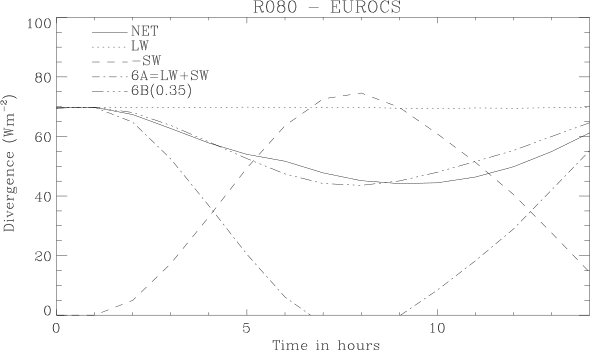
\includegraphics[width=3.5in]{div_r080}
    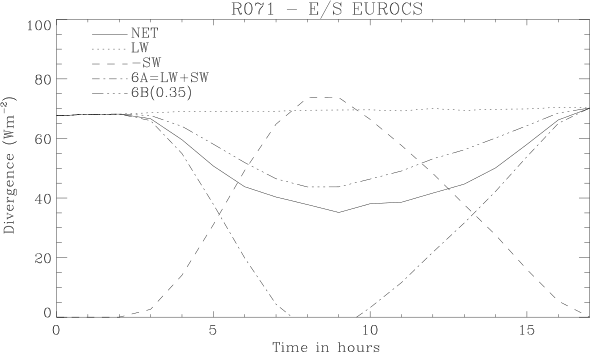
\includegraphics[width=3.5in]{div_r071}
  \end{centering}
  \captionarb{Time series from LES of $\Delta_\radf$ (solid),
    $\Delta_\radf^{LW} $ (dotted), $-\Delta_\radf^{SW} $ (dashed) and
    the 8A (dash-dot) and 9B (dash-dot-dot-dot) parametrizations of
    $\Delta_\radf$.}
  \label{fig:dradts}
\end{figure}

The 9C version attempted to remove the grid-dependence implied by the
summation over 3 grid-levels in (\ref{ctraddiv}) as follows:
\begin{enumerate}
\item the search for the level with maximum LW radiative
  cooling, $k_m$, is restricted to the top half of the mixed layer and 
  no higher than level NTML$+1$
\item to allow for the case where the radiative cooling is distributed
  roughly equally over two grid-levels, if the LW flux divergence in
  level $k_m-1$ is greater than half that in level $k_m$, then $k_m$
  is lowered one grid-level.
\item then, the cloud-top radiative flux change is initially
  calculated for LW and SW fluxes separately as:
  \begin{equation}
    \Delta_\radf = \radf_{k_m+1} - \radf_{k_{rb}}
    \label{ctraddiv_9c}
  \end{equation}
  where the base grid-level for the calculation, $k_{rb}$, is taken to
  be the higher of the base of the LW radiatively cooled layer and
  $z_h/2$, since cooling can only generate turbulence if it occurs in
  the upper part of the mixed layer.  For decoupled stratocumulus
  layers, $k_{rb}$ is further restricted to be above the top of the
  surface mixed layer.
\item finally, the flux divergence across grid-level $k_m+1$ is
  separated into cloudy and free-atmospheric contributions by
  extrapolating the free-atmospheric flux-gradient downwards.  The
  cloudy contribution is then included in $\Delta \radf$:
  \begin{equation}
    \Delta \radf = \Delta \radf + \Delta_{k_m+\f{3}{2}} \radf 
    - \Delta_{k_m+\f{5}{2}} \f{\Delta_{k_m+\f{3}{2}} z}{k_m+\f{1}{2}} \radf
    \label{ctraddiv_9c_inv}
  \end{equation}
\item As at 9B above, the calculations in (\ref{ctraddiv_9c}) and
  (\ref{ctraddiv_9c_inv}) are performed separately for LW and SW
  radiation before the two are combined using the empirical
  relationship in (\ref{eq:deltaf_emp})
\end{enumerate}

Further single column model tests with fine vertical resolution have shown 
the above calculations can still fail to accurately measure the radiative 
flux jump across the top of the cloud.  The methodology now recommended is 
to identify where the LW radiative cooling profile transitions from 
free-tropospheric rates above the cloud to stronger rates within it.  It 
entails only relatively minor changes to the first two steps of the 
algorithm above which become:
\begin{enumerate}
\item the search for the level with maximum LW radiative cooling, $k_m$, is 
restricted to the top half of the mixed layer and below $1.2 \, \zhe$ (rather 
than level NTML$+1$ used above)
\item if the LW flux divergence in level $k_m+1$ is relatively weak (less than 
double that in level $k_m+2$), we assume that level $k_m+1$ is actually typical 
of the free-troposphere and that $k_m$ must therefore be the inversion 
grid-level (despite having the strongest LW cooling).  Hence we lower 
$k_m$ by one so that it now marks the top of the mixed layer --- note that 
LW cooling within the inversion grid-level will be included in step 4 above 
(which is unchanged)
\end{enumerate}
These small changes were found sufficient to give a robust measure of 
$\Delta \radf$ for grids varying down to 20m spacing where the radiative 
flux profile is well resolved.

%------------------------------------------------------------------------
% APPENDIX: BUOYANCY PARAMETERS
%------------------------------------------------------------------------
\newpage
\section{Appendix: Derivation and definitions of the buoyancy parameters}
\label{app:buoyp}

Buoyancy is measured by the virtual temperature
\begin{equation}
  T_v = T(1 + c_v q_v - \ql - q_f) = T V_{fac}
  \label{Tv}
\end{equation}
where $c_v=(1/\epsilon) -1$ and $\epsilon$ is the ratio of the
molecular weights of water vapour and dry air (\mbox{i.e.}, $\epsilon
= M_v/M_a \approx 0.62198$).  The buoyancy flux is then given by
\begin{equation*}
  \wb  = \frac{g}{T_v}\, \overline{w'T_v'}
\end{equation*}
Linearising gives
\begin{equation*}
  \wb = g \left( \beta_T \overline{w'T_L'} + \beta_q \wqt + 
    \left( \beta_T \frac{L}{c_p} - \frac{1+c_v}{c_v} \beta_q \right)
    \overline{w'\ql'} \right) 
\end{equation*}
where the buoyancy parameters are given by

\begin{equation*}
  \beta_T  = \frac{1}{T}, \qquad \beta_q = \frac{c_v}{V_{fac}} 
\end{equation*}

In saturated cloudy air (see, for example, \cite{stage1981}), the
Clausius-Clapeyron equation can be used to calculate $
\overline{w'\ql'} $ (via $\ql' = q_t' - q_s' = q_t' - \alpha_L T'$) as
\begin{equation*}
  \overline{w'\ql'} = a_L( \wqt - \alpha_L \overline{w'T_L'} )
\end{equation*}
where 
\begin{equation*}
  \alpha_L  = \frac{\partial q_s}{\partial T} = \frac{\epsilon L q_s(T,p) }{R T^2}, \qquad
  a_L   = \frac{1}{1+L\alpha_L/c_p}
\end{equation*}
where R is the gas constant ($=287.05$).  Thus the buoyancy flux can
be written
\begin{equation*}
  \wb = 
\begin{cases}
  g \left( \beta_T \overline{w'T_L'} + \beta_q \wqt \right)
  & {\rm in\ unsaturated\ air} \\
  g \left( \tilde{\beta_T} \overline{w'T_L'} + \tilde{\beta_q} \wqt
  \right) & {\rm in\ saturated\ air}
\end{cases}
\end{equation*}
where 
\begin{eqnarray*}
  \tilde{\beta_T}  = \beta_T - \alpha_L \beta_c, &
  \tilde{\beta_q} & = \beta_q + \beta_c \\
  {\rm and}    &
  \beta_c & = a_L \left(   \frac{L}{c_p}     \beta_T 
    - \frac{1+c_v}{c_v} \beta_q \right) 
\end{eqnarray*}

Note that here $\tilde{\beta_T}$ and $\tilde{\beta_q}$ are strictly
{\em in}-cloud parameters, while their definitions in boundary layer
code prior to 8A were grid-box mean.  Thus, here, any necessary
$C_F$-weighting must be included explicitly, as in (\ref{eq:wb_cont}).

In all the above, if $T$ is less than the melting point of ice then
the latent heat of sublimation, $L_s = L + L_f$, is used in place of
$L$.

%------------------------------------------------------------------------
% APPENDIX: MIXING RATIOS
%------------------------------------------------------------------------
\newpage
\section{Appendix: changing between specific humidities and mixing ratios}
\label{app:mixratio}

Denote wet density by 
\begin{equation*}
  \rho = \rho_y + \rho_v + \rhol + \rho_{f}
\end{equation*}
where $\rho_y$ is the density of dry air and the other $\rho$ are
vapour, liquid and frozen water respectively.  Mixing ratios and
specific humidities are then defined as
\begin{equation*}
  m_v = \frac{\rho_v}{\rho_y}  q_v = \frac{\rho_v}{\rho} 
\end{equation*}

When specific quantities are mixed, the turbulent diffusion equations,
(\ref{cons_eqn_scal}) and (\ref{cons_eqn_uv}), have $\rho$ as the wet
density.  This is then consistent with the conservation of globally
integrated quantities such as moisture.  For example, neglecting
spherical geometry for simplicity:
\begin{equation}
  \int (\rho_v + \rhol + \rho_{f})\, d\underline{x} = 
  \int \rho (q_v + \ql + q_{f}) \,d\underline{x} = \int \rho q_t \, d\underline{x}
\label{moisture_cons}
\end{equation}

When mixing ratios are used, the momentum equations,
(\ref{cons_eqn_uv}), remain unchanged and the wet density still
appears.  This makes the reasonable assumption that all moisture
components should be included in the momentum budget.  For moisture
conservation, (\ref{moisture_cons}) can be rewritten in terms of
mixing ratios as
\begin{equation*}
  \int (\rho_v + \rhol + \rho_{f})\, d\underline{x} = 
  \int \rho_y (m_v + \ml + m_{f}) \,d\underline{x} = \int \rho_y m_t \, d\underline{x}
\end{equation*}
Thus $\rho$ in (\ref{cons_eqn_scal}) is replaced with $\rho_y$ for
$\chi = m_t$ and $\thetal$ when mixing ratios are passed into the
boundary layer code.  

For surface exchange, JULES initially approximates the surface air density as 
$\rho_* = p_S/(R T_S)$ (where the subscript $S$ denotes the surface values and $R$ 
the gas constant for dry air, 287 JK$^{-1}$kg$^{-1}$).  If a more accurate calculation 
of surface air density is requested, following Eqs (1) to (6) of 
\cite{Webbetal1980} we then calculate the wet or dry surface air densities (to be 
used when the atmospheric humidity is specific or mixing ratio, respectively) as:
\begin{eqnarray*}
     \rho_{0} & =& \rho_*/(1+(1/\epsilon-1)q_S) \\
     \rho_{y0} & =& \rho_*/(1+(1/\epsilon)m_{vS})
\end{eqnarray*}
where, in each case, the surface humidity is taken as the surface saturated humidity 
over open sea but over land and ice surfaces this is likely to be inappropriate 
and so the driving level humidity is used (typically the lowest model level).

Note that $\thetal$ itself is defined in terms
of mixing ratios as:
\begin{equation}
  \thetal = T - \frac{L_c}{c_{pd}} \ml 
  - \frac{L_c+L_f}{c_{pd}} m_f + \frac{g}{c_{pd}} z  
  \label{sl_defn}
\end{equation}

For saturation calculations a version of QSAT is used that is
switchable between input specific and mixing ratio variables.  The
rate of change of $q_s$ with temperature is also used in the boundary
layer code (see e.g. appendix~\ref{app:buoyp}):
\begin{equation*}
  \frac{ d q_{sat} }{ dT } = \frac{\epsilon L q_{sat} }{RT^2}
\end{equation*}
In fact this expression should really be converted to work for
specific quantities and so simply changing to mixing ratios will
improve the accuracy of this calculation.

Finally, in appendix~\ref{app:buoyp} virtual temperature is defined in
terms of specific variables as
\begin{equation*}
  T_v = T ( 1 + c_v q_v - q_l )
\end{equation*}
In terms of mixing ratios this becomes
\begin{equation*}
  T_v = \frac{T ( 1 + m_v/\epsilon )}{ 1 + m_v + m_l }
\end{equation*}
Linearising, however, gives
\begin{equation*}
  T_v = T ( 1 + c_v m_v - m_l )
\end{equation*}
Thus, the same level of approximation as is currently used is
maintained simply by changing specific variables to mixing ratios.

Additional points to note are:
\begin{enumerate}
\item the diagnostic of screen humidity, $q$1.5m, will remain as a
  specific humidity. Similarly RH1.5m will remain defined in terms of
  specific quantities, \mbox{i.e.}, $q$1.5m$/q_s$1.5m
\item all other moisture diagnostics (\mbox{e.g.}, latent heat fluxes
  and increments) will simply switch to being mixing ratios if mixing
  ratios are selected - no conversion will be made.
\item it is important to note that RHOKM will be wet density times
  $K_m$ while RHOKH will be dry density times $K_h$
\end{enumerate}

%------------------------------------------------------------------------
% APPENDIX: frictional heating
%------------------------------------------------------------------------
\section{Appendix: including the heating from turbulence dissipation}
\label{app:fricheat}

An estimate of the true molecular dissipation rate, $\epsilon_{mol}$,
can be obtained by assuming local equilibrium in the budget of subgrid
TKE (SKE). Then the sum of the inputs from resolved kinetic energy,
plus that from subgrid buoyancy effects, must equal the dissipation.
The SKE budget is
\begin{equation}
  d SKE/dt = S + T + B + \epsilon_{mol}
\label{ske_budg}
\end{equation}
where the shear production, S, is essentially the resolved KE
dissipation term.  Note that the buoyancy term B appears in
(\ref{ske_budg}) which indicates that some of the energy from resolved
scale dissipation (i.e. S) should be consumed in doing work against
buoyancy (at least in stable BLs) thus leaving less energy to be
finally dissipated as heat. Note though that CBLs will generate
additional dissipation (and hence heating) through the buoyancy term.
Note that from an atmospheric budget viewpoint the transport term, T,
can be neglected as it will integrate vertically to zero. Locally,
vertical variations could be important but it will be ignored because
finally the heating source is implemented through an integral over the
BL.

So, this estimate of the molecular dissipation rate should appear as
an additional heating source term, (following \cite{zhang1999}):
\begin{equation*}
  \frac{\partial \thetal}{\partial t} =
  \left[\frac{du}{dz}\tau_x + \frac{dv}{dz}\tau_y  + B \right] / (\rho c_p)
\end{equation*}
Tests in the SCM showed the heating rate gradients can be very large
near the surface.  Hence to avoid stability problems (since this
heating increment must be added after the implicit calculation of the
stress (and heat flux) profiles) the increments are summed over the
levels within the BL (i.e. up to \zh) and then that total heating is
applied as a linear decrease from the surface to zero over \zh.

%------------------------------------------------------------------------
% APPENDIX: OPERATIONAL FUDGES
%------------------------------------------------------------------------
\section{Appendix: Operational modifications}
\label{app:opmods}

The operational global forecast model has been found to give improved
performance on NWP Index parameters when the following modifications
to its local $Ri$-based scheme are used.  In (\ref{asymp_ml}), the
definition of $\lambda_m$ only is altered to
\begin{equation*}
  \lambda_m = \mbox{max}\left[40,\, 0.3 \zloce, 2 h_B \right]
\end{equation*}
and both $\lambda_m$ and $\lambda_h$ are not reduced (to 40m) above
the boundary layer top.  It is possible these modifications point to
problems with the definition of the boundary layer depth and the use
of a Prandtl number of unity with no stability dependence in the local
scheme.  Both these issues are under further investigation.

\newpage
%------------------------------------------------------------------------
% APPENDIX: UKCA INPUTS
%------------------------------------------------------------------------
\section{Appendix: Inputs to UKCA}

The UKCA chemistry and aerosols sub-model takes a number of boundary
layer diagnostics as input. For a list of these and a brief
explanation of how they are used see the table below.  If any changes
modify the results for these variables it will prevent UKCA jobs from
regressing. If the changes are significant it would be prudent to
discuss them with the UKCA code owner before lodging the change.

\begin{table}[htp]
  \begin{center}
    \begin{tabular}{|p{0.5cm}|p{0.7cm}|p{6cm}|p{6cm}|}
      \hline
      \multicolumn{4}{|c|}{Boundary layer inputs to UKCA} \\
      \hline
      Sec   &  Item   &  Description   & Use in UKCA \\
      \hline
      0 & 24   & SURFACE TEMPERATURE AFTER TIMESTEP  &  dry deposition \\
      0 & 25   & BOUNDARY LAYER DEPTH AFTER TIMESTEP &  dry deposition, bl nucleation and call to tr\_mix \\
      0 & 26   & ROUGHNESS LENGTH AFTER TIMESTEP  &  dry deposition \\
      0 & 233  & SURFACE TEMPERATURE ON TILES K  &  dry deposition \\
      0 & 234  & ROUGHNESS LENGTH ON TILES m  &  dry deposition \\ 
      3 & 60   & RHOKH\_MIX &  call to tr\_mix \\
      3 & 64   & DTRDZ\_CHARNEY\_GRID &  call to tr\_mix \\
      3 & 65   & GRID-LEVEL OF SML INVERSION (kent) &  call to tr\_mix \\
      3 & 66   & Rho * entrainment rate (we\_lim) &  call to tr\_mix \\
      3 & 67   & Fraction of the timestep (t\_frac) &  call to tr\_mix \\
      3 & 68   & zrzi &  call to tr\_mix \\
      3 & 69   & GRID-LEVEL OF DSC INVERSION (kent) &  call to tr\_mix \\
      3 & 70   & Rho * entrainment rate dsc &  call to tr\_mix \\
      3 & 71   & Fraction of the timestep dsc &  call to tr\_mix \\
      3 & 72   & zrzi dsc &  call to tr\_mix \\
      3 & 73   & ZHSC Top of decoupled layer &  call to tr\_mix \\
      3 & 217  & SURFACE HEAT FLUX W/M2 &  dry deposition \\
      3 & 230  & 10 METRE WIND SPEED ON C-GRID & calculate sea salt emissions \\
      3 & 401  & Dust Emissions div 1  & GLOMAP dust scheme \\
      3 & 402  & Dust Emissions div 2  & GLOMAP dust scheme \\
      3 & 403  & Dust Emissions div 3  & GLOMAP dust scheme \\
      3 & 404  & Dust Emissions div 4  & GLOMAP dust scheme \\
      3 & 405  & Dust Emissions div 5  & GLOMAP dust scheme \\
      3 & 406  & Dust Emissions div 6  & GLOMAP dust scheme \\
      3 & 430  & Dust Friction velocity (U*) on tiles &  dry deposition \\
      3 & 462  & STOMATAL CONDUCTANCE ON PFTS (M/S) &  dry deposition \\
      3 & 465  & FRICTION VELOCITY &  dry deposition  \\
      3 & 473  & TURBULENT KINETIC ENERGY &  ACTIVATE cloud scheme \\
      \hline
    \end{tabular}
  \end{center}
\end{table}

%------------------------------------------------------------------------
% APPENDIX: NOTATION
%------------------------------------------------------------------------
\section{Appendix: Notation}
\label{app:not}

\begin{flushleft}
  \begin{tabular}{|l|l|}
    \hline
    \multicolumn{2}{|c|}{Finite difference notation} \\
    \hline
    $z_k$ & height of the $\theta$-level $k$ \\
    $z_{k+\frac{1}{2}}$ & height of half-level above $\theta$-level $k$ \\
    $\Delta_k$ & indicates a finite difference between $\theta$-levels $k$ and
    $k-1$ \\ 
    $\Delta_{k+\frac{1}{2}}$ & indicates a finite difference between
    half-levels $k+\frac{1}{2}$ and $k-\frac{1}{2}$ \\
    $\Delta$ & note: real change (\mbox{i.e.}, not necessarily
    finite-difference) in a parameter \\ 
    & across the capping inversion (see (\ref{dbinv}) and following text) \\
    \hline
  \end{tabular}
\end{flushleft}

\begin{flushleft}
  \begin{tabular}{|l|l|}
    \hline
    \multicolumn{2}{|c|}{Model variables} \\
    \hline
    $\theta_l$, $\thetavl$  & thermodynamic variables defined by (\ref{thetal})
    and (\ref{thetavl}) \\
    $T_v$, $\theta_v$ & virtual temperature and potential temperature, \\ 
    & defined by (\ref{Tv}) and in section (\ref{sec:parxs}) \\
    $b$               & buoyancy ($=g T_v'/T_v$) \\
    $q_t$, $q_v$, $q_s$, $\ql$, $q_f$ & specific humidities: \\ 
    & total, vapour, saturated, liquid and frozen water, respectively \\ 
    $C_F$, $C_F^l$, $C_F^f$ & cloud fraction and the liquid and frozen water
    parts, respectively \\
    ${\cal H}$ &  total heat flux (net radiative plus turbulent, Kms$^{-1}$) \\
    \hline
  \end{tabular}
\end{flushleft}

\begin{flushleft}
  \begin{tabular}{|l|l|}
    \hline
    \multicolumn{2}{|c|}{Thresholds} \\
    \hline
    $C_t$ & ($=1.1$) threshold for ratio of layer $q_t$-gradients in cumulus
    diagnosis \\ 
    $\Gamma_{\rm inv}$ & ($=1.1$) threshold on ratio of environment to parcel 
    $\theta_v$ gradients \\
    & for identifying capping inversions above the LCL \\
    SC\_CFTOL & ($=0.1$) $C_F$ threshold for recognising the presence of Sc \\
    $\Delta_{k_{ct}} \thetavl / \Delta_{k_{ct}} z < 10^{-3}$ & threshold
    (in Km$^{-1}$) for initial diagnosis of {\em well-mixed} DSC layers \\
    $D_t$  & ($=0.1$) threshold for the ratio of buoyancy consumption to
    production \\ 
    & before decoupling occurs \\
    \hline
  \end{tabular}
\end{flushleft}

\begin{flushleft}
  \begin{tabular}{|l|l|}
    \hline
    \multicolumn{2}{|c|}{Layer definitions and parameters} \\
    \hline
    SML & surface-based mixed layer \\
    NTML & top $\theta$-level within SML \\
    NTPAR & top $\theta$-level reached by parcel ascent \\
    DSC & decoupled stratocumulus (mixed layer) \\
    NTDSC & top $\theta$-level within DSC layer \\
    NBDSC & bottom $\theta$-level within DSC layer \\
    NTLOC & top $\theta$-level below which $Ri<1$ \\
    \zh & height of top of SML (potentially subgrid) \\
    \zhsc & height of top of DSC layer (potentially subgrid) \\
    \zbase & height of base of DSC layer (subgrid) \\
    \zhpar & height of half-level at top of parcel ascent \\
    \zloc & height of half-level marking `top' of local $Ri$-based mixing \\ 
    & (where $Ri>1$) \\
    $z_i$ & generic inversion height \\
    $z_c$ & cloud depth \\
    $\zml$ & mixed layer depth \\
    $\kmsurf$, $\khsurf$ & $K$ profiles for surface-driven turbulence (in SML) \\
    $\kmtop$, $\khtop$ & $K$ profiles for cloud-top-driven turbulence \\ 
    & (calculated for both DSC and SML) \\
    LCL & lifting condensation level \\
    \hline
  \end{tabular}
\end{flushleft}

\begin{flushleft}
  \begin{tabular}{|l|l|}
    \hline
    \multicolumn{2}{|c|}{Other parameters} \\
    \hline
    $\gamma_{\thetal}$ & gradient adjustment term, given by (\ref{gradadj}) \\
    $w_m$ & scaling velocity for momentum mixing in the SML \\
    & (used in $\kmsurf$, $\gamma_{\thetal}$ 
    and the SML parcel perturbation, $\theta_v'$) \\
    $w_*$ & `standard' convective velocity scale for a cloud-free convective \\
    &  boundary layer, $ w_*^3 = \zhe \wbs $ \\
    $u_*$ & friction velocity (here includes the orographic component) \\
    $w_e$, $\tilde{w_e}$ & entrainment velocity and compensated to allow for 
    subsidence (ms$^{-1}$) \\
    $w_S$ & subsidence velocity (ms$^{-1}$) \\ 
    $\Delta_\radf $ & cloud-top net radiative divergence, calculation given in
    (\ref{ctraddiv}) \\
    $\alpha_t$ & parameter in entrainment parametrization, (\ref{we_parm}) \\
    $\tau_{rc}$, $z_{rc}$ & parameters in perturbation calculation,
    (\ref{dscd_pert}), \\ 
    & for initial identification of and $\zml$ calculation for DSC layers \\ 
    $a_L$, $\alpha_L$, $\beta_T$, $\beta_q$, $\tilde{\beta_T}$, $\tilde{\beta_q}$
    &  buoyancy parameters, defined in appendix~\ref{app:buoyp} \\
    \hline
  \end{tabular}
\end{flushleft}

\newpage

\bibliographystyle{plainnat}
\bibliography{refs}

\end{document}                     % Every document must end with this.






